\title{Adaptive Control of Unmanned Aerial Vehicles - Theory and Flight Tests}
\author{
        Suresh K. Kannan \\
        Controls Group, Systems Department\\
        United Technologies Research Center\\
        East Hartford, CT 06118\\
            \and
        Girish V. Chowdhary\\
        Department of Aeronautics and Astronautics\\
        Massachusetts Institute of Technology\\
        Cambridge, MA 02139
                \and
        Eric N. Johnson\\
        School of Aerospace Engineering\\
        Georgia Institute of Technology\\
        Atlanta, GA 30332
}
\date{\today}


\documentclass[12pt]{article}
\usepackage{hyperref}
\usepackage{amsmath,latexsym,amssymb,subeqnarray,bm,textcomp}
\usepackage{verbatim,alltt}
\usepackage{amsthm}
\usepackage{cancel,ifthen,wrapfig}
\usepackage{fullpage}
\usepackage{subfigure}
%\usepackage{todonotes}
\hypersetup{colorlinks=true,linkcolor=blue,citecolor=red,pdftitle=Adaptive Control of Unmanned Aerial Vehicles - Theory and Flight Tests,pdfauthor=Suresh K. Kannan}
%\usepackage{showkeys}
%\newenvironment{remark}{\begin{quotation}}{\end{quotation}}
\newtheorem{remark}{Remark}
\newtheorem{assumption}{Assumption}
%\newenvironment{note}{\begin{quotation}}{\end{quotation}}
\newtheorem{note}{Remark}
\newtheorem{lemma}{Lemma}
%\newenvironment{theorem}{\begin{quotation}}{\end{quotation}}
\newtheorem{theorem}{Theorem}
\newtheorem{corollary}{Corollary}
\newtheorem{definition}{Definition}
\newtheorem{fact}{Fact}
\newtheorem{claim}{Claim}
%\newcommand{\mreal}[1][]{\ensuremath{\mathbb{R}^{#1}}}
%Editing shortcuts
%\newcommand{\todo}[1]{\label{todo:#1}\textbf{(comt:{#2})}}
\newcommand{\comt}[1]{\textbf{(comt:{#1})}}
% Standard referencing shortcuts
\newcommand{\eq}[1]{Eqn~(\ref{#1})}
\newcommand{\eqrng}[2]{Eqns.~(\ref{#1}-\ref{#2})}
\newcommand{\sys}[1]{(\ref{#1})}
\newcommand{\sysrange}[2]{(\ref{#1} - \ref{#2})}
\newcommand{\lem}[1]{Lemma~\ref{#1}}
\newcommand{\thm}[1]{Theorem~\ref{#1}}
\newcommand{\ass}[1]{Assumption~\ref{#1}}
\newcommand{\asspg}[1]{Assumption~\ref{#1} (pg. \pageref{#1})}
\newcommand{\cor}[1]{Corollary~\ref{#1}}
\newcommand{\fig}[1]{\mbox{Fig.~\ref{#1}}}
\newcommand{\rem}[1]{Remark~\ref{#1}}
\newcommand{\secti}[1]{Section~\ref{#1}}
\newcommand{\chap}[1]{Chapter~\ref{#1}}
\newcommand{\appdx}[1]{Appendix~\ref{#1}}
\newcommand{\defn}[1]{Definition~\ref{#1}}
\newcommand{\defnpg}[1]{Definition~\ref{#1} (pg. \pageref{#1})}
\newcommand{\fct}[1]{Fact~\ref{#1}}
\newcommand{\clm}[1]{Claim~\ref{#1}}
\newcommand{\pg}[1]{Page~\pageref{#1}}
% Standard math shortcuts
\newcommand{\inv}[1]{\ensuremath{#1^{-1}}}
\newcommand{\dom}[1]{\ensuremath{\mathcal{D}_{#1}}}
\newcommand{\real}[1]{\ensuremath{\mathcal{R}^{#1}}}
\newcommand{\lvl}{\ensuremath{\Omega}}
\newcommand{\nulldom}[1]{\ensuremath{\mathcal{C}_{#1}}}
\newcommand{\mreal}[1]{\ensuremath{\mathcal{R}^{#1}}}
\newcommand{\tr}[1]{\ensuremath{tr\left(#1\right)}}
\newcommand{\defined}{\triangleq}
\newcommand{\ssys}[1]{\ensuremath{(#1)}}



%%%%%%%%%%%%%%%%%%%%%%%%%%%%%%%%%%%%%%%%%%%%%%%%%%%%%%%%


\newcommand{\fhat}{\ensuremath{\hat{f}}}
\newcommand{\ghat}{\ensuremath{\hat{\bfg}}}
\newcommand{\xd}{\ensuremath{\dot{x}}}
\newcommand{\xdd}{\ensuremath{\ddot{x}}}
\newcommand{\xbar}{\ensuremath{\bar{\bfx}}}

\newcommand{\delh}{\ensuremath{\hat{\delta}}}
\newcommand{\deldes}{\ensuremath{\delta_{des}}}
\newcommand{\Del}{\ensuremath{\Delta}}
\newcommand{\Delbar}{\ensuremath{\bar{\Del}}}
\newcommand{\Deld}{\ensuremath{\Del'}}
\newcommand{\nuad}{\ensuremath{\nu_{ad}}}
\newcommand{\nuhad}{\ensuremath{\bar{\nu}_{ad}}}
\newcommand{\nur}{\ensuremath{\nu_r}}
\newcommand{\nuh}{\ensuremath{\nu_h}}
\newcommand{\nucr}{\ensuremath{\nu_{cr}}}
\newcommand{\nubcr}{\ensuremath{\bar{\nu}_{cr}}}
\newcommand{\nulc}{\ensuremath{\nu_{lc}}}
\newcommand{\domd}{\ensuremath{\mathcal{D}}}
\newcommand{\sigbar}{\ensuremath{\bar{\sigma}}}

\newcommand{\il}{inner loop}
\newcommand{\ol}{outer loop}

% Short cuts for q,omega,p,v derivatives, commands and desired
\newcommand{\bfa}{\ensuremath{a}}
\newcommand{\bfe}{\ensuremath{e}}
\newcommand{\bfer}{\ensuremath{e_r}}
\newcommand{\bfg}{\ensuremath{g}}
\newcommand{\bfp}{\ensuremath{p}}
\newcommand{\bfq}{\ensuremath{q}}
\newcommand{\bfr}{\ensuremath{r}}
\newcommand{\bfv}{\ensuremath{v}}
\newcommand{\bfx}{\ensuremath{x}}
\newcommand{\bfz}{\ensuremath{z}}
\newcommand{\bfw}{\ensuremath{w}}
\newcommand{\bfalpha}{\ensuremath{\alpha}}
\newcommand{\bfdelta}{\ensuremath{\delta}}
\newcommand{\bfepsilon}{\ensuremath{\epsilon}}
\newcommand{\bfzeta}{\ensuremath{\zeta}}
\newcommand{\bftheta}{\ensuremath{\theta}}
\newcommand{\bfomega}{\ensuremath{\omega}}
\newcommand{\bfsigma}{\ensuremath{\sigma}}
\newcommand{\qd}{\ensuremath{\dot{\bfq}}}
\newcommand{\od}{\ensuremath{\dot{\bfomega}}}
\newcommand{\pd}{\ensuremath{\dot{\bfp}}}
\newcommand{\vd}{\ensuremath{\dot{\bfv}}}

\newcommand{\qc}{\ensuremath{\bfq_c}}
\newcommand{\oc}{\ensuremath{\bfomega_c}}
\newcommand{\pc}{\ensuremath{\bfp_c}}
\newcommand{\vc}{\ensuremath{\bfv_c}}
\newcommand{\ac}{\ensuremath{\bfa_c}}
\newcommand{\alc}{\ensuremath{\bfalpha_c}}


\newcommand{\qdes}{\ensuremath{\bfq_{des}}}
\newcommand{\odes}{\ensuremath{\omega_{des}}}
\newcommand{\pdes}{\ensuremath{p}_{des}}
\newcommand{\vdes}{\ensuremath{v}_{des}}

% x
\newcommand{\xc}{\ensuremath{x_c}}
\newcommand{\xr}{\ensuremath{x_r}}

%Ref model shortcuts
\newcommand{\qrm}{\ensuremath{\bfq_{r}}}
\newcommand{\orm}{\ensuremath{\bfomega_{r}}}
\newcommand{\prm}{\ensuremath{\bfp}_{r}}
\newcommand{\vrm}{\ensuremath{\bfv}_{r}}
\newcommand{\alrm}{\ensuremath{\alpha}_{r}}
\newcommand{\arm}{\ensuremath{a}_{r}}


%Pseudo, control shortcuts
\newcommand{\aldes}{\ensuremath{\bfalpha_{des}}}
\newcommand{\ades}{\ensuremath{\bfa_{des}}}
\newcommand{\adesdelf}{\ensuremath{\bfa_{des_{\delf}}}}
\newcommand{\adesq}{\ensuremath{\bfa_{des_{\bfq}}}}
\newcommand{\alcrm}{\ensuremath{\bfalpha_{cr}}}
\newcommand{\acrm}{\ensuremath{\bfa_{cr}}}
\newcommand{\alpd}{\ensuremath{\bfalpha_{pd}}}
\newcommand{\apd}{\ensuremath{\bfa_{pd}}}
\newcommand{\alad}{\ensuremath{\bfalpha_{ad}}}
\newcommand{\aad}{\ensuremath{\bfa_{ad}}}
\newcommand{\alhad}{\ensuremath{\bar{\bfalpha}_{ad}}}
\newcommand{\ahad}{\ensuremath{\bar{\bfa}_{ad}}}
\newcommand{\alh}{\ensuremath{\bfalpha_{h}}}
\newcommand{\ah}{\ensuremath{\bfa_{h}}}



%Estimated pseudocontrol
\newcommand{\alhat}{\ensuremath{\hat{\bfalpha}}}
\newcommand{\ahat}{\ensuremath{\hat{\bfa}}}


% Actuator shortcuts
\newcommand{\delm}{\ensuremath{\bfdelta_m}}
\newcommand{\delf}{\ensuremath{\bfdelta_f}}
\newcommand{\delfq}{\ensuremath{\begin{bmatrix}\delta_f}\\ q\end{bmatrix}}
\newcommand{\delmd}{\ensuremath{\dot{\bfdelta}_m}}
\newcommand{\delfd}{\ensuremath{\dot{\bfdelta}_f}}
\newcommand{\delhm}{\ensuremath{\hat{\bfdelta}_m}}
\newcommand{\delhf}{\ensuremath{\hat{\bfdelta}_f}}
\newcommand{\delmdes}{\ensuremath{\bfdelta_{m_{des}}}}
\newcommand{\delfdes}{\ensuremath{\bfdelta_{f_{des}}}}
\newcommand{\delhd}{\ensuremath{\dot{\hat{\bfdelta}}}}
\newcommand{\delhmd}{\ensuremath{\dot{\hat{\bfdelta}}_m}}
\newcommand{\delhfd}{\ensuremath{\dot{\hat{\bfdelta}}_f}}
\newcommand{\delmin}{\ensuremath{\bfdelta_{min}}}
\newcommand{\delmax}{\ensuremath{\bfdelta_{max}}}
\newcommand{\deldmin}{\ensuremath{\dot{\bfdelta}_{min}}}
\newcommand{\deldmax}{\ensuremath{\dot{\bfdelta}_{max}}}

\newcommand{\delbar}{\ensuremath{\bar{\delta}}}
\newcommand{\delubar}{\ensuremath{\underbar{\delta}}}
\newcommand{\deldbar}{\ensuremath{\bar{\dot{\delta}}}}

% proof shortcuts
\newcommand{\ozhot}{\ensuremath{\mathcal{O}^2(\tilde{\bfz})}}
\newcommand{\nztil}{\ensuremath{\|\tilde{Z}\|}}
\newcommand{\nVt}{\ensuremath{\|\tilde{V}^T\|_F}}
\newcommand{\nWt}{\ensuremath{\|\tilde{W}^T\|_F}}
\newcommand{\nZtsq}{\ensuremath{\|\tilde{Z}\|_F^2}}
\newcommand{\nZt}{\ensuremath{\|\tilde{Z}\|_F}}
\newcommand{\nZ}{\ensuremath{\|Z\|_F}}
\newcommand{\WsT}{\ensuremath{W^{*T}}}
\newcommand{\WtT}{\ensuremath{\tilde{W}^T}}
\newcommand{\VtT}{\ensuremath{\tilde{V}^T}}
\newcommand{\Zbar}{\ensuremath{\bar{Z}}}
\newcommand{\zt}{\ensuremath{\tilde{\bfz}}}
\newcommand{\Zt}{\ensuremath{\tilde{Z}}}
\newcommand{\Vt}{\ensuremath{\tilde{V}}}
\newcommand{\Wt}{\ensuremath{\tilde{W}}}



% nested saturation section

\newcommand{\signslaw}{\ensuremath{\sigma_n(y_n+\sigma_{n-1}(y_{n-1}+\cdots+\sigma_1(y_1)))}}
\newcommand{\signslawshort}{\ensuremath{\sigma_n(y_n + \sigma_{n-1}(\cdots\sigma_1(y_1)))}}
\newcommand{\consatl}{conventional saturation}
\newcommand{\linsatl}{linear saturation}
\newcommand{\linsat}{linear saturation}
\newcommand{\Linsat}{Linear Saturation}
\newcommand{\consat}{conventional saturation}
\newcommand{\Consat}{Conventional Saturation}
\newcommand{\vecsat}{vector valued saturaion}
\newcommand{\Vecsat}{Vector Valued Saturaion}

% k-cascade systems
\newcommand{\nonenk}{\ensuremath{n_1+\hdots+n_k}}
\newcommand{\Nk}{\ensuremath{N_k}}
\newcommand{\sze}{\ensuremath{z}}
\newcommand{\sxi}{\ensuremath{\xi}}
\newcommand{\szedes}{\ensuremath{\sze}_{des}}
\newcommand{\sxides}{\ensuremath{\sxi}_{des}}
\newcommand{\delsze}{\ensuremath{\delta_\sze}}
\newcommand{\delsxi}{\ensuremath{\delta_\sxi}}
\newcommand{\delszedes}{\ensuremath{\delta_{\sze_{des}}}}
\newcommand{\delsxides}{\ensuremath{\delta_{\sxi_{des}}}}
\newcommand{\delszeh}{\ensuremath{\hat{\delta}_\sze}}
\newcommand{\delsxih}{\ensuremath{\hat{\delta}_\sxi}}
\newcommand{\nusze}{\ensuremath{\nu_\sze}}
\newcommand{\nusxi}{\ensuremath{\nu_\sxi}}
\newcommand{\fsze}{\ensuremath{\phi}}
\newcommand{\fsxi}{\ensuremath{\gamma}}
\newcommand{\fszedes}{\ensuremath{\fsze_{des}}}
\newcommand{\fsxides}{\ensuremath{\fsxi_{des}}}
\newcommand{\fszedesdelsze}{\ensuremath{\fsze_{des_{\delsze}}}}
\newcommand{\fszedessxi}{\ensuremath{\fsze_{des_{\sxi}}}}
\newcommand{\fhsze}{\ensuremath{\hat{\fsze}}}
\newcommand{\fhsxi}{\ensuremath{\hat{\fsxi}}}

\newcommand{\ellip}{\ensuremath{\mathcal{E}}}


% some shortcuts for denoting approximate functions
\newcommand{\var}[2]{%
\ifthenelse{\equal{#2}{}}%
{\ensuremath{\breve{#1}^{#2}}}%
{\ensuremath{\breve{#1}^{(#2)}}}%
}
\newcommand{\vardes}[2]{\ensuremath{#1|#2}}

%\newcommand{\varndes}[2]{\ensuremath{#1~#2}}

\ifx\pdfoutput\undefined
  \usepackage[dvips,final]{graphicx}  % using latex+dvips
  \usepackage[dvips,usenames]{color}
\else
  \usepackage[pdftex,final]{graphicx} % using pdflatex
  \usepackage[pdftex,usenames]{color}
\fi
\graphicspath{{./figures/}}
\usepackage[disable]{todonotes}


\begin{document}
\maketitle
\listoftodos
\begin{abstract}
Typically, unmanned aerial vehicles are underactuated systems i.e., they have fewer independent control inputs than degrees of freedom. In a helicopter for example, the body-axis roll, pitch, yaw and altitude axis are fully actuated. However, lateral and longitudinal translational motion is only possible by tilting the thrust vector. This chapter develops a 6 degree-of-freedom flight control algorithm that can track both position and attitude trajectories. Approximate inverse models for vehicle attitude and position dynamics are used for feedback linearization leading to an inner-loop that tracks attitude and angular rate and an outer-loop that tracks position and velocity commands. A single adaptive element is used to compensate for inversion errors (uncertainty) in both loops. A key challenge in realizing an adaptive control design on real aircraft is dealing with actuator magnitude and rate saturation. Such saturation elements cannot be easily captured in inverse models and leads to incorrect learning in the adaptive element during periods of saturation. A mechanism to exactly remove such incorrect learning is provided. Additionally, nonlinear reference models are introduced to mitigate the risks of the closed loop system entering regions of the flight envelope that result in loss-of-controllability. The resulting adaptive controller accepts trajectory commands comprising of desired position, velocity, attitude and angular velocity and produces normalized actuator signals required for flight control. A modification to the baseline adaptive control system is also provided that enables long-term retention of the uncertainty approximation within the adaptive element. This architecture is validated through flight-tests on several fixed wing and rotorcraft UAVs, including a $145~lb$ helicopter UAV (Yamaha R-Max or GTMax), a scale model fixed-wing aircraft (GTEdge), and a small ducted-fan (GTSpy).
\end{abstract}
%One method of dealing with such systems is to design controllers for two cascaded fully-actuated subsystems: an inner-loop attitude control system and an outer-loop velocity and position control system.
%The primary development and discussion will be one for a helicopter UAV, however the adaptive control architecture has been applied and successfully flown on fixed-wing aircraft as well.


\section{Introduction}
The US Department of Defense Integrated Unmanned Systems Roadmap \cite{dod:uavroadmap:2011} defines four levels of autonomy for Unmanned Systems. Level 1 involves manual operator control. Level 2 assumes automatic control while using humans to delegate waypoints. Level 3 assumes the UAV is capable of performing high-level activities using sensed data when given some directions by a human. Level 4 assumes that the UAV is capable of taking a top-level goal, breaking it into tasks and executing them along with the contingency replanning necessary to accomplish a top-level goal. Level 4 approaches the abstract and high-level goals that are provided to human soldiers in today's battlefield.

Level 2 behavior is available in almost all UAV's today. However, this accomplishment is after at least two decades of development with multiple efforts for each type of vehicle. The current U.S Department of Defense focus is on research, development and procurement of technologies that encompass Level 3 and Level 4 autonomous operations while assuming Level 2 is available. The key to developing fully autonomous Level 4 type behaviors is the ability to plan and also deal with contingencies. At the flight control system level this translates to the closed loop system being robust and adaptive to changes in the environment and vehicle dynamics. To motivate further, future Unmanned Systems will involve verification and validation using formal approaches where an amount of trust in autonomy is generated. Current conventional FAA certification practices will be superseded with certification methods that allow integration of UAV's into the civil airspace. One straightforward metric that may be used for 'trust in flight control' is the variance in trajectory tracking with uncertainty in the dynamics and environment. Consequently, the vehicles may be required to perform at their limits in order to maintain the required performance. Most current control systems still do not leverage the full flight envelope of small helicopters, at least, unless significant and expensive system identification and validation has been conducted.

Currently, fast algorithms to plan routes around obstacles are available\cite{Frazzoli.Dahleh.ea:JGCD02,Karaman.Frazzoli:IJRR11}. To be truly useful, these routes would include high-speed dashes, tight turns around buildings, avoiding dynamic obstacles and other required aggressive maneuvers. Allowing control saturation and adaptation allows higher level planning algorithms to provide optimistic trajectories which are then tracked by the flight controller to the best of the vehicles ability. The following is a description of some key elements that affect flight control stability and performance.

\emph{Parametric Uncertainty} arises from uncertainty in the mass, inertia properties, and aerodynamic characteristics. This limits the safe operational envelope of the vehicle to flight regimes where control designs are valid and parametric uncertainty is small. The effects of parametric uncertainty and unmodeled dynamics can be handled using a combination of system identification \cite{gavrilets:gnc:01,civita:ahs:02,mettler} and robust control techniques \cite{civita:gnc:02,gavrilets:gnc:02,civita:acc:03}.  However, system identification is expensive and when changes happen in real-time, for e.g., an unexpected payload is attached or deployed, the available previously-identified models may not fit the current aircraft configuration.  In this chapter, parametric uncertainty arises due to approximate inversion and appears as an unknown nonlinear function of the states and controls (unstructured). An adaptive element (neural network) is then used as a nonlinear function approximator to instantaneously cancel the inversion error.

\emph{Unmodeled Dynamics} arise when the vehicle model used for control design neglects parts of the real system's dynamics. Examples include the Bell-Hillier stabilizer bar and the flapping dynamics of the helicopter rotor blades. For most autonomous flight control work, the flapping dynamics may be safely neglected, whereas the Bell-Hillier stabilizer bar found on small rotorcraft cannot be ignored when high-bandwidth attitude control is desired. This chapter assumes state-feedback of rigid-body states keeping the control design simpler by leveraging the control design's robustness to unmodeled dynamics. Related adaptive designs that use an output-feedback controller formulation to explicitly deal with unmodeled dynamics are described in \cite{calise:automatica:2001} with experimental results in \cite{corban:gnc:2003}.

\emph{Actuator Magnitude and Rate Saturation} limit control authority and thus the closed loop stability and performance. Addressing input dynamics constitutes an important class of control design methods for systems with bounded actuation and include Sontag's universal formula approach using control Lyapunov functions \cite{lin:scl:91} and others \cite{bemporad:itac:97,pappas:cdc:95}. Avoiding saturation, however, usually results in either conservative or highly complex control laws leading to possibly very conservative domains of attraction and slow convergence. See \cite{bernstein:ijrnc:95} and the references therein for a survey of early work on constrained control. 


Other related works on rotorcraft control may be found in \cite{kendoul:itr:2006,kendoul:jgcd:2007,kendoul:jfr:2010} and a recent survey on guidance, navigation and control methods for rotorcraft is available in \cite{kendoul:jfr:2012}.


%A key aspect in the effective use of unmanned aerial vehicles(UAVs) for military and civil applications is their ability to accommodate changing dynamics and payload configurations automatically without having to rely on substantial system identification efforts. Variants of the Neural-Network (NN) based direct adaptive control methods have been used as enabling technologies for practical flight control systems that allow online adaptation to uncertainty. This technology has been successfully applied to the recent U.S. Air Force Reconfigurable Control for Tailless Fighter Aircraft (RESTORE) culminating in a successful flight demonstration \cite{calise:jgcd:01,brinker:jgcd:01} of the adaptive controller on the X-36. A combined inner-outer loop architecture was also applied for guidance and control of the X-33 \cite{johnson:jgcd:03} and evaluated successfully in simulation for various failure cases.

%Much adaptive control work on helicopters has concentrated on improving the tracking performance of attitude commands \cite{nakwan:jgcd:02,leitner:jgcd:97,rysdyk:jgcd:98}.

\begin{figure}
  \centering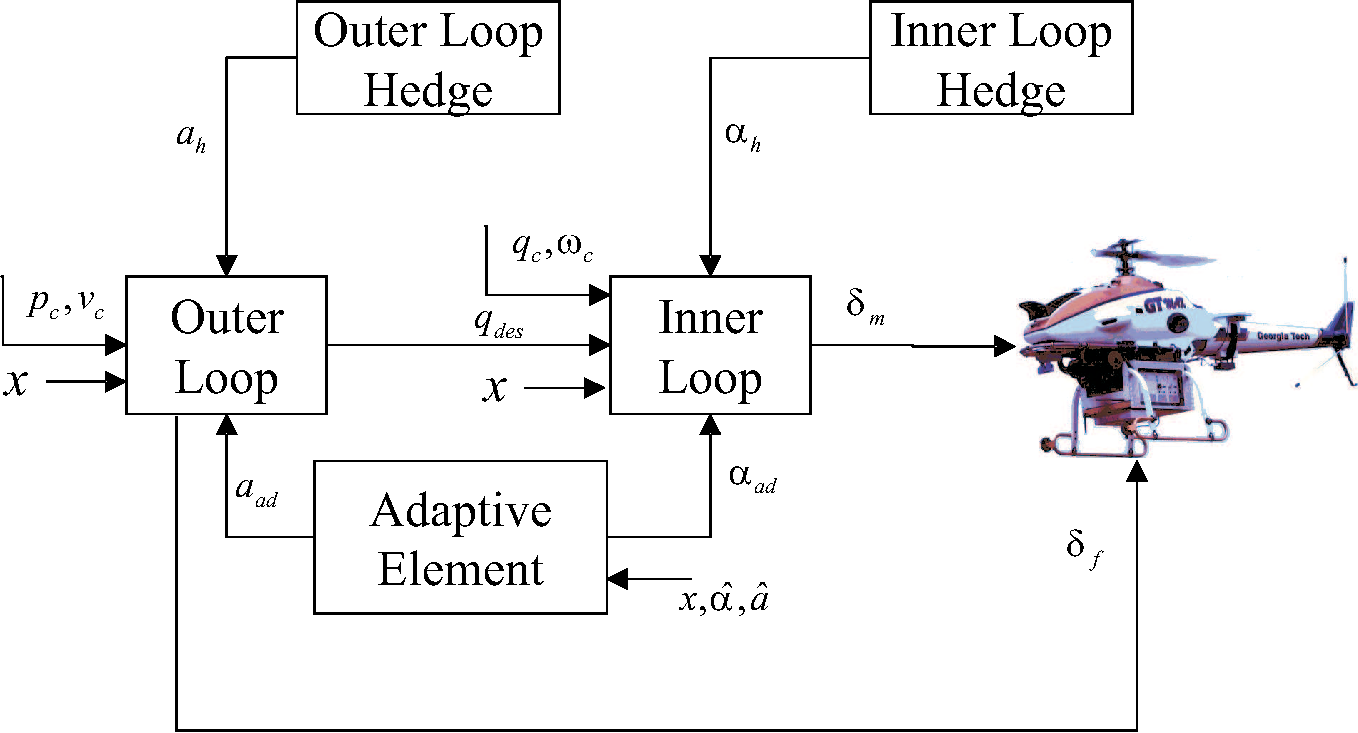
\includegraphics[width=0.7\columnwidth]{overallarch}
  \caption{Overall Architecture}
  \label{f:overallarch}
\end{figure}

\subsubsection*{Approach}
Helicopters have 6 degrees of freedom when considering just the rigid body modes and 4 independent controls are available to control them. Traditionally, the control variables lateral stick, $\delta_{lat}$, longitudinal stick, $\delta_{lon}$ and pedal, $\delta_{ped}$, control moments around the roll, pitch and yaw axes respectively. Finally, the collective input, $\delta_{coll}$ produces thrust along the main rotor shaft. The rotational dynamics are fully actuated whereas the translational dynamics are underactuated, but controllable. The rotor thrust has to be oriented using the aircraft's pitch and roll attitude to produce translational accelerations.

An overall architecture of the approach is shown in \fig{f:overallarch} with details in \fig{f:detailarch}. The outer loop is responsible for tracking desired translational accelerations. It generates $\delta_{coll}$ to vary rotor thrust along the main shaft and also generates the desired roll and pitch angles to orient the thrust vector to generate linear accelerations in these two underactuated degrees of freedom. Note here that the desired pitch and roll angles are commands to the inner-loop controller. In this respect the inner-loop acts like a (virtual) actuator as far as the outer-loop is concerned. Similarly, the inner-loop generates the actuator deflections necessary to control the rotational dynamics. Of course, here the inner-loop's output actuation signal is subject to the real actuator dynamics of the physical aircraft. In both loops, approximate models of the rotational (inner-loop) and translational (outer-loop) dynamics are dynamically inverted to produce the actuator deflections (and desired pitch and roll) necessary to achieve the desired angular and linear accelerations. These desired accelerations are generated using reference models dictating the desired ideal closed loop response. The cascaded inner-outer loop architecture used here is commonly employed in aerospace control applications due to the different dynamical time-scales of the two loops. {\color{red} Chapter ``Linear Flight Control Techniques for Unmanned Aerial Vehicles'' in this book discusses relevant details of cascaded control systems for UAVs.}

Adaptation is introduced in all six degrees of freedom to account for inversion errors arising from the approximate models used for inversion purposes. There is no particular restriction on the inversion that results in \emph{desired} actuator deflections to be bounded. Hence, at large desired accelerations, large actuator deflections may be commanded. Such saturation and dynamics will now appear in the adaptation training signal. This is also true in the case of the outer-loop because the commanded pitch and roll attitudes are now subject to the closed-loop dynamics of the inner-loop in addition to the actuator dynamics of the $\delta_{coll}$ actuator.

These nonlinearities appear in the stability analysis by way of their appearance in the error dynamics.  The, Pseudocontrol Hedging signal (PCH) is introduced in the outer-loop and inner-loop reference models in a manner that exactly removes elements of actuator saturation from the training signal for the adaptive element. The reference models themselves are nonlinear and prescribe the aggressiveness with which external commands are achieved. Thus, a comprehensive nonlinear, adaptive, trajectory tracking controller capable of adapting to uncertainties in all six degrees of freedom is developed. It must be noted that although the concrete example used throughout this chapter is one of a helicopter, the controller is not specific to a helicopter UAS. The development is generic, the only difference between a helicopter, a fixed-wing or other esoteric aircraft is the manner in which the available controls are categorized and the approximate models used for dynamic inversion purposes.

An underlying assumption of this work is that the nonlinear modeling error uncertainty can be approximated by a continuous function over the flight domain of an aircraft. The goal is to capture an approximation of the uncertainty using universal approximators such as neural networks. This universal approximation property guarantees that given a sufficient number neurons, there exists and an optimal set of (a priori unknown) weights that can approximate the uncertainty to a desired minimum approximation error. Once these weights are found, the learned dynamics can be used for online planning and health-monitoring purposes. The baseline adaptive laws developed in later sections of this chapter are designed to cancel instantaneous model error but do not necessarily guarantee convergence to the ideal weights during normal course of operation~\cite{ejohnson:jgcd:2005,kannan:cdc:2010,kannan:phd}. To alleviate this restriction, a modification, the \emph{concurrent learning adaptive control method} is introduced that greatly improves the convergence of weights to their ideal values in real-world conditions~\cite{Chowdhary:JGCD:10}. The method can in fact guarantee exponential convergence of the neural network weights to a neighborhood of their ideal values for linearly parameterized neural networks~\cite{Chowdhary:phd:2010}.

The adaptive controller described in this chapter has been extensively validated in flight on several aircraft regularly since 2002. The range of aircraft types include the Yamaha RMAX (GTMax) helicopter (\fig{f:helipic}), a 11-inch ducted-fan, the GTSpy (\fig{f:gtspypic}), a tail-less fixed-wing aircraft, the D6, and a high thrust-to-weight ratio aircraft, the GTEdge (\fig{f:gtedgepic}). The GTEdge is a tilt-body fixed-wing aircraft and capable of hovering on its propeller and flying like a regular fixed-wing aircraft. An interesting set of maneuvers performed by the GTEdge is the {hover$\Rightarrow$forward-flight$\Rightarrow$hover}, all using the same adaptive control system. The methods discussed here have also been implemented on smaller aircraft such as the GT Twinstar (Figure~\ref{f:twinstarpic}) a foam built twin-engine aircraft, the GT Logo a small rotorcraft of about 1 meter rotor diameter, and the GTQ \cite{chowdhary:gnc11:2011}, a miniature quadrotor. On the GT Twinstar, a variant of the algorithms presented here was used for flight with 25\% right wing missing~\cite{chowdhary:gnc:10:invited,chowdhary:infotech11:2011,Chowdhary:JGCD:12}.
\todo[inline,color=green]{Expand this list of Aircraft}
\todo[inline,color=green]{Need to refer to concurrent learning here}



\begin{figure}
  \centering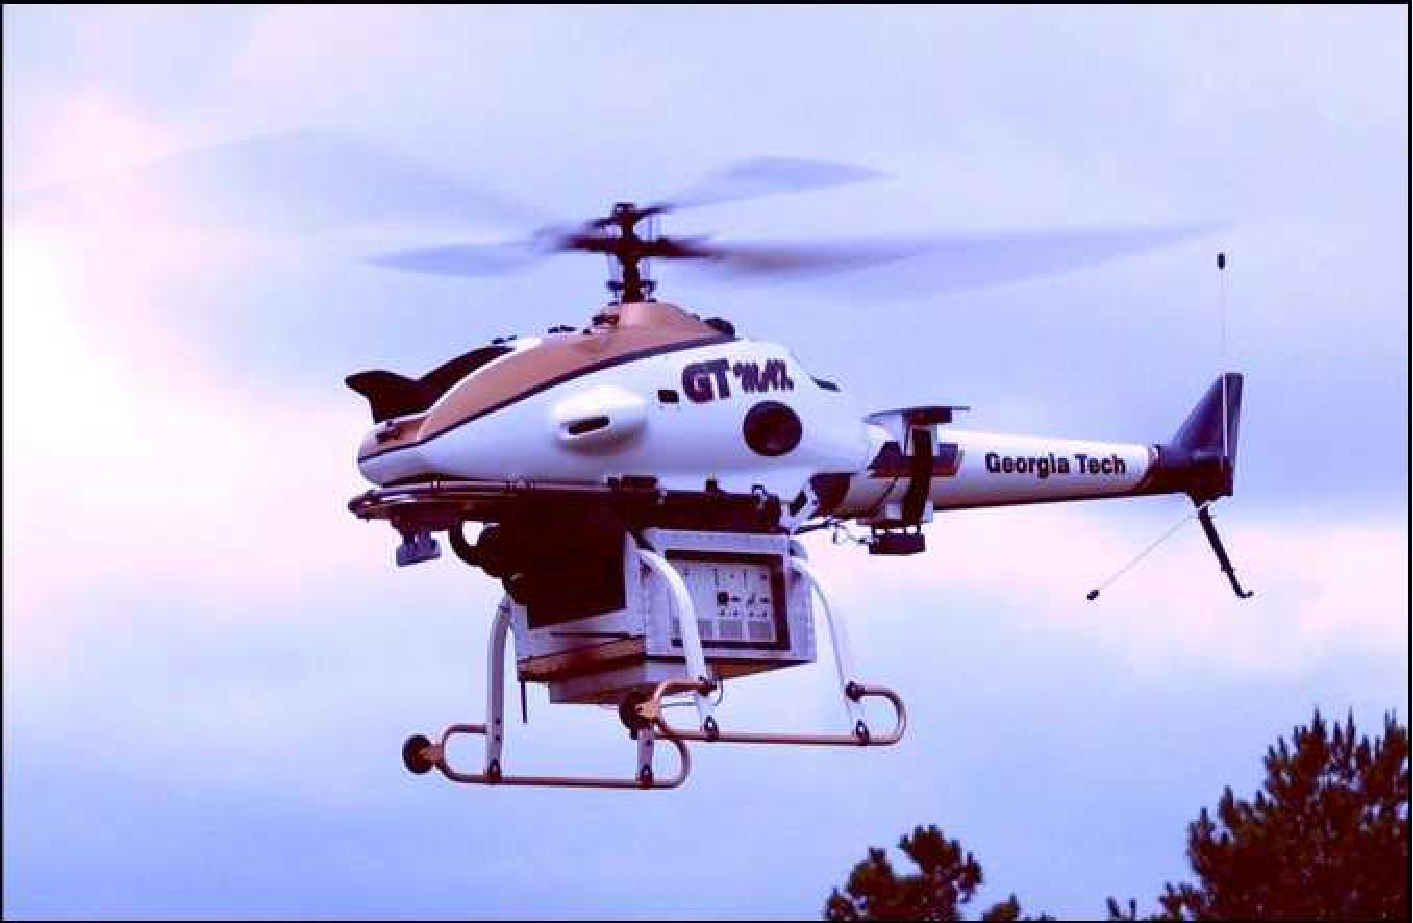
\includegraphics[width=0.7\columnwidth]{helipic}
  \caption{The GTMax Helicopter}
  \label{f:helipic}
\end{figure}
\begin{figure}
  \centering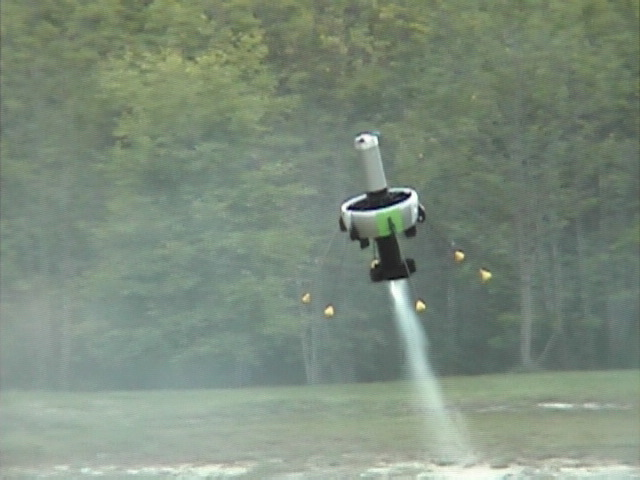
\includegraphics[width=0.7\columnwidth]{gtspy}
  \caption{The GTSpy 11-inch ducted fan}
  \label{f:gtspypic}
\end{figure}

\begin{figure}
  \centering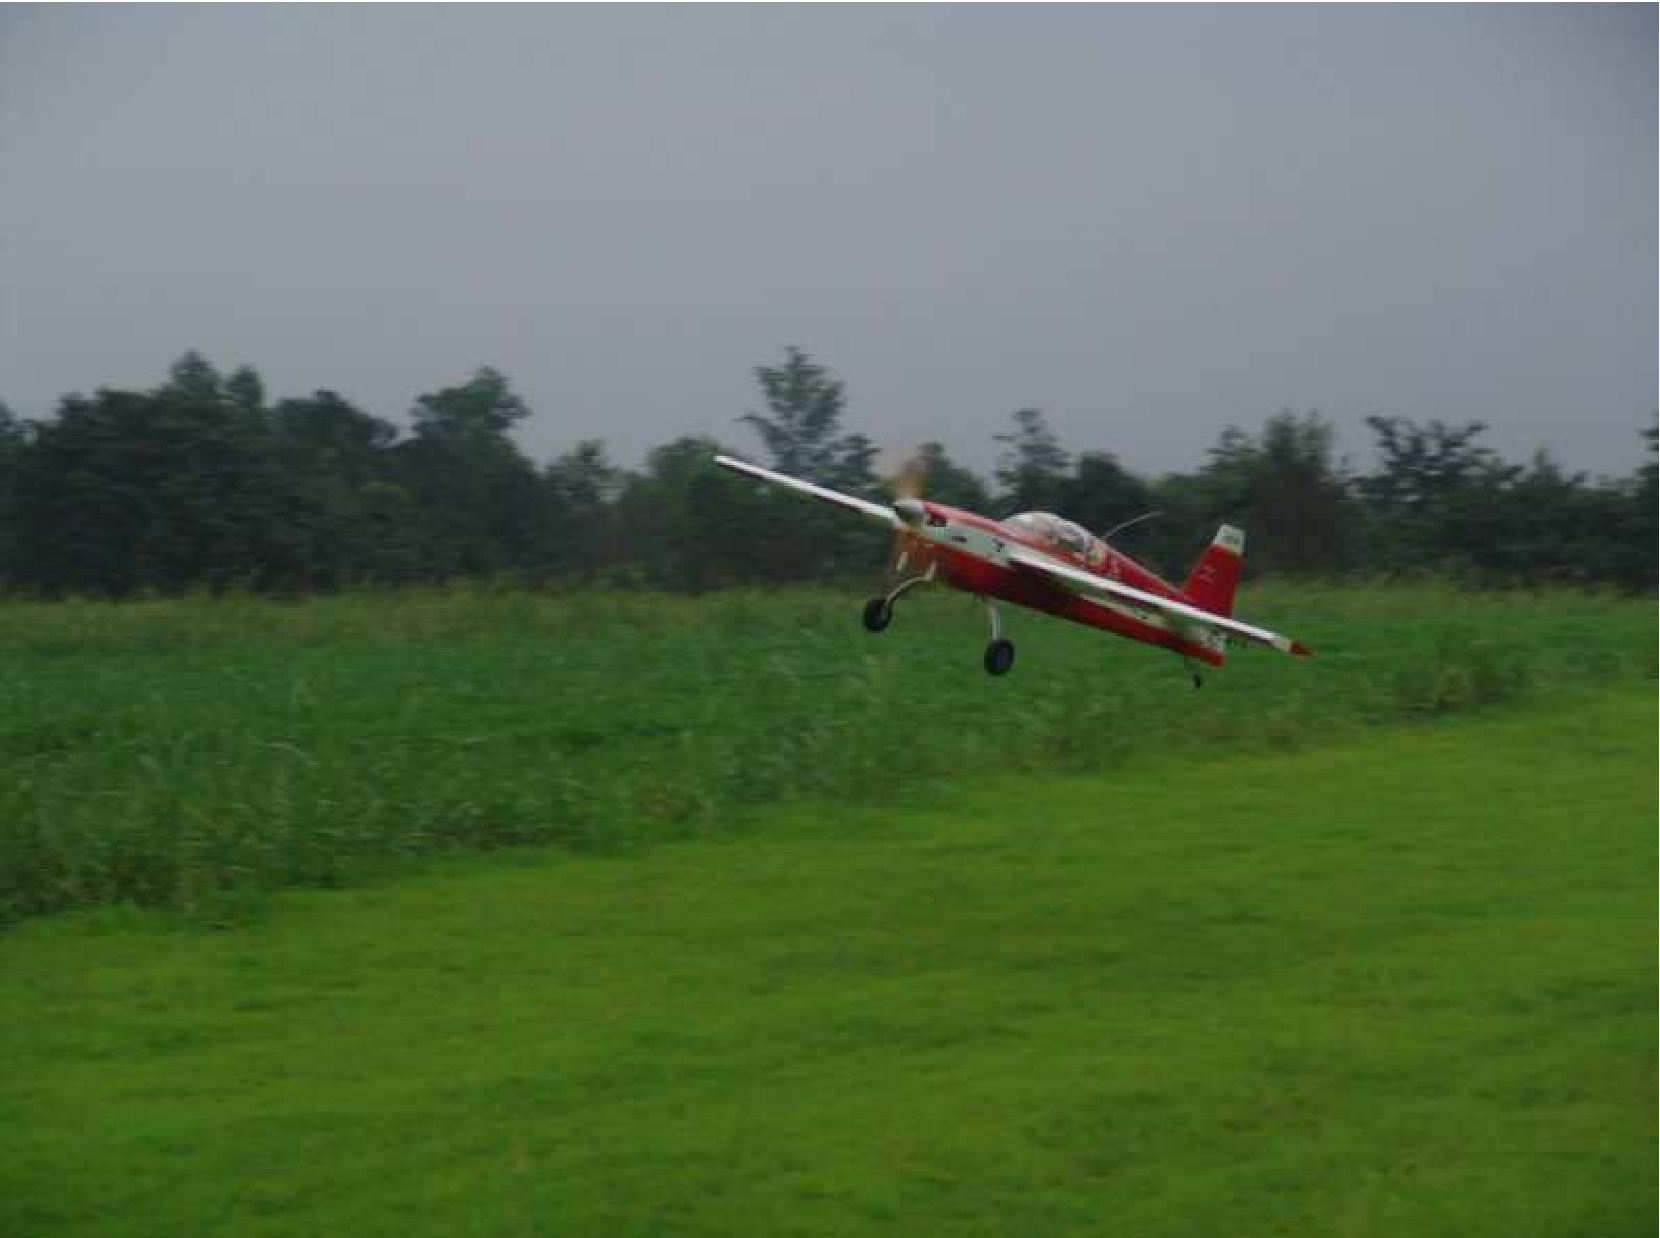
\includegraphics[width=0.7\columnwidth]{gtedge}
  \caption{The GTEdge aircraft with a high (greater than 1) thrust-to-weight ratio}
  \label{f:gtedgepic}
\end{figure}

\begin{figure}
  \centering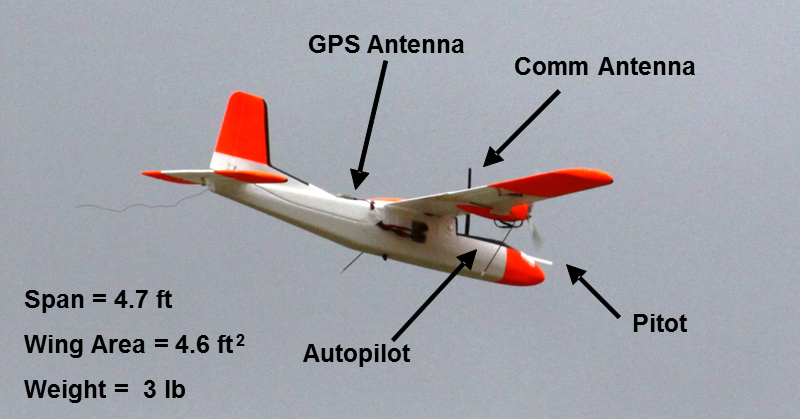
\includegraphics[width=0.7\columnwidth]{twinstar}
  \caption{The GTTwinstar foam built twin engine aircraft equipped for fault-tolerant control work (see e.g. \cite{chowdhary:infotech11:2011})}
  \label{f:twinstarpic}
\end{figure}


\section{Control of an Air Vehicle}
\subsection{Vehicle Dynamics}
Consider an air vehicle modeled as a nonlinear system of the form
%
\begin{eqnarray}
\pd &=& \bfv                                     \label{e:pdot}    \\
\vd &=& \bfa(\bfp,\bfv,\bfq,\bfomega,\delf, \delm)          \label{e:vdot}    \\
\qd &=& \qd(\bfq,\bfomega)                         \label{e:quatdot} \\
\od &=& \bfalpha(\bfp,\bfv,\bfq,\bfomega,\delf, \delm),
\label{e:omdot}
\end{eqnarray}
%
where, $\bfp \in \real{3}$ is the position vector, $\bfv \in
\real{3}$ is the velocity of the vehicle, $\bfq \in \real{4}$ is the
attitude quaternion and $\bfomega \in \real{3}$ is the angular
velocity. \eq{e:vdot} represents translational dynamics and
\eq{e:omdot} represents the attitude dynamics. Together, they represent rigid body dynamics and flat-earth kinematics as given in \cite{etkin72} and \cite{stevens:book:2003} and {\color{red} discussed in detail in the Chapter titled ``Linear Flight Control Techniques for
Unmanned Aerial Vehicles'' in this book}. \eq{e:quatdot}
represents the quaternion propagation equations \cite{stevens:book:2003}.
The use of quaternions, though not a minimal representation of
attitude, avoids numerical and singularity problems that
Euler-angles-based representations have. This enables the control
system to be all attitude capable as required for aggressive
maneuvering. The state vector $\bfx$ may now be defined as $ \bfx
\triangleq
\begin{bmatrix} \bfp^T & \bfv^T &\bfq^T &\bfomega^T\end{bmatrix}^T
$.

\begin{note}
The objective is to design a control system that can track a given position, velocity, attitude and angular rate trajectory. The consolidated trajectory command is given by
$\begin{bmatrix} \pc^T & \vc^T &\qc^T &\oc^T\end{bmatrix}^T$.
\end{note}

The control vectors are denoted by $\delf$ and $\delm$ and represent
actual physical actuators on the aircraft, where $\delf$ denotes the
primary force generating actuators and $\delm$ denotes the primary
moment generating actuators. For a helicopter, the main force
effector is the rotor thrust which is controlled by changing main
rotor collective $\delta_{coll}$. Hence $\delf \in \real{} =
\delta_{coll}$. There are three primary moment control surfaces, the
lateral cyclic $\delta_{lat}$, longitudinal cyclic $\delta_{lon}$,
and tail rotor pitch, also called the pedal input $\delta_{ped}$.
Hence, $\delm \in \real{3} =
\begin{bmatrix}
\delta_{lat} & \delta_{lon} & \delta_{ped}
\end{bmatrix}^T$.
In this chapter, the primary moment producing controls are treated as the inner-loop control effector whereas the $\delf = \delta_{coll}$, is treated as an outer-loop control effector. In general, both control inputs, $\delf$ and $\delm$, may
each produce both forces and moments. The helicopter is an under-actuated
system, and hence, the aircraft attitude, $\bfq$, is treated like a
\emph{virtual actuator} used to tilt the main rotor thrust in order to
produce desired translational accelerations in the longitudinal and lateral directions. Thus, it is not possible to track the commanded pitch, roll for a helicopter independently. It is only possible to track the heading component of the attitude $\qc$ and body-yaw rate $\bfomega_3$ independently. Direct control over the translational accelerations in the $body-z-axis$ is possible using $\delta_{coll}$.

The consolidated control vector $\bfdelta$ is defined as
\[
\bfdelta \triangleq
\begin{bmatrix}\delf^T &\delm^T\end{bmatrix}^T,
\]
the actuators themselves may have dynamics represented by
\begin{equation}
\label{e:g} \dot{\bfdelta} =
\begin{bmatrix}
\delmd \\
\delfd
\end{bmatrix}
=
\begin{bmatrix}
\bfg_m(\bfx,\delm,\delmdes)\\
\bfg_f(\bfx,\delf,\delfdes)
\end{bmatrix}
= \bfg(\bfx,\bfdelta,\deldes),
\end{equation} where $\bfg(\cdot)$ is generally unknown.
\begin{note}
It is possible to extend the architecture in order to treat actuator dynamics as simply another system in cascade with the translational and attitude dynamics and the control design would include an outer, inner and actuator loop with the actuator loop being the lowest block in the cascade. However unless the physical actuators need to be stabilized, their internal dynamics may be assumed to be asymptotically stable. In this chapter, rate and higher order dynamics are ignored, but magnitude-saturation will be handled explicitly. In can be shown that such an assumption is possible because the control design is robust to the unmodeled dynamics\cite{kannan:phd}.
\end{note}



\subsection{Control Design}\label{s:controller}
The control architecture is based on a  model reference adaptive control architecture (see \fig{f:detailarch}).%model for the inner and outer loops
\begin{figure}
%  \centering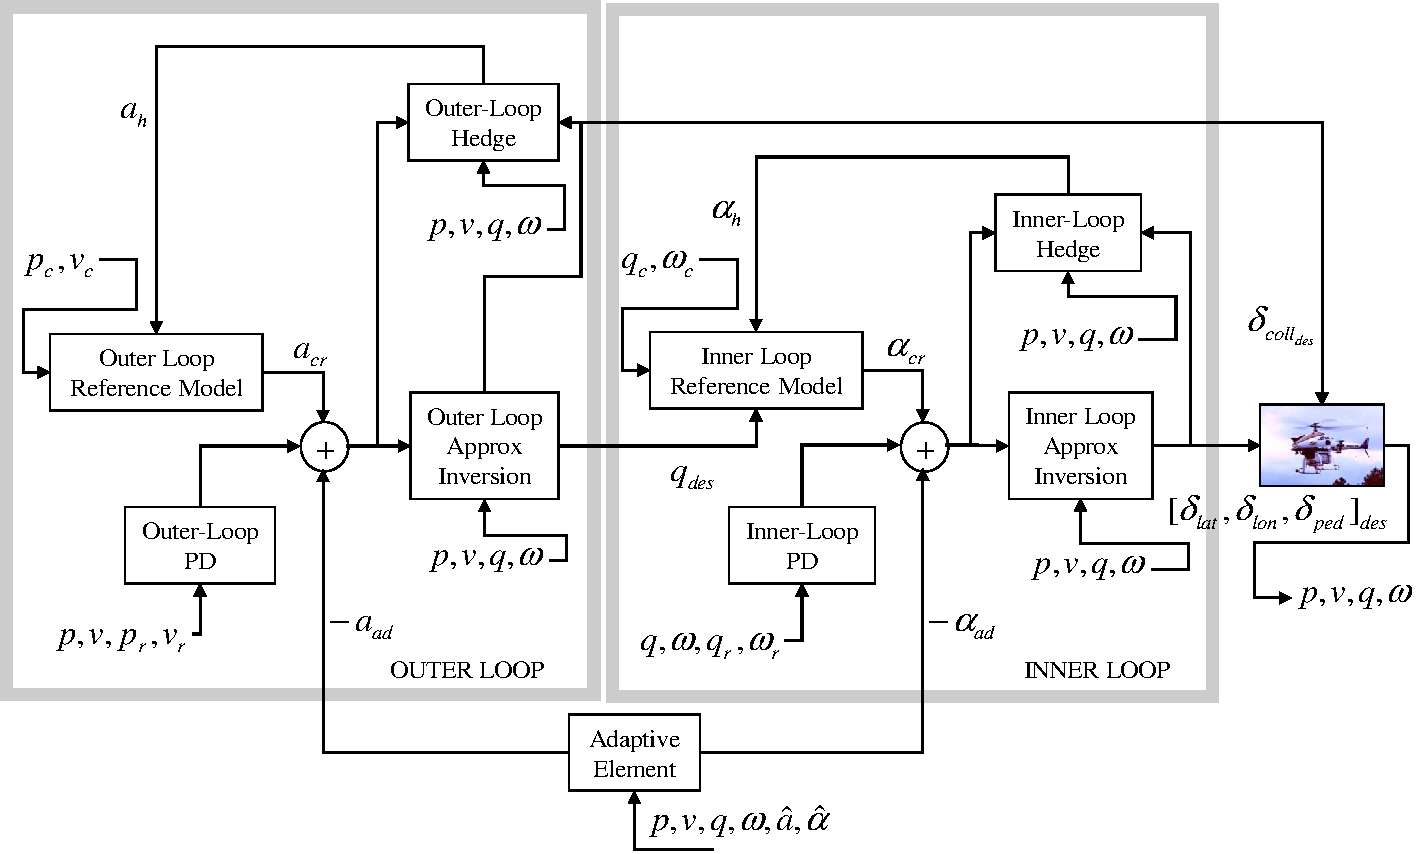
\includegraphics[]{detailarch}
  \centering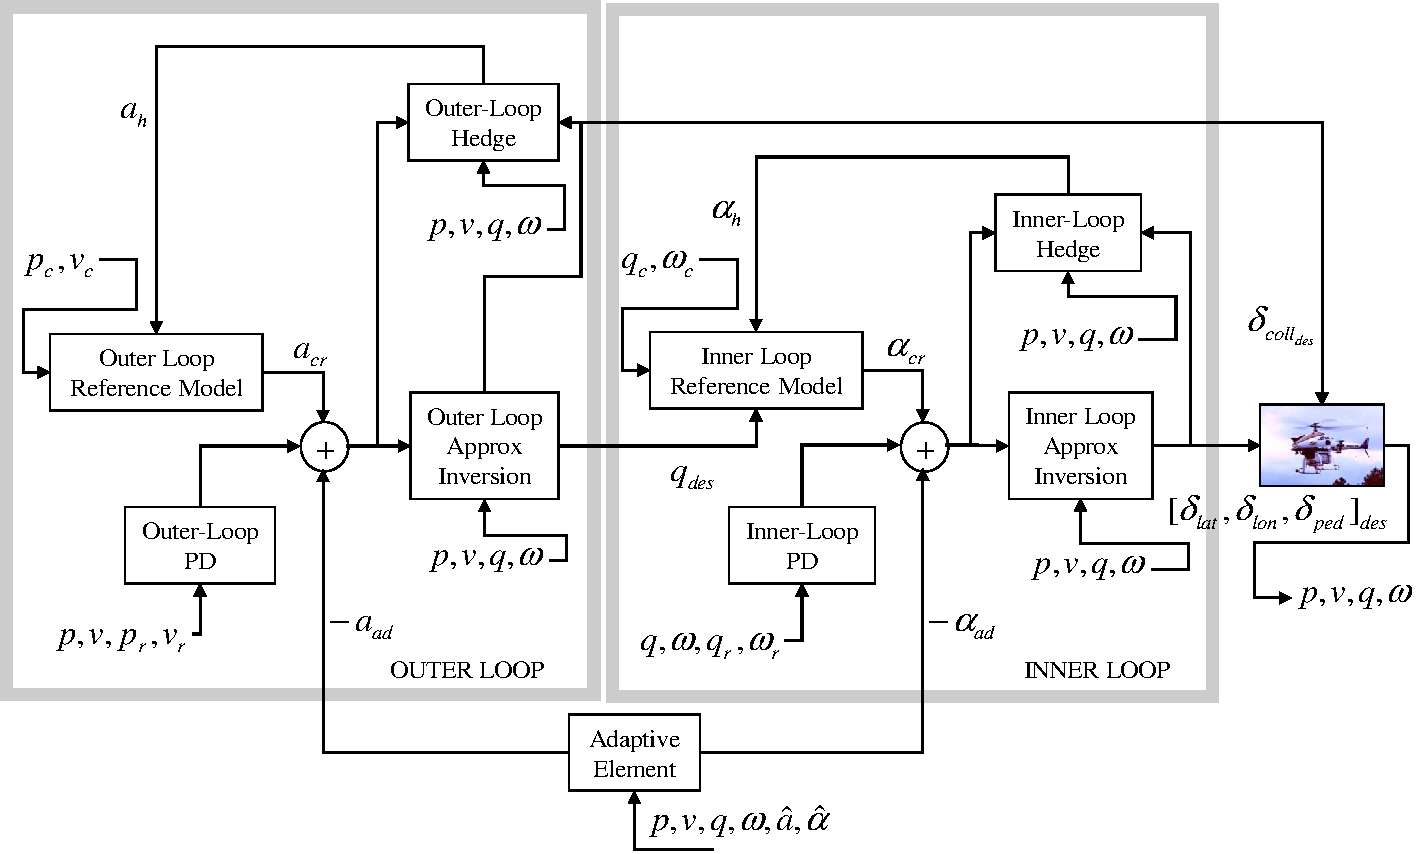
\includegraphics[width=1.4\textwidth,angle=90]{detailarch}
  \caption{Detailed inner and outer loop controller architecture for an autonomous helicopter.}
  \label{f:detailarch}
\end{figure}
Noting that \eq{e:pdot} and \eq{e:quatdot} represent exactly known kinematics, approximate models for translational acceleration, $\ahat$ and a model for angular acceleration, $\alhat$ need to be established.

\[
\begin{bmatrix}
\ades \\
\aldes
\end{bmatrix}
=
\begin{bmatrix}
\ahat (\bfp,\bfv,\qdes,\bfomega,\delfdes,\delhm)\\
\alhat(\bfp,\bfv,\bfq,\bfomega,\delhf,\delmdes)
\end{bmatrix},
\]
Here, $\ades$ and $\aldes$ are commonly referred to as the pseudocontrol
and represent desired accelerations. Additionally, $\delfdes,\delmdes,\qdes$ are the
control inputs and attitude expected to achieve the
desired pseudo-control. This form assumes that translational
dynamics are coupled strongly with attitude dynamics, as is the case
for a helicopter. From the outer-loop's point of view, $\bfq$
(attitude), is like a \emph{virtual actuator} that generates translational
accelerations and $\qdes$ is the desired attitude that the
outer-loop inversion expects will contribute towards achieving the
desired translational acceleration, $\ades$. The dynamics of $\bfq$
appears like actuator dynamics to the outer loop.

\begin{note}
Although the models are approximate, their functional dependence on vehicle rigid body and actuator states are stated accurately for completeness. It is likely that a specific approximate model that is introduced might drop some of this dependency.
\end{note}

\begin{note}
The attitude
quaternion $\qdes$ will be used to augment the externally commanded
attitude $\qc$ to achieve the desired translational accelerations.  Ideally, the trajectory generator would generate a commanded attitude $\qc$ that is consistent with the translational acceleration profile needed to track $\xc(t)$ and $\vc(t)$. If not, the outer-loop inverse takes care of correcting it by an amount necessary to achieve the desired translational accelerations in the longitudinal and lateral directions.
\end{note}

The models have a functional dependence on current actuator position. Because actuator positions are often not measured on small unmanned aerial vehicles, estimates of the actuator positions $\delhm, \delhf$
can be used. When the actuator positions are directly
measured, they may be regarded as known $\delhm = \delm$ and $\delhf
= \delf$. In fact, in the outer loop's case, good estimates of the roll and pitch attitude virtual actuators are
available using inertial sensors and a navigation filter.
%
The approximate models may now be inverted to obtain the desired control and attitude
%
\begin{equation}
\begin{split}
\label{e:inverselaw}
\begin{bmatrix}
\delfdes \\
\qdes
\end{bmatrix}
&=
\begin{bmatrix}
\inv{\ahat_{\delf}}(\bfp,\bfv,\adesdelf,\bfomega,\delhm)\\
\inv{\ahat_{\bfq}}(\bfp,\bfv,\adesq,\bfomega,\delhm)
\end{bmatrix}  \\
\delmdes &= \inv{\alhat}(\bfp,\bfv,\bfq,\bfomega,\delhf,\aldes),
\end{split}
\end{equation}
with $\adesdelf+\adesq = \ades$, $\ahat_{\delf},\ahat_{\bfq}$
formulated to be consistent with \eq{e:inverselaw} and where
actuator estimates are given by actuator models
\begin{equation}\label{e:ghat} \dot{\delh} =
\begin{bmatrix}
\delhfd \\
\delhmd
\end{bmatrix}
=
\begin{bmatrix}
\hat{\bfg}_f(\bfx,\delhf,\delfdes)\\
\hat{\bfg}_m(\bfx,\delhm,\delmdes)
\end{bmatrix}
= \ghat(x,\delh,\deldes).
\end{equation}
%

%In later sections, it will be shown that $\alhat$, can just be an
%approximate linear model of vehicle attitude dynamics and $\ahat$ a
%set of simple equations relating translational accelerations to the
%attitude of the vehicle.
%
Introducing the inverse control law \eq{e:inverselaw} into
\eq{e:vdot} and \eq{e:omdot} results in the following closed-loop
translational and attitude dynamics
%
\begin{align}\label{e:integrator}
\vd &= \ades  + \Delbar_{a}(\bfx,\bfdelta,\delh) -\ah \nonumber \\
 \od &= \aldes + \Delbar_{\bfalpha}(\bfx,\bfdelta,\delh) - \alh,
\end{align}
%
%
where%
\begin{equation}\label{e:Delbar}
\Delbar(\bfx,\bfdelta,\delh) =
\begin{bmatrix}
\Delbar_{a}(\bfx,\bfdelta,\delh) \\
\Delbar_{\bfalpha}(\bfx,\bfdelta,\delh)
\end{bmatrix}
=
\begin{bmatrix}
\bfa(\bfx,\bfdelta) - \ahat(\bfx,\delh) \\
\bfalpha(\bfx,\bfdelta) - \alhat(\bfx,\delh)
\end{bmatrix},
\end{equation}
are static nonlinear functions (model error) that arise due to
imperfect model inversion and errors in the actuator model $\ghat$. The main discrepancy between $g(\cdot)$ and $\ghat(\cdot)$ is the lack of a magnitude saturation function in $\ghat$. This is required in order to maintain invertibility.
The signals, $\ah$ and $\alh$, represent the pseudocontrol that
\emph{cannot be achieved} due to actuator input characteristics such as
saturation. If the model inversion were perfect and no magnitude-saturation
were to occur, $\Delbar,\ah$ and $\alh$ would vanish leaving only
the pseudocontrols $\ades$ and $\aldes$.

Two tasks now remain, (1) Stabilize the feedback linearized dynamics and (2) Address the effects of model error.
The desired accelerations may be designed as
%
\begin{equation}
\begin{split}\label{e:nu}
\ades  &= \acrm  + \apd  - \ahad \\
\aldes &= \alcrm + \alpd - \alhad,
\end{split}
\end{equation}
%
where $\acrm$ and $\alcrm$ are outputs of reference models for the
translational and attitude dynamics respectively. $\apd$ and $\alpd$
are outputs of proportional-derivative (PD) compensators; and
finally, $\ahad$ and $\alhad$ are the outputs of an adaptive element designed to cancel model error $\Delbar$. The effects of
input dynamics, represented by $\ah,\alh$ will first be addressed in
the following section by designing the reference model dynamics such
that they do not appear in the tracking error dynamics. The
reference model, tracking error dynamics, and boundedness are
discussed in the following sections with details of the adaptive element left to \appdx{s:network}.
%
\subsection{Reference Model and Hedging}
Any dynamics and nonlinearities associated with the actuators $\delm,
\delf$ have not yet been considered in the design. If they become
saturated (position or rate), the reference models will continue to
demand tracking as though full authority were still available.
Furthermore, the inner loop appears like an actuator with dynamics to
the outer loop. Practical operational limits on the maximum attitude
of the aircraft may have also been imposed in the inner-loop
reference model. This implies that the outer-loop desired attitude
augmentation $\qdes$ may not actually be achievable, or at the very
least is subject to the inner-loop dynamics.

If the reference model is designed as
\begin{equation}
\begin{split}
\label{e:rmnopch}
\vd_{r} &= \acrm (\prm,\vrm,\pc,\vc) \\
\od_{r} &= \alcrm(\qrm,\orm,\qc\oplus\qdes,\oc),
\end{split}
\end{equation}
where $\prm$ and $\vrm$ are the outer-loop reference model states
and $\qrm$, $\orm$, are the inner-loop reference model states.
The external command signal is $\bfx_c =
\begin{bmatrix}\pc^T & \vc^T & \qc^T & \oc^T\end{bmatrix}^T$. The attitude rotation desired by the outer loop is now added to the
commands for the inner loop controller. Here, $\qc \oplus \qdes$
denotes quaternion multiplication\cite{stevens2003} and effectively concatenates the two rotations.

If tracking error dynamics is computed by subtracting \eq{e:nu} from \eq{e:rmnopch}, the un-achievable acceleration $\ah, \alh$ will appear in the tracking error dynamics. When an adaptive element such as a neural network or integrator is introduced, these effects of input dynamics propagate into the training signal and eventually result in the adaptive element attempting to correct for them leading to incorrect adaptation.

Tackling this issue involves redesigning the reference model by subtracting the deficit accelerations (pseudo-control hedging)
\begin{align}
\label{e:pddrm}
\vd_{r} &= \acrm (\prm,\vrm,\pc,\vc) - \ah \\
\label{e:qddrm} \od_{r} &= \alcrm(\qrm,\orm,\qc\oplus\qdes,\oc) -
\alh,
\end{align}
$\ah$ and $\alh$ are the differences between commanded pseudocontrol
and an estimate of the achieved pseudocontrol. It is an estimate because actual actuator positions may not be known. Additionally, the aircraft state vector $\bfp,\bfv,\bfq,\bfomega$ are estimated using a Kalman Filter~\cite{henrik:jacic:2006,chowdhary:gnc11:2011}. However, for purposes of control design, they are assumed to be known and thus the virtual actuators such as attitude may be assumed to be known in the PCH computation. This assumption may have to be revisited in the case where the control/observer pair is not assumed to be separable, perhaps in a tough localization problem where the control inputs directly affect the observability of the aircraft states.

The PCH signals are given by
%
\begin{align} \label{e:ah}
\ah   &= \ahat (\bfp,\bfv,\qdes,\bfomega,\delfdes,\delhm) - \ahat(\bfp,\bfv,\bfq,\bfomega,\delhf,\delhm) \nonumber \\
      &= \ades                                - \ahat(\bfp,\bfv,\bfq,\bfomega,\delhf,\delhm)\\
\label{e:alh}
\alh  &= \alhat(\bfp,\bfv,\bfq,\bfomega,\delhf,\delmdes) - \alhat(\bfp,\bfv,\bfq,\bfomega,\delhf,\delhm)\nonumber\\
      &= \aldes                   -
      \alhat(\bfp,\bfv,\bfq,\bfomega,\delhf,\delhm).
\end{align}
%
The hedge signals $\ah$, $\alh$, do not directly affect
the reference model output $\acrm$, $\alcrm$, but do so only
through subsequent changes in the reference model states.

The command tracking error may now be defined as $\bfer$
\begin{equation}
\label{e:er} \bfer \triangleq
\begin{bmatrix}
\pc - \prm \\
\vc - \vrm \\
\tilde{Q}(\qc,\qrm) \\
\oc - \orm
\end{bmatrix},
\end{equation}
with corresponding command tracking error dynamics given by
\begin{equation}
\label{e:edotr} \dot{\bfer} =
\begin{bmatrix}
\vc - \vrm \\
\ac - (\acrm - \ah) \\
\oc - \orm \\
\alc - (\alcrm - \alh)
\end{bmatrix},
\end{equation}
The particular form of the reference model dynamics chosen for the translational dynamics, $\acrm$, and attitude dynamics, $\alcrm$, has profound effects on the overall response and controllability of the system. This is fully expounded in Chapter 4 of \cite{kannan:phd} and in \cite{kannan:cdc:2010b}. Also see \cite{kannan:acc:2003} for a discussion on the effects of reference model poles when various elements saturate.

\begin{comment}
A summary of the options for reference models is given here. A definition is useful at this point.
\begin{definition}
\label{def:nullcontstate} A state $x_0$ is said to be null
controllable in time $T
> 0$ if there exists an admissible control $\delta(t)$ such that the state
trajectory $x(t)$ of the system satisfies $x(0) = x_0$ and $x(T) =
0$. The set of all states that are null controllable in time $T$,
denoted by $\mathcal{C}(T)$, is called the null controllable region
in time $T$. The set of all such $x_0$ for $T\in[0,\infty]$ is call the null controllable region.
\end{definition}

Determining the null controllable region of a system is not trivial.
For linear systems, simple estimates may be found using the Circle
and Popov criteria as described in \cite{khalil:book:1992,pittet:cdc:1997}.
Less conservative estimates may be found as the result of an LMI
optimization as described in \cite{hu:book:2001}. For nonlinear systems of
the form \sys{e:simple:fxu}, there is no known method \cite{sontag:siam:1988,sontag:cdc:1988} to explicitly characterize a null controllable region
$\nulldom{x}$ where there always exists an admissible control which
can bring an initial state $x(0)$ back to the origin in finite time.
\end{comment}

As a summary, three reference models were considered.
\begin{itemize}
\item A \emph{Linear Reference Model} will attempt to elicit a linear response in the plant when no such response is possible (peaking) as the plant is nonlinear, especially with the magnitude saturation of actuators.
\item The \emph{Nested Saturation-based Reference Model} is an alternative to the linear reference model containing saturations functions appearing in a nested form and is based on the work by Teel\cite{teel:scl:1997,teel:itac:1996}. This form allows one to restrict the evolution of states in a prescribable manner.
\item The \emph{Constrained Linear Reference Model} is a special case of the nested saturation-based reference model, that is locally linear near the origin.
\end{itemize}

For the quadratic candidate Lyapunov functions chosen in \cite{kannan:phd}, only the nested-saturation and constrained linear reference models have their Lyapunov derivative bounds on the PCH signals $\ah,\alh$. In this chapter the constrained reference model is used with equations given later in \secti{s:helirefmodel}.

\begin{comment}
\begin{equation}
\label{e:refmodelgains}
\begin{bmatrix}
\apd \\
\alpd
\end{bmatrix} =
\begin{bmatrix}
R_p & R_d & 0   &   0 \\
0   & 0   & K_p &   K_d
\end{bmatrix}\bfe,
\end{equation}
\end{comment}


%
\subsection{Tracking error dynamics}
\label{s:trackingerrordynamics} The tracking error
vector is defined as, $\bfe$, as
\begin{equation}
\label{e:e} \bfe \triangleq
\begin{bmatrix}
\prm - \bfp \\
\vrm - \bfv \\
\tilde{Q}(\qrm,\bfq) \\
\orm - \bfomega
\end{bmatrix},
\end{equation}
%
where, $\tilde{Q}:\real{4}\times\real{4} \mapsto \real{3}$, is a
function~\cite{ejohnson:phd} that, given two quaternions results
in an error angle vector with three components. An expression for
$\tilde{\bm{Q}}$ is given by
%
\begin{align}
\label{e:quaterr}
\tilde{Q}(\bfp,\bfq) &= 2sgn(q_1p_1 + q_2p_2 + q_3p_3 + q_4p_4) \times \nonumber \\
&\qquad
\begin{bmatrix}
-q_1p_2 + q_2p_1 + q_3p_4 - q_4p_3 \\
-q_1p_3 - q_2p_4 + q_3p_1 + q_4p_2 \\
-q_1p_4 + q_2p_3 - q_3p_2 + q_4p_1
\end{bmatrix}.
\end{align}
%
The output of the PD compensators may be written as
%
\begin{equation}
\label{e:pdgains}
\begin{bmatrix}
\apd \\
\alpd
\end{bmatrix} =
\begin{bmatrix}
R_p & R_d & 0   &   0 \\
0   & 0   & K_p &   K_d
\end{bmatrix}\bfe,
\end{equation}
%
where, $R_p,R_d \in \real{3\times3}$, $K_p,K_d \in \real{3\times3}$
are linear gain positive definite matrices whose choice is discussed
below. The tracking error dynamics may be found by directly
differentiating \eq{e:e}
%
\[
\dot{\bfe} =
\begin{bmatrix}
\vrm - \bfv \\
\vd_{r} - \vd \\
\orm - \bfomega \\
\od_{r} - \od
\end{bmatrix}.
\]
%
Considering $\dot{\bfe}_2$,
%
\[
\begin{split}
\dot{\bfe}_2 &= \vd_{r} - \vd \\
          &= \acrm - \ah - \bfa(\bfx,\bfdelta) \\
          &= \acrm -\ades + \ahat(\bfx,\delh) - \bfa(\bfx,\bfdelta) \\
          &= \acrm -\apd -\acrm + \ahad + \ahat(\bfx,\delh) - \bfa(\bfx,\bfdelta)\\
          &= -\apd - (\bfa(\bfx,\bfdelta) - \ahat(\bfx,\delh) - \ahad) \\
          &= -\apd - (\Delbar_a(\bfx,\bfdelta,\delh) - \ahad), \\
\end{split}
\]
%
$\dot{\bfe}_4$ may be found similarly. Then, the overall tracking
error dynamics may now be expressed as
%
\begin{equation}\label{e:edot}
\dot{\bfe} = A\bfe + B\left[ \nuhad -
\Delbar(\bfx,\bfdelta,\delh)\right],
\end{equation} where, $\Delbar$ is given by \eq{e:Delbar},
\begin{equation}
 \nuhad = \begin{bmatrix}\ahad \\ \alhad
\end{bmatrix},
\label{e:AB} A =
\begin{bmatrix}
0     &    I     &    0    &   0 \\
-R_p  &   -R_d   &    0    &   0 \\
0     &    0     &    0    &   I \\
0     &    0     &   -K_p  & -K_d
\end{bmatrix},
B =
\begin{bmatrix}
0   &   0 \\
I   &   0 \\
0   &   0 \\
0   &   I
\end{bmatrix}.
\end{equation}
%
and so the linear gain matrices must be chosen such that $A$ is
Hurwitz. Now, $\nuhad$ remains to be designed in order to cancel
the effect of $\Delbar$.


Note that commands, $\delmdes,\delfdes,\qdes$, do not appear in
the tracking error dynamics. PCH allows adaptation to continue when
the actual control signal has been replaced by any arbitrary signal
and thus allows switching between manual and automatic flight during
flight tests without any transients. Furthermore, if the actuator is considered ideal and the actual
position and the commanded position are equal, addition of the PCH
signal $\ah$, $\alh$ has no effect on any system signal.

%
The adaptive signal $\nuhad$ contains two terms
\[
\nuhad = \nuad + \nur = \begin{bmatrix} \aad + \bfa_r \\
\alad + \bfalpha_r\end{bmatrix},
\]
where $\nuad$ is the output of the Single Hidden Layer (SHL) Neural Network (NN) described in
\secti{s:network}. For an air vehicle with adaptation in all degrees
of freedom, $\nuad \in \real{6}$, where the first three outputs,
$\aad$, approximates $\Del_a$ and the last three outputs, $\alad$,
approximate $\Del_{\alpha}$ and is consistent with the definition of
the error in \eq{e:e}.  The term, $\nur\ = [\bfa_r^T, \bfalpha^T_r]^T
\in \real{6}$ is a robustifying signal that arises in the proofs of
boundedness found in \cite{kannan:phd}.



\subsection{Boundedness}
Noting that the plant states are given by
\begin{equation}
\label{e:nrm:plantstates} \bfx(t) = \bfx_r(t) - \bfe(t),
\end{equation}
boundedness of the reference model states $\bfx_r(t)$ is sufficient to establish boundedness of the plant states $\bfx(t)$. However, the reference model dynamics now includes the PCH signal which could be arbitrary and large. The problem of actuator saturation has effectively been moved from affecting the tracking error dynamics to affecting the command-tracking error dynamics of the reference model. If boundedness of \sys{e:edotr} can be established then an assumption that the external command $\xc(t)$ is bounded is sufficient to establish boundedness of the overall system.
%It can be shown that if the tracking error dynamics \sys{e:edot}, which includes the adaptive element can be shown to be bounded,
The following assumptions are required to guarantee boundedness
%\begin{enumerate}
%\item The external command $\bfx_c$ is bounded,$\left\| \bfx_c \right\| \leq \bar{x}_c$.
%\item The SHL NN adaptive element's approximation of $\Del(x,\delh) = \nuad(x,\delh) + \epsilon$ holds in a compact
\begin{assumption}
\label{ass:kcascade:CommandBounded} The external command $\bfx_c$ is
bounded,
\begin{equation*}
\left\| \bfx_c \right\| \leq \bar{x}_c.
\end{equation*}
\end{assumption}

\begin{assumption}
\label{ass:kcascade:NetworkApproxHolds} The NN approximation
$\Del(x,\delh) = \nuad(x,\delh) + \epsilon$ holds in a compact
domain $\domd$, which is large enough such that
$\dom{x_c}\times\dom{e_r}\times\dom{e}\times\dom{\Zt}$ maps into
$\domd$. This assumption is required to leverage the universal approximation property of SHL NN \cite{hornik:itnn:1989}.

%for the error vector defined as
%\[
%\eta = \begin{bmatrix}e \\ vec(\Vt) \\ vec(\Wt) \end{bmatrix}
%\]
%and the compact set containing the origin
%\[
%B_r = \left\{\eta\quad:\quad \| \eta \| \leq r \right\}
%\]
%and for and if $\eta \in B_r$, then $x$ remains in $\domd$.
\end{assumption}
%
\begin{assumption}
\label{ass:kcascade:IdealWeightsBounded}The norm of the ideal
weights $(V^*,W^*)$ is bounded by a known positive value,
\begin{equation*}
0 < \left\|Z^*\right\|_F \leq \bar{Z},
\end{equation*}
where $\|\cdot\|_F$ denotes the Frobenius norm. This is justified due to the universal approximation property of SHL NN if the previous assumption holds \cite{hornik:itnn:1989}.
\end{assumption}
%
\begin{assumption}
\label{ass:kcascade:FixedPoint}Note that, $\Del$ depends on $\nuad$
through the pseudocontrol $\nu$, whereas $\nuhad$ has to be designed
to cancel $\Del$. Hence the existence and uniqueness of a
fixed-point-solution for $\nuad = \Del(\bfx,\nuad)$ is assumed.
Sufficient conditions\cite{calise:automatica:2001} for this assumption are
also available.
\end{assumption}

\begin{assumption}
\label{ass:kcascade:nullRegion} Noting that the null controllable region of the plant $\nulldom{x}$ is not
necessarily a connected or closed set, assume that $\domd \subseteq
\nulldom{x}$, and that $\domd$ in addition to being compact is also
convex.
%there exists a convex compact set $\dom{x} \subset \nulldom{x}$,
%such that $\dom{x_c}\times\dom{e_r}\times\dom{e}\times\dom{\Zt}$
%maps into $\dom{x}$.
%
%such that $\xc \in \dom{x}$ and the trajectory of the reference
%model is such that $x_r(t) - e(t) \in \dom{x} \forall t> 0$.
\end{assumption}


The adaptive element training signal, $r$, adaptive element output, $\nuad$, and robustifying
term, $\nur$, are given by
\[
\begin{split}
r      &= (e^TPB)^T \\
\nuhad &= \nuad + \nur \\
\nuad  &= W^T\sigma(V^T\xbar) \\
\nur   &= -K_r(\|Z\|_F + \bar{Z})r\frac{\|e\|}{\|r\|}.
\end{split}
\]

\begin{theorem}
\label{t:boundedness}
Consider the system
given by (\ref{e:pdot},\ref{e:vdot},\ref{e:quatdot},\ref{e:omdot}), with the inverse law
\sys{e:inverselaw}, reference models (\ref{e:acrm},\ref{e:alcrm}) which
is consistent with (\ref{e:pddrm},\ref{e:qddrm}),  where the gains are
the same as those selected such that the system matrix in
\sys{e:edot} is Hurwitz and assumptions (\ref{ass:kcascade:CommandBounded},\ref{ass:kcascade:NetworkApproxHolds},\ref{ass:kcascade:IdealWeightsBounded},\ref{ass:kcascade:FixedPoint},\ref{ass:kcascade:nullRegion}) are met. If $K_r > 0 \in \real{k\times k}$ is chosen sufficiently large with
lower-limit stated in the proof, and adaptive element weights $W, V$ satisfy the
adaptation laws
\begin{equation}
\label{e:shladaptivelaws}
\begin{split}
\dot{W} &= -\left[ (\sigma - \sigma' V^T \xbar ) r^T + \kappa \|e\| W \right]\Gamma_W \\
\dot{V} &= -\Gamma_V \left[ \xbar (r^T W^T \sigma' )+ \kappa\|e\| V
\right],
\end{split}
\end{equation}
with, $\Gamma_W, \Gamma_V > 0$, $\kappa > 0$ with lower-limit stated
in the proof, and the external command $x_c(t)$ is such that $e_r(t)
\in \lvl(P_r,\rho)$, for some $\rho
> 0$, then, the command tracking error, $\bfer$, the reference model
tracking error, $\bfe$, and adaptive element weights ($\Wt,\Vt$) are uniformly
ultimately bounded. Further, the plant states, $x$, are ultimately
bounded.
\end{theorem}
\begin{proof}
See proof of Theorem 4 in \cite{kannan:phd}.
\end{proof}
\begin{note}
The update laws $\dot{W}(t), \dot{V}(t)$, closely resembles the backpropagation method of tuning neural network weights \cite{Rumelhart:86Nature,Suykens:96bk,Haykin:98bk,Kim:98bk}. However, it is important to note that the training signal $r$ is different from that of the backpropagation based learning laws.
\end{note}




\section{Concurrent Learning}\label{s:conc}
The single hidden layer Neural-Network based adaptive elements used in this chapter are known to have the universal approximation property \cite{Haykin:98bk,hornik:itnn:1989}, i.e., given sufficient number of hidden-layer neurons there exists a set of ideal weights $W^*,V^*$ that brings the neural network output to within an $\epsilon$ neighborhood of the modeling error $\bar \Delta(x,\delta)$ (uncertainty). The adaptive laws in \eq{e:shladaptivelaws} are designed to minimize the instantaneous tracking error $e$. Although \thm{t:boundedness} guarantees boundedness of the tracking error $e$, it cannot be guaranteed that the adaptive weights will approach the ideal weights over the long term during a normal course of operation. It is useful to drive the weights closer towards their ideal values, as the resulting NN representation forms a good approximation of the uncertainty, which can result in improved performance, and can be used for planning and health-monitoring purposes.

One limitation of the adaptive laws in \eq{e:shladaptivelaws} (without the $e$-modification term) is that at any instant of time, they are constrained to search for the ideal weights only in the direction of instantaneous tracking error reduction. In that sense these adaptive laws are equivalent to a gradient-descent or a greedy update. Therefore, the adaptive weights may not approach the ideal weights unless all directions in which the weights can evolve to reduce the tracking error are explored infinitely often during the course of operation. Intuitively, this explains why \emph{Persistency of Excitation} is required to guarantee weight convergence for most adaptive laws~(see e.g. \cite{boyd:automatica:86}). The idea in concurrent learning is to use specifically selected and online recorded data to ensure parameter convergence without requiring persistent excitation. If data is recorded when the system states are exciting, and if invariant system properties, such as modeling error information, can be inferred from the recorded data, then weight convergence can be guaranteed without requiring persistent excitation \cite{Chowdhary:phd:2010}. In an implementation of a concurrent learning adaptive controller, each measured data point is evaluated to determine whether it should be added to a ``history stack''. The maximum number of recorded data points is limited, and when this number is reached, new data points replace old points. Note that the history stack is not intended to be a buffer of last $p$ states. The approximation modeling error at a recorded data point, which is an invariant system property, is inferred from the recorded data point by noting that $\Delta(x_i,\delta_i)\approx\dot{\hat x}_i-\nu(x_i,\delta_i)$ where $\dot{\hat x}_i$ is the smoothed estimate of $\dot{x}_i$~\cite{Chowdhary:JGCD:10,Gelb:74bk}.  Adaptation happens concurrently on recorded and current data such that the instantaneous tracking error and the modeling error at all recorded data points simultaneously reduces \cite{Chowdhary:JGCD:10,Chowdhary:phd:2010,Chowdhary:CDC:10}.

It was shown in \cite{Chowdhary:phd:2010} and \cite{Chowdhary:CDC:10} that for linearly parameterized uncertainties the requirement on persistency of excitation can be relaxed if online recorded data is used concurrently with instantaneous data for adaptation. If the uncertainty can be linearly parameterized, then
\begin{equation}\label{e:lin_param_uncert}
\bar \Delta(x,\delta)=W^{*^T}\phi(x,\delta)+\epsilon(x,\delta)
\end{equation}
where $W^*\in\mathbb{R}^l$ denotes the ideal weights that guarantee for a given basis function $\phi(x,\delta)\in\mathbb{R}^l$ $\sup_{\delta}\|\epsilon(x,\delta)\|\leq \bar\epsilon$ for some positive constant $\bar \epsilon$. In this case, the adaptive element can also be linearly parameterized in the form $\nu_{ad}=W^T\phi(x,\delta)$. In certain UAV applications, the basis functions for the modeling error are known (see for example the problem of wingrock control \cite{Singh:95}), in which case, the existence of an unknown ideal weight vector $W^*$ can be established such that $\bar \epsilon=0$. The representation in (\ref{e:lin_param_uncert}) can also be guaranteed for any continuous modeling error approximated over a compact domain if elements of $\phi$ consist of set of Gaussian radial bases functions and a scalar bias term $b_w$ (see \cite{Park:91,Haykin:98bk}).  For either of these linearly parameterized representations of the uncertainty, the following theorem can be proven~\cite{Chowdhary:phd:2010,Chowdhary:CDC:10,chowdhary:acc11:2011b}:

\begin{theorem}\label{thm:conc_NN_AMIAC}
    Consider the system
    given by (\ref{e:pdot},\ref{e:vdot},\ref{e:quatdot},\ref{e:omdot}), with the inverse law \sys{e:inverselaw}, reference models (\ref{e:acrm},\ref{e:alcrm}) which is consistent with (\ref{e:pddrm},\ref{e:qddrm}),  where the gains are the same as those selected such that the system matrix in
    \sys{e:edot} is Hurwitz. Assume further that the uncertainty is linearly parameterizable using an appropriate set of bases over a compact domain $D$, and that assumptions (\ref{ass:kcascade:FixedPoint},\ref{ass:kcascade:nullRegion}) hold. For each recorded data point $j$, let, $\epsilon_i(t)=W^T(t)\phi(x_i,\delta_i)-\hat\Delta(x_i,\delta_i)$, with $\hat\Delta(x_i,\delta_i)=\dot{\hat x}_i-\nu(x_i,\delta_i)$. Now consider the following update law for the weights of the RBF NN
      \begin{equation}
        \label{eq:Wdot_adapt_I_NN_AMIAC}
        \dot{W}=-\Gamma_W\sigma(z)e^TPB - \sum\limits_{j = 1}^p \Gamma_W\sigma(x_i,\delta_i)\epsilon^T_{j},
    \end{equation}
    and assume that $Z=[\phi(z_1),....,\phi(z_p)]$ and $rank(Z)=l$. Let $B_\alpha$ be the largest compact ball in $D$, and assume $\zeta(0)\in B_\alpha$, define $\delta=\max(\beta,\frac{2\|PB\|\bar{\epsilon}}{\lambda_{\min}(Q)}+\frac{p\bar{\epsilon}\sqrt{l}}{\lambda_{\min}(\Omega)})$, and assume that $D$ is sufficiently large such that $m=\alpha-\delta$ is a positive scalar. If the states $x_rm$ of the bounded input bounded output reference model of (\ref{e:rmnopch}) remains bounded in the compact ball $B_m=\{x_{rm}:\|x_{rm}\|\leq m\}$ for all $t\geq0$ then the tracking error $e$ and the weight error $\tilde W=W-W^*$  are uniformly ultimately bounded. Furthermore, if the representation in (\ref{e:lin_param_uncert}) is exact over the entire operating domain, that is $\bar \epsilon=0$, then the tracking error and weight error converge exponentially fast to a compact ball around the origin for arbitrary initial conditions, with the rate of convergence directly proportional to the minimum singular value of the history stack matrix $Z$.
\end{theorem}
\begin{remark}
    The size of the compact ball around the origin where the weight and tracking error converge is dependent on the representation error $\bar\epsilon$ and the estimation error $\breve\epsilon=\max_i\|\dot x_i-\dot{\hat{x}}_i\|$. The former can be reduced by choosing appropriate number of RBFs across the operating domain, and the latter can be reduced by an appropriate implementation of a fixed point smoother. Note that $\dot{\hat{x}}(t)$ is not needed at a current instant $t$. Therefore, an appropriate implementation of a fixed point smoother alleviates several issues faced in estimating $\dot{\hat{x}}(t)$ by using recorded data before and after a data point is recorded to form very accurate estimates of $\dot{\hat{x}}_i$~\cite{Gelb:74bk,Chowdhary:JGCD:10}.
\end{remark}
The history stack matrix $Z=[\phi(z_1),....,\phi(z_p)]$ is not a buffer of last $p$ states. It can be updated online by including data points that are of significant interest over the course of operation. In the linearly parameterized case, convergence is guaranteed as soon as the history stack becomes full ranked. New data points could replace existing data points once the history stack reaches a pre-determined size. It was shown in \cite{chowdhary:acc11:2011b} that the rate of convergence of the tracking error and weights is directly proportional to the minimum singular value of $Z$. This provides a useful metric to determine which data points are most useful for improving convergence. Consequently, an algorithm for adding points that improve the minimum singular value of $Z$ for the case of linearly parameterizable uncertainty was presented in \cite{chowdhary:acc11:2011b}. %Robustness of the approach to estimation errors in $\dot{x}_i$ can be established.
The main limitation of the linearly parameterized RBF NN representation of the uncertainty is that the RBF centers need to be preallocated over an estimated compact domain of operation $D$. Therefore, if the system evolves outside of $D$ all benefits of using adaptive control are lost. This can be addressed by evolving the RBF basis to reflect the current domain of operation, a reproducing kernel Hilbert space approach for accomplishing this was presented in \cite{Kingravi:TNN:2012}.

On the other hand, the nonlinearly parameterized NN described in Section \ref{s:network} is more flexible: it only requires the uncertainties to be bounded over a compact set, but does not require that the domain of operation be known. However, it is typically more difficult to analyze due to the nonlinear parameterizations. In \cite{Chowdhary:JGCD:10} a concurrent learning adaptive law was proposed for SHL NN, and was validated in flight on the GTMax rotorcraft (see Section \ref{s:conc_flight_test}). In particular, the following theorem can be proven~\cite{Chowdhary:JGCD:10,Chowdhary:phd:2010}
\begin{theorem}\label{th:bg_bounded}
    Consider the system given by (\ref{e:pdot},\ref{e:vdot},\ref{e:quatdot},\ref{e:omdot}), with the inverse law \sys{e:inverselaw}, reference models (\ref{e:acrm},\ref{e:alcrm}) which is consistent with (\ref{e:pddrm},\ref{e:qddrm}),  where the gains are the same as those selected such that the system matrix in \sys{e:edot} is Hurwitz and assumptions (\ref{ass:kcascade:CommandBounded},\ref{ass:kcascade:NetworkApproxHolds},\ref{ass:kcascade:IdealWeightsBounded},\ref{ass:kcascade:FixedPoint},\ref{ass:kcascade:nullRegion}) are met. Let $i \in \aleph$ denote the index of an online recorded data point $z_i$, define $r_{b_i}(t)=\nu_{ad}(z_i)-\hat{\Delta}(z_i)$, where $\hat{\Delta}(z)=\dot{\hat{x}}_i-\nu_i$ and $\dot{\hat{x}}_i$ is the smoothed estimate of $\dot{x}_i$, and consider the following adaptive law
\begin{eqnarray}
    \label{eq:bg_learninglaw}
    \dot W(t) &=&  - (\sigma(V^T(t)\bar{x}(t))  - \sigma '(V^T(t)\bar x(t))V^T(t) \bar x(t))r^T(t) \Gamma _w -k\|e(t)\|W(t) \nonumber \\
    && - W_c(t) \sum\limits_{i = 1}^p {(\sigma(V^T(t)\bar{x}_i)  - \sigma'(V^T(t)\bar{x}_i)V^T(t) \bar x_i )r_{b_i }^T(t) \Gamma _w }, \\
    \dot V(t) &=&  - \Gamma _V \bar x(t)r^T(t) W^T(t) \sigma'(V^T(t)\bar{x}(t)) -k\|e(t)\|V(t) - \nonumber \\
    && V_c(t) \sum\limits_{i = 1}^p {\Gamma _V \bar x_i r_{b_i }^T(t) W^T(t) \sigma '(V^T(t)\bar{x}_i)},
    \end{eqnarray}
where $W_c$, $V_c$ are orthogonal projection operators that restrict the update based on the recorded data in the null-space of update based on current data:
    \begin{align}
\label{eq:WcVc}
    W_c &=I-\frac{(\sigma(V^T\bar{x})  - \sigma '(V^T\bar x)V^T \bar x)(\sigma(V^T\bar{x})  - \sigma '(V^T\bar x)V^T \bar x)^T}{(\sigma(V^T\bar{x})  - \sigma '(V^T\bar x)V^T \bar x)^T(\sigma(V^T\bar{x})  - \sigma '(V^T\bar x)V^T \bar x)},\nonumber \\
    V_c &=I-\frac{\Gamma_V\bar{x}\bar{x}^T\Gamma_V}{\bar{x}^T\Gamma_V\Gamma_V\bar{x}}.
\end{align}
with, $\Gamma_W, \Gamma_V > 0$, $\kappa > 0$ with lower-limit stated
in the proof, and the external command $x_c(t)$ is such that $e_r(t)
\in \lvl(P_r,\rho)$, for some $\rho
> 0$, then, the command tracking error, $\bfer$, the reference model
tracking error, $\bfe$, and adaptive element weights ($\Wt,\Vt$) are uniformly
ultimately bounded. Further, the plant states, $x$, are ultimately
bounded.
\end{theorem}

\todo[inline,color=green]{I changed the statements in the above paragraph, previously it implied that given hidden layer neurons, there exists ideal weights that will bring it to a given epsilon of function error which is incorrect. It should be Given epsilon there exists $n_2$ and a set of ideal weights...}
\todo[inline,color=green]{Either remove the time dependency or go and add time dependency everywhere. If there is a particular reason we should have the time dependency}
\todo[inline,color=green]{Need the time dependency here, added a sentence about it}
\todo[inline,color=green]{Are the x, z etc explained ?}
\todo[inline,color=green]{I think this is a good place for the update laws and perhaps a theorem}


For the nonlinearly parameterized neural network, the simplest way to record a data point $x(t)$ online is to ensure that for a given $\bar\theta\in\Re^+$,
\begin{equation}
\label{eq:points_criterion}
\frac{\|x(t)-x_k\|^2}{\|x(t)\|} \geq \bar\theta,
\end{equation}
where $x_k$ is the last recorded data point. The points can be stored in an online history stack which contains a maximum of $\bar p$ points. Once the maximum number of recorded points are reached, points are added such that the newest point replaces the oldest one.



\section{Helicopter Specific Design}
Consider the application of the combined inner-outer-loop adaptive
architecture to the trajectory control of a helicopter. The dynamics
\cite{munzinger:masters,mettler,gavrilets:gnc:01} of the helicopter
may be modeled in the same form as \eqrng{e:pdot}{e:omdot}. Most
small helicopters include a \label{r:bellhillier}Bell-Hiller
stabilizer bar, which provides provide lagged rate feedback, and is a
source of unmodeled dynamics. The nonlinear model used for simulation
in this work included the stabilizer bar dynamics. Additionally,
blade flapping and other aspects such as gear and engine dynamics
were also modeled.
%
\subsection{Approximate Model}
An approximate model for the attitude dynamics of the helicopter was
generated by linearizing the nonlinear model around hover and
neglecting coupling between the attitude and translational dynamics
as well as the stabilizer bar
\begin{align}
\label{e:attinverse} \aldes &= \hat{A}_1
\begin{bmatrix}
p \\ q \\ r
\end{bmatrix}
+ \hat{A}_2
\begin{bmatrix}
u \\ v \\ w
\end{bmatrix}
+ \hat{B} \left( \underbrace{\begin{bmatrix} \delta_{lat} \\
\delta_{lon} \\ \delta_{ped}
\end{bmatrix}}_{des}
- \underbrace{\begin{bmatrix} \delta_{lat} \\ \delta_{lon} \\
\delta_{ped}
\end{bmatrix}}_{trim}
\right),
\end{align}
or,
\[
\aldes = \hat{A}_1\bfomega_B + \hat{A}_2\bfv_B + \hat{B}(\delmdes -
\bfdelta_{m_{trim}}).
\]
%
where, $\hat{A}_1$ and $\hat{A}_2$ represent the attitude and
translational dynamics respectively, $\bfomega_B$ represents the
angular velocity of the body with respect to the earth expressed in
the body frame. The body velocity velocity vector with respect to the
earth expressed in the body frame is given by $\bfv_B$ and
$\bfdelta_{m_{trim}}$ is the trim control vector that is consistent
with the linear model.
%
Choosing the control matrix $\hat{B}$ such that it is invertible,
the moment controls may be evaluated as
%
\[
\delmdes = \hat{B}^{-1}(\aldes - \hat{A}_1\bfomega_B - \hat{A}_2
\bfv_B) + \bfdelta_{m_{trim}}.
\]
%
\begin{figure}
  \centering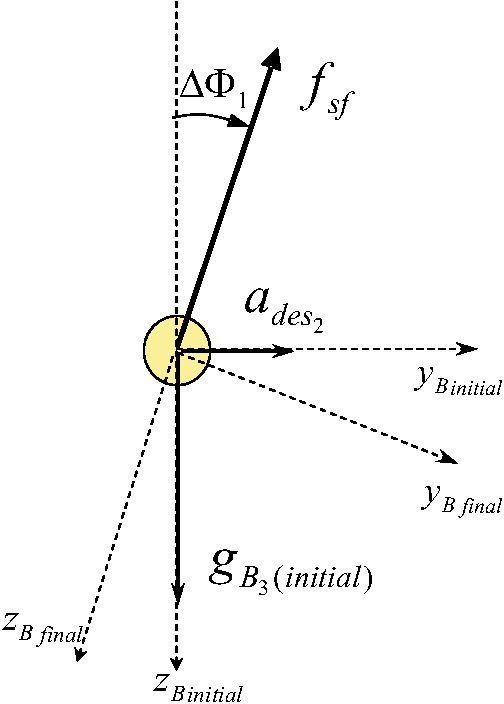
\includegraphics[width=0.4\columnwidth]{pointmass}
%  \centering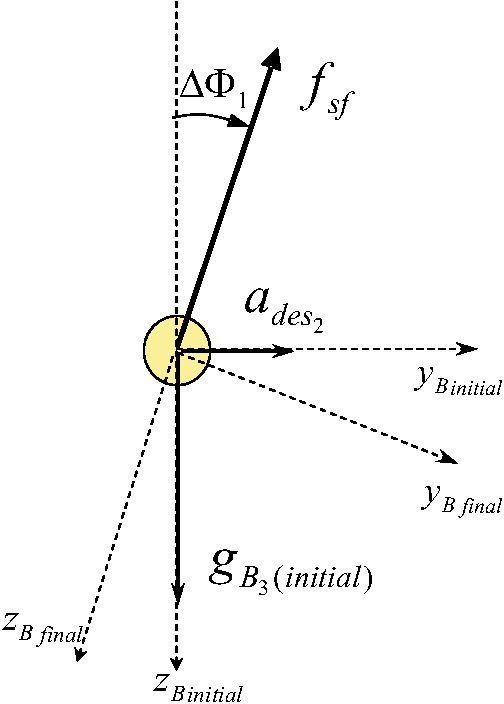
\includegraphics{pointmass}
  \caption{Point mass model for outerloop inversion.}
  \label{f:pointmass}
\end{figure}
%
The translational dynamics may be modeled as a point mass with a
thrust vector that may be oriented in a given direction as
illustrated in \fig{f:pointmass}. More involved inverses
\cite{lipp:mcm:1993} may be used, but the simple relationships between
thrust, attitude and accelerations suffice when used with adaptation
%
\begin{equation}
\label{e:transinverse} \ades =
\begin{bmatrix}
0 \\ 0 \\ Z_{\delta_{coll}}
\end{bmatrix}
\left(
\delta_{coll_{des}} - \delta_{coll_{trim}}
\right)
 + L_{bv}\bfg,
\end{equation}
where, $Z_{\delta_{coll}}$ is the control derivative for
acceleration in the vertical axis. $L_{bv}$ is the direction cosine
matrix that transforms a vector from the vehicle (or local) frame to
the body frame and $\bfg$ is an assumed gravity vector. The desired
specific force along the body $z$ axis may be evaluated as
\[
f_{sf} = (\ades - L_{bv}\bfg)_3.
\]
%
The required collective input may be evaluated as
\[
\delta_{coll_{des}} = \frac{f_{sf}}{Z_{\delta_{coll}}} +
\delta_{coll_{trim}}.
\]
%
The attitude augmentation required in order to orient the thrust
vector to attain the desired translational accelerations are given
by the following small angle corrections from the current
reference body attitude and attitude command
%
\begin{align}
\label{e:DelPhi}
\Delta\Phi_1  = \frac{a_{des_2}}{f_{sf}},\quad%
\Delta\Phi_2  = -\frac{a_{des_1}}{f_{sf}},\quad%
\Delta\Phi_3  = 0,%
\end{align}
For this simplified helicopter model, heading change has no effect
on accelerations in the $x,y$ plane and hence $\Delta\Phi_3 = 0$.
These three correction angles may now be used to generate the
attitude quaternion correction desired by the outer loop. Thus,
%
\begin{equation}
\label{e:qdessmallangle} \qdes =
\bfq(\Delta\Phi_1,\Delta\Phi_2,\Delta\Phi_3),
\end{equation}
where, $\bfq(.)$ is a function\cite{stevens2003} that expresses an
euler-angles-based rotation as a quaternion. The overall detailed
controller architecture is shown in \fig{f:detailarch}.
%

%
\begin{remark}
If the desired specific force $f_{sf}$ is close to zero, which
occurs when the desired acceleration in the body $z$ axis is the
same as the component of gravity vector along that axis, then,
Equation (\ref{e:DelPhi}) is undefined. To overcome this problem,
one can impose a restriction where \sys{e:DelPhi} is only computed
if $| f_{sf}| > \bar{f}_{sf}$, where $\bar{f}_{sf}
> 0$ and is a lower limit. Essentially it means, do not bother
using attitude unless the desired specific force is greater than
$\bar{f}_{sf}$.
\end{remark}
%
%
\subsection{Reference Model}
\label{s:helirefmodel}
Using a linear $\acrm$ and $\alcrm$ in \eq{e:pddrm} and \eq{e:qddrm} results in the following reference model dynamics
\[
\begin{split}
\dot{\bfv}_{r}      &=  R_p(\pc - \prm) + R_d(\vc - \vrm) - \ah\\
\dot{\bfomega}_{r} &= K_p(\tilde{Q}(\qc\oplus\qdes,\qrm)) + K_d(\oc
- \orm) - \alh,
\end{split}
\]
where, $R_p,R_d,K_p,K_d$ are the same gains used for the PD
compensator in \eq{e:pdgains}. If limits on the angular rate or
translational velocities are to be imposed, then they may be easily
included in the reference model dynamics by choosing the following constrained linear reference for $\acrm$ and $\alcrm$.
\begin{align}
\label{e:acrm}
\acrm    &= R_d[\vc - \vrm + \sigma(\inv{R_d}R_p(\pc - \prm), v_{lim})]\\
\label{e:alcrm}
 \alcrm   &= K_d[\oc - \orm +
\sigma(\inv{K_d}K_p\tilde{Q}(\qc\oplus\qdes,\qrm),\omega_{lim})].
\end{align}
This reference model has prescribable aggressiveness, where $\sigma(\cdot)$ is a saturation function and
$v_{lim}$, $\omega_{lim}$ are the translational and angular rate
limits respectively.

\begin{remark}
\label{rem:vlimwlim}Note that there are no limits placed on the
externally commanded position, velocity, angular rate or attitude.
For example, in the translational reference model, if a large
position step is commanded, $\pc = [1000,0,0]^T ft$ and $\vc =
[0,0,0]^T ft/s$, the speed at which this large step will be achieved
is $v_{lim}$. On the other hand if \mbox{$\pc = \int \vc dt$} and
$\vc = [60, 0, 0]^T ft/s$, the speed of the vehicle will be $60
ft/s$. Similarly, $\omega_{lim}$ dictates how fast large attitude
errors will be corrected. Additionally, aggressiveness with which
translational accelerations will be pursued by tilting the body may
be governed by limiting the magnitude of $\qdes$ to the scalar limit
$q_{lim}$.

\begin{comment}
For large $\ades$, the simple form of the outerloop inversion
will result in very large attitude corrections. Hence, the desired
attitude generated by the outerloop, \eq{e:qdessmallangle}, may be
implemented as
\begin{align}
\lambda &= \frac{q_{lim}}{q_{lim} + max(0,\|\Phi\| - q_{lim})}\\
\qdes   &=
q(\lambda\Delta\Phi_1,\lambda\Delta\Phi_2,\lambda\Delta\Phi_3)
\end{align}
where $q_{lim}$ is a limit on the attitude correction and
\mbox{$\|\lambda[\Delta\Phi_1,\Delta\Phi_2,\Delta\Phi_3]^T\| \leq
q_{lim}$}.
\end{comment}
\end{remark}

%
\subsection{Choice of Gains Linear Dynamics}
\label{s:gainchoice} When the combined adaptive inner-outer-loop
controller for position and attitude control is implemented, the
poles for the combined error dynamics must be selected appropriately.
The following analysis applies to the situation where inversion model
error is compensated for accurately by the NN and it is assumed that the
system is exactly feedback linearized. The inner loop and outer loop
each represent a second order system and the resulting position
dynamics $p(s)/p_c(s)$ are fourth order in directions perpendicular
to the rotor spin axis.

When the closed-loop longitudinal dynamics, near hover, are
considered, and with an acknowledgment of an abuse of notation, it
may be written as
\begin{alignat}{3}
\label{eq:xdd}
\ddot{x} &= a_{des} &=
\ddot{x}_c + R_d(\dot{x}_c - \dot{x}) +
R_p(x_c - x)\\
\label{eq:thdd} \ddot{\theta} &= \alpha_{des} &= \ddot{\theta}_g +
K_d(\dot{\theta}_g - \dot{\theta}) + K_p(\theta_g - \theta),
\end{alignat}
where, $R_p$, $R_d$, $K_p$ and $K_d$ are the PD compensator gains
for the inner loop (pitch angle) and outer loop (fore-aft position).
Now $x$ is now the position, $\theta$ the attitude and $\theta_g$
the attitude command. Normally, $\theta_g = \theta_c + \theta_{des}$
where $\theta_c$ is the external command and $\theta_{des}$ the
outer-loop-generated attitude command. Here, it is assumed that the
external attitude command and its derivatives are zero; hence,
$\theta_g = \theta_{des}$. In the following development, the
transfer function $x(s)/x_c(s)$ is found and used to place the poles
of the combined inner-outer loop system in terms of the PD
compensator gains.

When contributions of $\dot{\theta}_g(s)$ and $\ddot{\theta}_g(s)$,
are ignored, the pitch dynamics \eq{eq:thdd} may be rewritten in the
form of a transfer function as
\begin{equation}
\label{eq:thtf} \theta(s) =
\frac{\theta(s)}{\theta_g(s)}\theta_g(s) = \frac{K_p}{s^2 + K_ds +
K_p}\theta_g(s).
%            \cancel{\frac{\theta(s)}{\dot{\theta}_g(s)}\dot{\theta}_g(s)} +
%            \cancel{\frac{\theta(s)}{\ddot{\theta}_g(s)}\ddot{\theta}_g(s)}
\end{equation}
%
If the outer-loop linearizing transformation used to arrive at
\eq{eq:xdd} has the form $\ddot{x} = f\theta$, where $f = -g$ and
$g$ is gravity, it may be written as
\begin{equation}
\label{eq:xtf} s^2x(s) = f\theta(s).
\end{equation}
The outer-loop attitude command may be generated as
\begin{equation}
\label{eq:thol} \theta_{des} = \frac{\ddot{x}_{des}}{f} =
\frac{a_{des}}{f}.
\end{equation}
Note that $\theta_{g} = \theta_{des}$; if $\theta_c = 0$,
\begin{align}
\label{eq:thetag} \theta_g = \theta_{des} &=
\frac{1}{f}\left[\ddot{x}_c + R_d(\dot{x}_c - \dot{x}) +
R_p(x_c-x) \right].
\end{align}
%
When \eq{eq:thtf} and \eq{eq:thetag} are used in \eq{eq:xtf}
\begin{equation}
\begin{split}
\label{eq:s2x}%
s^2x(s) &= \frac{K_p\left[s^2x_c + R_ds(x_c - x) + R_p(x_c - x)
\right]}{s^2 + K_ds + K_p},
\end{split}
\end{equation}
Rearranging the above equation results in the following transfer function
\begin{equation}
\label{eq:xxctf}
\frac{x(s)}{x_c(s)} =
\frac{K_ps^2 + K_pR_ds + K_pR_p}
{s^4 + K_ds^3 + K_ps^2 + K_pR_ds + K_pR_p}.
\end{equation}

One way to choose the gains is by examining a fourth-order
characteristic polynomial written as the product of two second order
systems
\begin{align}
\label{eq:coeffs2}
\Upsilon(s) &= (s^2 + 2\zeta_o\omega_o + \omega_o^2)(s^2 + 2\zeta_i\omega_i + \omega_i^2) \nonumber \\
&=s^4+(2\zeta_i\omega_i+2\zeta_o\omega_o)s^3 \nonumber \\
&+(\omega_i^2+4\zeta_o\omega_o\zeta_i\omega_i+\omega_o^2)s^2 \nonumber \\
&+(2\zeta_o\omega_o\omega_i^2+2\omega_o^2\zeta_i\omega_i)s
+\omega_o^2\omega_i^2,
\end{align}
where, the subscripts $i$, $o$, represent the inner and outerloop
values respectively.

Comparing the coefficients of the poles of \eq{eq:xxctf} and
\eq{eq:coeffs2} allows the gains to be expressed as a function of
the desired pole locations for each axis in turn
\begin{align}
\label{eq:gains2}
R_p &= \frac{\omega_o^2\omega_i^2}{\omega_i^2+4\zeta_o\omega_o\zeta_i\omega_i+\omega_o^2} \nonumber \\
R_d &=
2\frac{\omega_o\omega_i(\zeta_o\omega_i+\omega_o\zeta_i)}{\omega_i^2+4\zeta_o\omega_o\zeta_i\omega_i+\omega_o^2}
\nonumber \\
K_p &= \omega_i^2+4\zeta_o\omega_o\zeta_i\omega_i+\omega_o^2 \nonumber \\
K_d &= 2\zeta_i\omega_i+2\zeta_o\omega_o.
\end{align}
Additionally, the zeros of the transfer function given by
\eq{eq:xxctf} affect the transient response. Thus, $\omega_i,
\zeta_i,\omega_o, \zeta_o$ must be selected such that performance is
acceptable.
%
\subsection{Imposing Response Characteristics}
\label{r:performancemetrics}The methods presented in this chapter do
not contain assumptions that limit its application to unmanned
helicopters. Manned rotorcraft normally have to meet standards, such
as those specified in the Aeronautical Design Standard-33
\cite{ads33e} handling qualities specifications. Control system
performance\cite{civita:gnc:02,rysdyk:itcst:2005} may be evaluated by
imposing response requirements and computing metrics prescribed in
the ADS-33. When there is no saturation, the hedging signals
$\ah,\alh$ are zero. When it is assumed that the adaptation has
reached its ideal values of $(V^*,W^*)$, then
\[
\begin{split}
\vd &= \acrm + \apd + \bfepsilon_a\nonumber \\
\od &= \alcrm + \alpd + \bfepsilon_{\alpha},
\end{split}
\]
where $\bfepsilon_a$ and $\bfepsilon_{\alpha}$ are bounded by
$\bar{\epsilon}$. Additionally, the Lyapunov analysis provides
guaranteed model following, which implies $\apd$ and $\alpd$ are
small. Thus, $\vd \approx \acrm$ and $\od \approx \alcrm$. Hence, as
long as the preceding assumptions are valid over the bandwidth of
interest, the desired response characteristics may be encoded into
the reference model $\acrm$ and $\alcrm$.
%





\newlength{\myfigheight}% subfigure width
\newlength{\mytfigheight}% subfigure width
%\setlength{\myfigheight}{0.19\textheight}
\setlength{\myfigheight}{0.40\textheight}
\setlength{\mytfigheight}{0.33\textheight}

\newlength{\subfigwidth}% subfigure width
\newlength{\subfigcolsep}% separation between subfigures
\setlength{\subfigcolsep}{2\tabcolsep}% tie to that used for tabular
\section{Experimental Results}
\todo{I would fix sizes of figures, but I think that the typesetters will do that, I think they prefer all figures at the end, full size.}
\label{c:results}

The proposed guidance and control architecture was applied to the
Georgia Institute of Technology Yamaha R-Max helicopter (GTMax)
shown in \fig{f:helipic}. The GTMax helicopter weighs about $157 lb$
and has a main rotor radius of $5.05 ft$. Nominal rotor speed is
$850$ revolutions per minute. Its practical payload capability is
about $66 lbs$ with a flight endurance of greater than 60 minutes.
It is also equipped with a Bell-Hillier stabilizer bar. Its avionics
package includes a Pentium 266 flight control computer, an inertial
measurement unit (IMU), a global positioning system, a 3-axis
magnetometer and a sonar altimeter. The control laws presented in
this chapter were first implemented in
simulation~\cite{kannan:mst:2004} using a nonlinear helicopter model
that included flapping and stabilizer bar dynamics. Wind and gust
models were also included. Additionally, models of sensors with
associated noise characteristics were implemented. Many aspects of
hardware such as the output of sensor model data as serial packets
was simulated. This introduced digitization errors as would exist in
real-life and also allowed testing of many flight specific
components such as sensor drivers. The
navigation system~\cite{henrik:jacic:2006} consists of a 17-state Kalman filter to estimate
variables such as attitude, and terrain altitude. The navigation
filter was executed at $100 Hz$ and corresponds to the highest rate
at which the IMU is able to provide data. Controller calculations
occurred at $50 Hz$. The control laws were first implemented as
C-code and tested in simulation. Because almost all aspects specific
to flight-testing were included in the simulation environment, a
subset of the code from the simulation environment was implemented
on the main flight computer. During flight, ethernet and
serial-based data links provided a link to the ground station
computer that allowed monitoring and uploading of way-points. A
simple kinematics-based trajectory generator (with limits on
accelerations) was used to generate smooth consistent trajectories
($\pc,\vc,\qc,\oc$) for the controller. Various moderately
aggressive maneuvers were performed during flight to test the
performance of the trajectory-tracking controller. Controller
testing began with simple hover followed by step responses and
way-point navigation. Following initial flight tests, aggressiveness
of the trajectory was increased by relaxing acceleration limits in
the trajectory generator and relaxing $\omega_{lim}$ and $v_{lim}$
in the reference models. Tracking error performance was increased by
increasing the desired bandwidth of the controllers. Selected
results from these flight tests are provided in the following
sections.

\subsection{Parameter Selections}
The controller parameters for the inner loop involved choosing $K_p,
K_d$ based on a natural frequency of $2.5, 2, 3\ rad/s$ for the
roll, pitch and yaw channels respectively and damping ratio of
$1.0$. For the outer loop, $R_p, R_d$ were chosen based on a natural
frequency of $2, 2.5, 3\ rad/s$ for the x, y and z body axis all
with a damping ratio of unity. The NN was chosen to have 5 hidden
layer neurons. The inputs to the network included body axis
velocities and rates as well as the estimated pseudocontrols i.e,
$\bfx_{in} = [\bfv_B^T, \bfomega_B^T, \ahat^T, \alhat^T]$. The
output layer learning rates $\Gamma_W$ were
set to unity for all channels and a learning rate of $\Gamma_V = 10$
was set for all inputs. Limits on maximum translation rate and
angular rate in the reference model dynamics were set to $v_{lim} =
10\ ft/s$ and $\omega_{lim} = 2\ rad/s$. Additionally, attitude
corrections from the outer loop, $\qdes$ were limited to $30$
degrees.

\label{r:actuatorlimits}With regard to actuator magnitude limits,
the helicopter has a radio-control transmitter that the pilot may
use to fly the vehicle manually. The full deflections available on
the transmitter sticks in each of the channels were mapped as
$\delta_{lat},\delta_{lon},\delta_{ped} \in [-1,1]$ corresponding to
the full range of lateral tilt and longitudinal tilt of the swash
plate and full range of tail rotor blade pitch. The collective was
mapped as $\delta_{coll} \in [-2.5,1]$, corresponding to the full
range of main rotor blade pitch available to the human pilot. The
dynamic characteristics of the actuators were not investigated in
detail. Instead, conservative rate limits were artificially imposed
in software. Noting that $\bfdelta =
[\delta_{coll},\delta_{lat},\delta_{lon},\delta_{ped}]^T$, the
actuator model used for PCH purposes as well as artificially
limiting the controller output has form
\begin{equation}
\label{e:ghatcontinuous} \dot{\hat{\bfdelta}} = \lim_{\lambda
\rightarrow +\infty} \sigma\left(\lambda(\sigma(\deldes,
\delmin,\delmax) - \hat{\bfdelta}),\deldmin,\deldmax \right),
\end{equation}
where $\hat{\bfdelta}$ is limited to lie in the interval
$[\delmin,\delmax]$. The discrete implementation has the form
\begin{equation}
\label{e:ghatdiscrete}
\begin{split}
\hat{\bfdelta}&[k+1] = \sigma\left(\hat{\bfdelta}[k] +
\sigma\left(\sigma(\deldes,\delmin,\delmax) -
\hat{\bfdelta}[k],\Delta T\deldmin,\Delta T\deldmax\right), \delmin,
\delmax\right),
\end{split}
\end{equation}
where $\Delta T$ is the sampling time. The magnitude limits were set
to
\begin{align}
\label{e:magnitudelimits}
\delmin &= [-2.5,-1,-1,-1]^T \nonumber\\
\delmax &= [1,1,1,1]^T
\end{align}
units, and the rate limits were set to
\begin{align}
\label{e:ratelimits}
\deldmin &= [-4,-2,-2,-2]^T\nonumber\\
\deldmax &= [4,2,2,2]^T
\end{align}
units per second.

%\subsection{Simulation}
%The helicopter was commanded to perform a circular maneuver in the
%North-East plane with constant altitude. Constant speed was
%commanded around the circuit at the same time commanding heading
%by declaring the number of pirouettes to be performed per loop.
%The trajectory equations are given by
%\begin{alignat}{2}
%p_c &=
%\begin{bmatrix}
%\frac{V}{\omega}\cos(\omega t) \\
%\frac{V}{\omega}\sin(\omega t) \\
%-h
%\end{bmatrix},
%\qquad v_c &=
%\begin{bmatrix}
%-V\sin(\omega t) \\
%V\cos(\omega t) \\
%0
%\end{bmatrix} \nonumber \\
%\psi_c &= \omega t f
%\end{alignat}
%where, $t$ is simulation time and $h$ is a constant altitude
%command. $V$ is speed of the maneuver, $\omega$ is angular speed
%of the helicopter around the local frame origin, and $f$ is number
%of pirouettes to be performed per circuit. If $\omega = \pi/2\
%rad/s$, the helicopter will go around once every 4 seconds. If
%$f=1$, the helicopter will rotate once every revolution.
%
%Maneuver parameters involved setting the speed of the maneuver to
%$V=10\ ft/s$, $\omega = 0.5\ rad/s$ and frequency of pirouette to
%once every revolution i.e., $f = 1$. Simulation with the above
%parameters were performed with and without outerloop adaptation.
%Innerloop adaptation was enabled in all cases. \fig{f:iladnorth}
%shows the position tracking in the x-axis of the local frame
%(North). \fig{f:iladxypartialtime} illustrates the position plot
%of the helicopter in the x-y plane during the first 30 seconds of
%simulation and the latter 80-100 seconds of simulation at which
%point the innerloop may be assumed to be fully trained. Tracking
%without adaptation in the outerloop is quite poor due to the
%simplistic point-mass model used for outerloop inversion.
%\begin{figure}
%  \centering\includegraphics{iladnorth}
%  \caption{North Position with innerloop adaptation only}
%  \label{f:iladnorth}
%\end{figure}
%
%\begin{figure}
%  \centering\includegraphics{iladxypartialtime}
%  \caption{x-y plane trajectory plot of helicopter position with innerloop adaptation only}
%  \label{f:iladxypartialtime}
%\end{figure}
%
%
%\begin{figure}
%  \centering\includegraphics{fulladnorth}
%  \caption{North Position with both inner and outer loop adaptation}
%  \label{f:fulladnorth}
%\end{figure}
%
%\begin{figure}
%  \centering\includegraphics{fulladxypartialtime}
%  \caption{x-y plane trajectory plot of helicopter position with both inner and outerloop adaptation}
%  \label{f:fulladxypartialtime}
%\end{figure}
%
%
%\begin{figure}
%  \centering\includegraphics{fulladpsi}
%  \caption{Heading command and response for inner and outer loop adaptation case}
%  \label{f:fulladpsi}
%\end{figure}
%
%\fig{f:fulladnorth} and \fig{f:fulladxypartialtime} shows similar
%plots but with adaptation in both the inner and outer loops. The
%network is able to compensate for approximations in both the
%innerloop dynamics and the outerloop dynamics. In
%\fig{f:fulladxypartialtime}, during the latter parts of the
%simulation, the network appears to be fully trained with accurate
%tracking to within 2 ft. Additionally, \fig{f:fulladpsi}
%illustrates the heading command and response of the helicopter for
%the full adaptation case.
%
%
%%print(gcf,'-dpsc','landingAltitude');
%%print(gcf,'-dpsc','landingColl');
%%print(gcf,'-dpsc','takeoffAlt');
%%print(gcf,'-dpsc','takeoffColl');
%%print(gcf,'-dpsc','headingStep');
%%print(gcf,'-dpsc','headingStepPed');
%%print(gcf,'-dpsc','nsStep');
%%print(gcf,'-dpsc','ewStep');
%%print(gcf,'-dpsc','highspeed');
%%print(gcf,'-dpsc','forwardflight');
%%print(gcf,'-dpsc','pir');
%%print(gcf,'-dpsc','pirHeading');
%%print(gcf,'-dpsc','pirControls');

\subsection{Flight Test}


\begin{figure}
  \begin{center}
  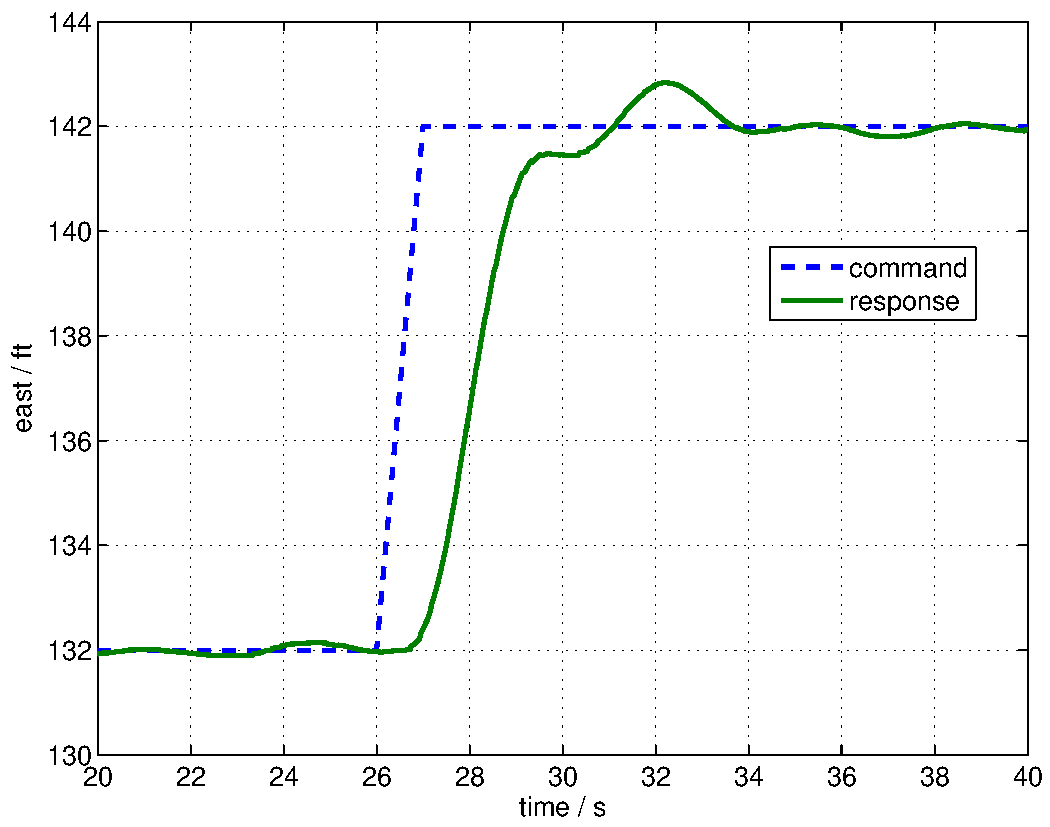
\includegraphics[height=\myfigheight]{ewStep}
  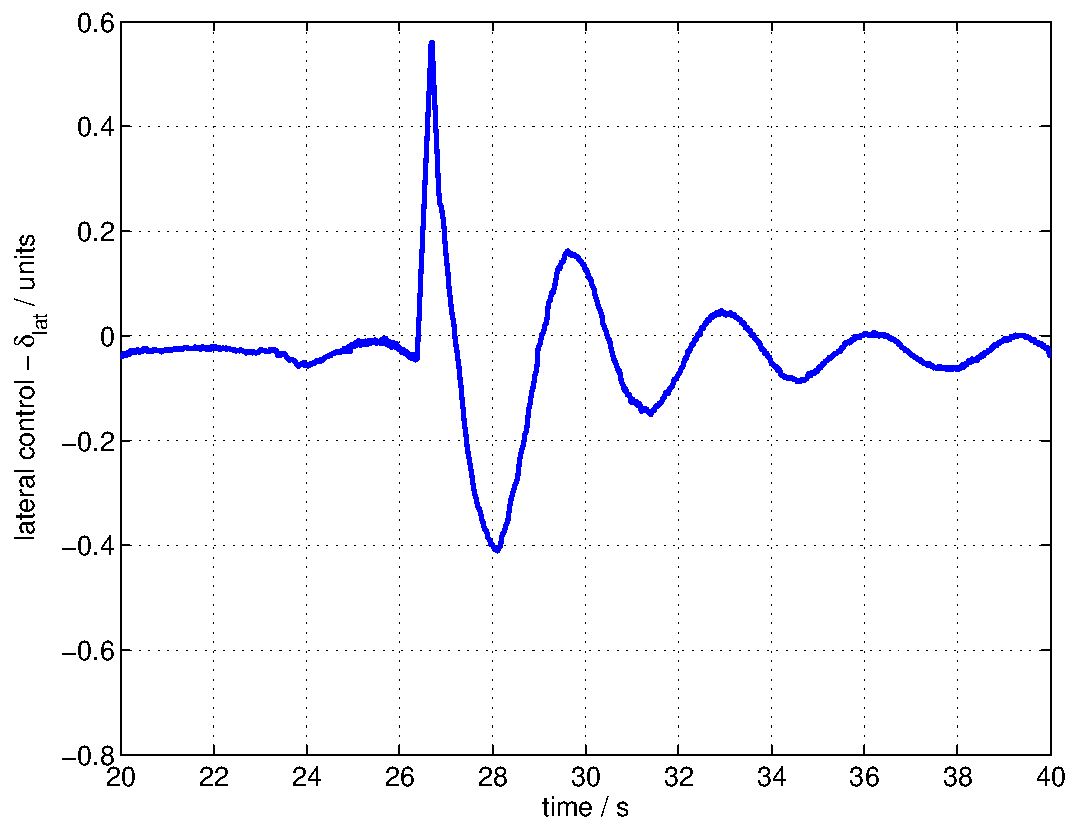
\includegraphics[height=\myfigheight]{ewStepLat}
  \caption{Response to a $20 ft$ step in the lateral direction.}
  \label{f:ewStep}
  \end{center}
\end{figure}
%
\begin{figure}
  \begin{center}
  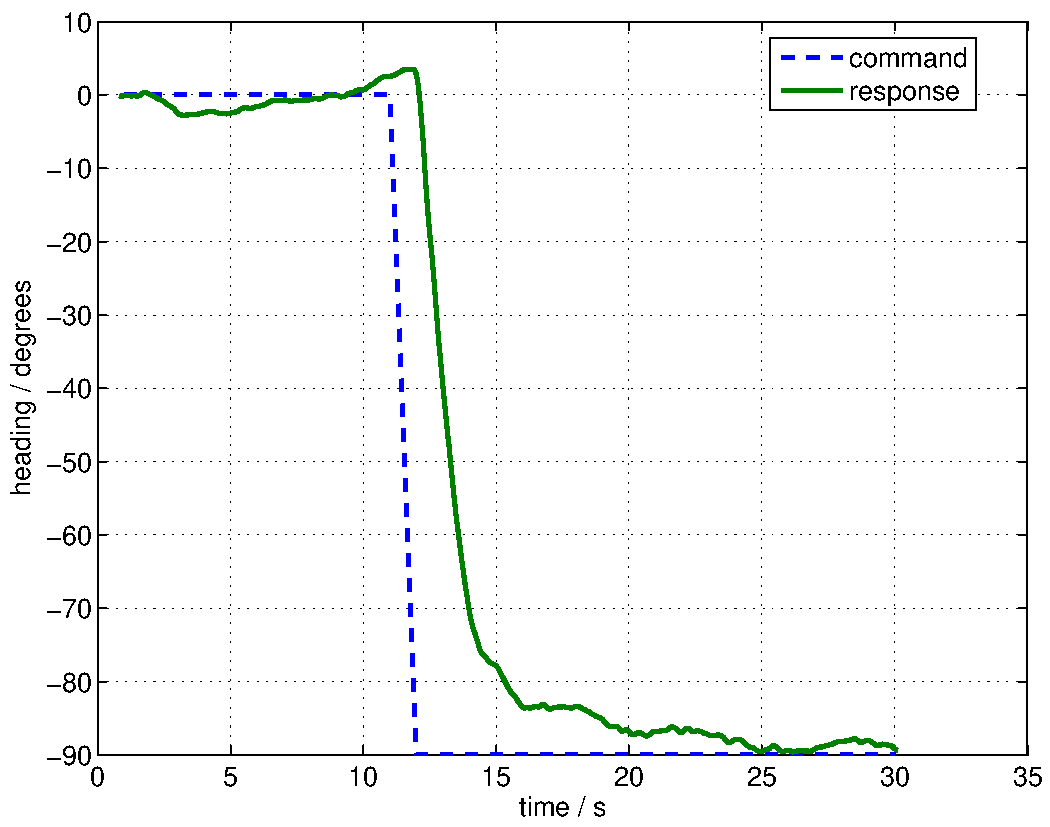
\includegraphics[height=\myfigheight]{headingStep}
  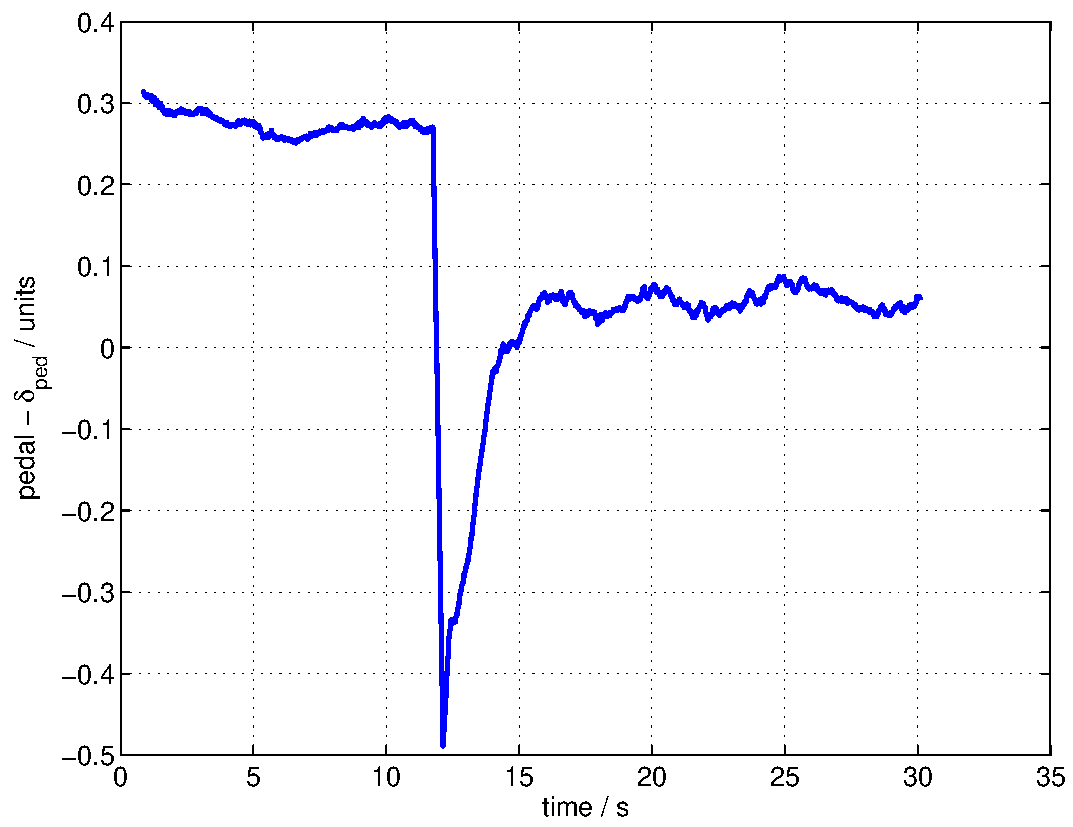
\includegraphics[height=\myfigheight]{headingStepPed}
  \caption{Response to a 90 degree heading command.}
  \label{f:headingStep}
  \end{center}
\end{figure}
Finally, the controller was flight tested on the GTMax helicopter
shown in \fig{f:helipic}. A lateral position step response is shown
in \fig{f:ewStep}.  The vehicle heading was regulated due-north
during this maneuver. Lateral control deflections during the
maneuver were recorded and are also shown. A step heading command
response and pedal control history is shown in \fig{f:headingStep}. It should be noted that during
flight tests, states were sampled at varying rates in order to
conserve memory and datalink bandwidth. The trajectory commands
$\pc,\vc,\qc,\oc$ were sampled at $1 Hz$, actuator deflections
$\delta_{coll},\delta_{lon},\delta_{lat}$ and $\delta_{ped}$ were
sampled at $50 Hz$, vehicle position and speed was sampled at $50
Hz$. Since the command vector is sampled at a low rate ($1 Hz$), a
step command appears as a fast ramp in figures.

\begin{figure}
  \begin{center}
  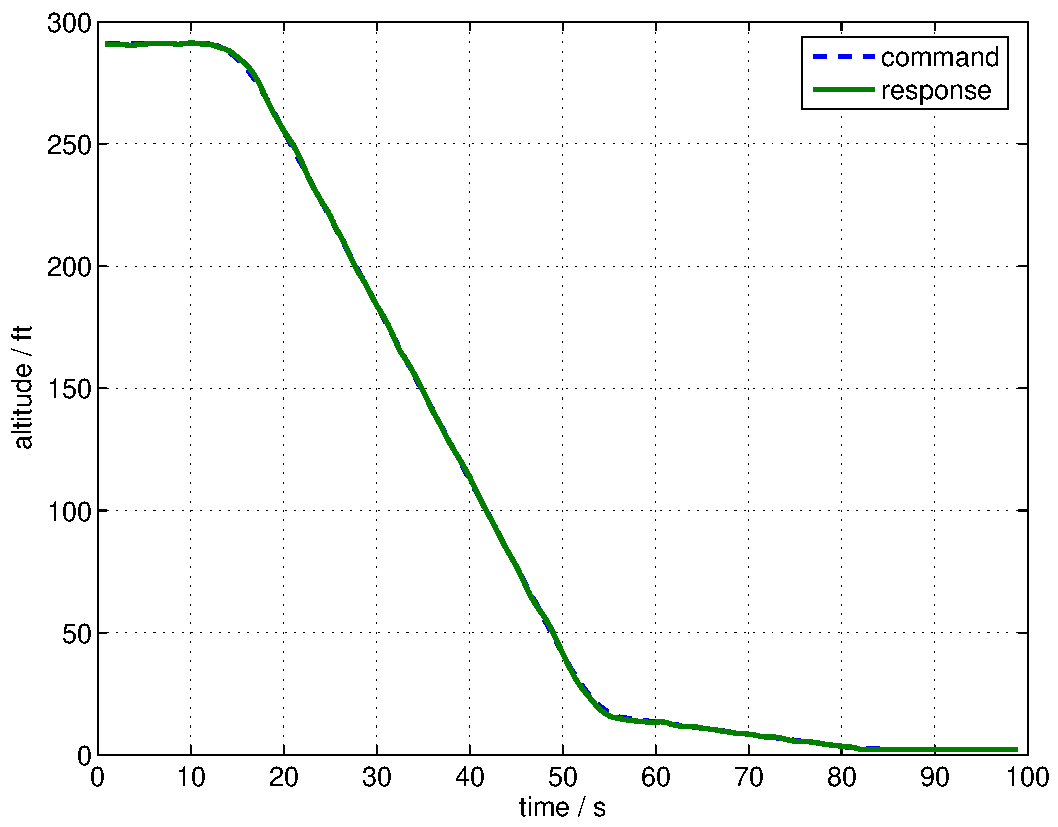
\includegraphics[height=\myfigheight]{landingAlt}
  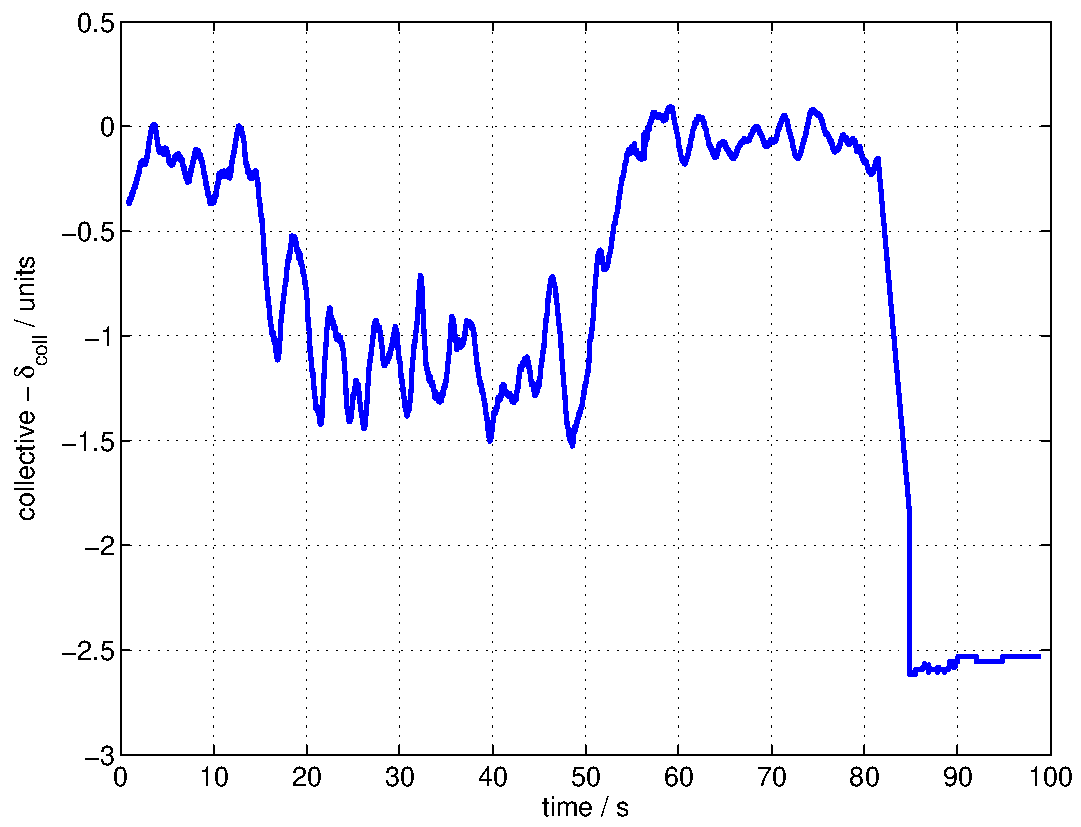
\includegraphics[height=\myfigheight]{landingColl}
  \caption{Automatic landing maneuver.}
  \label{f:landing}
  \end{center}
\end{figure}
%
\begin{figure}
  \begin{center}
  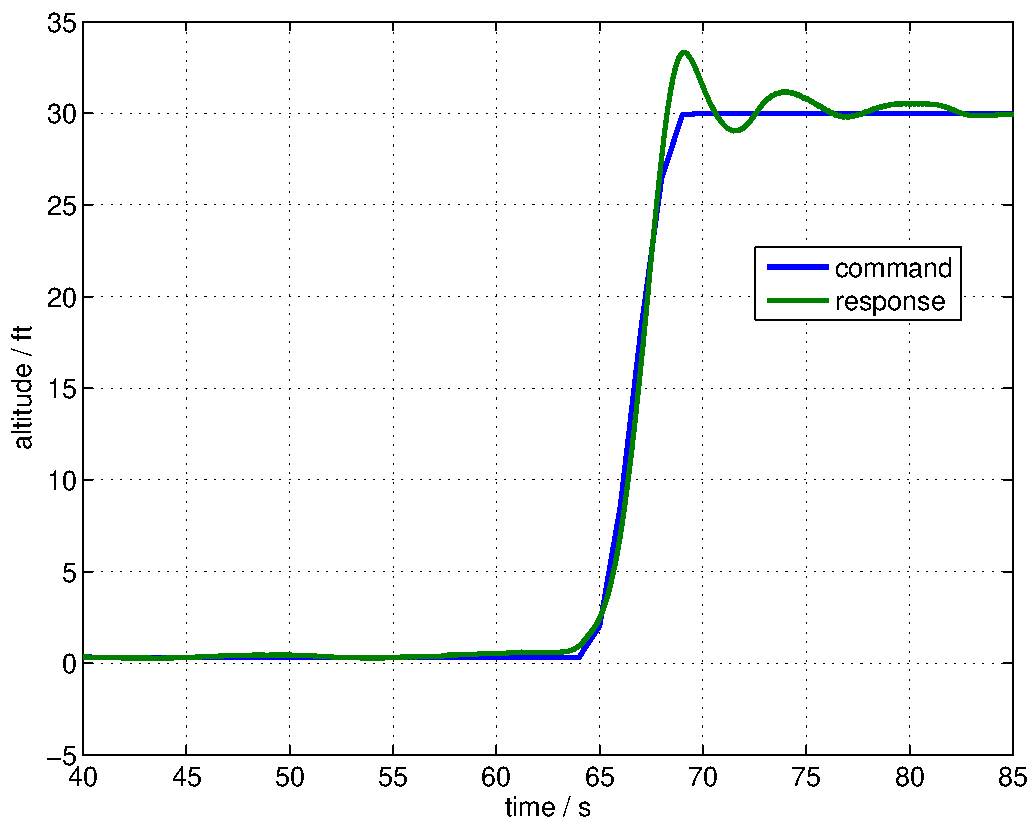
\includegraphics[height=\myfigheight]{takeoffAlt}
  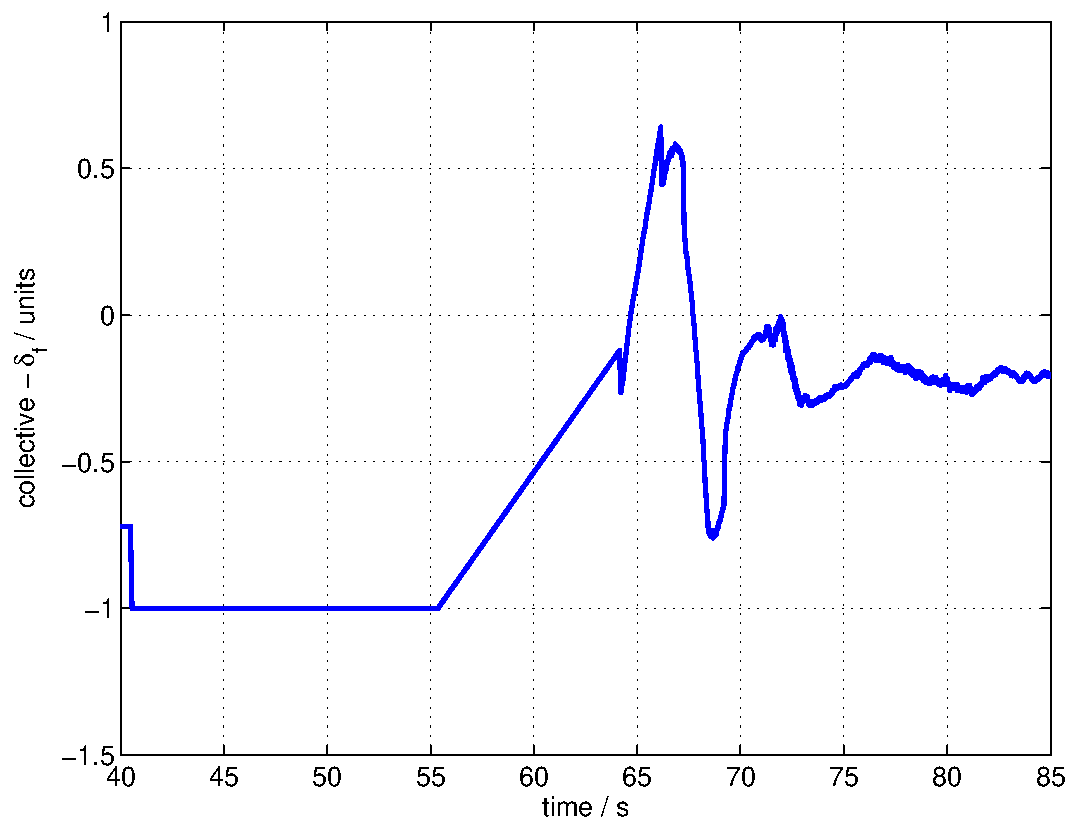
\includegraphics[height=\myfigheight]{takeoffColl}
  \caption{Automatic take-off maneuver.}
  \label{f:takeoff}
  \end{center}
\end{figure}

During takeoff and landing phases a range sensor (sonar) is used to
maintain and update the estimated local terrain altitude in the
navigation system. The sonar is valid up to $8 ft$ above the
terrain, sufficient for landing and takeoff purposes.
\fig{f:landing} illustrates the altitude and collective profile
during a landing. The vehicle starts at an initial hover at $300
ft$, followed by a descent at $7 ft/s$ until the vehicle is $15 ft$
above the estimated terrain. The vehicle then descends at $0.5 ft/s$
until weight-on-skids is automatically detected at which point the
collective is slowly ramped down. Automatic takeoff
(\fig{f:takeoff}) is similar where the collective is slowly ramped
up until weight-on-skids is no longer detected. It should be noted
that NN adaptation is active at all times except when
weight-on-skids is active. Additionally, when weight is on skids,
the collective ramp-up during takeoff and ramp-down during landing
is open-loop.


\begin{figure}
  \begin{center}
%  \subfigure[\label{f:highspeedPos}]{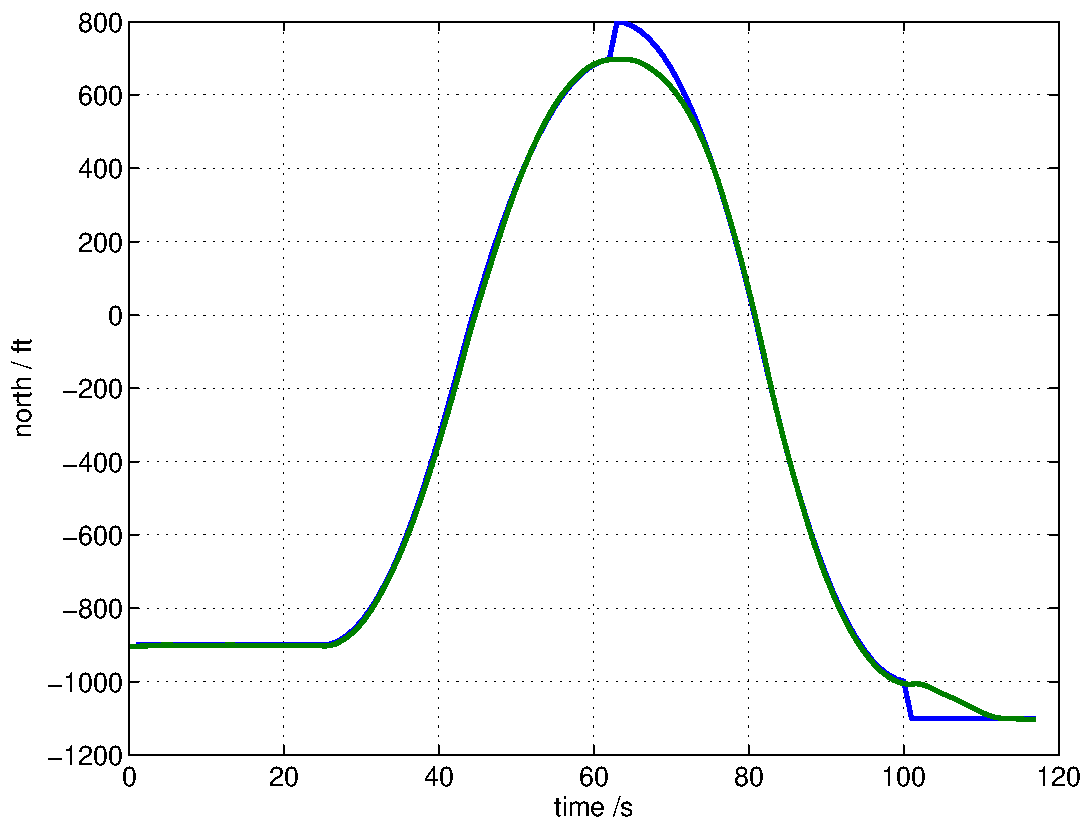
\includegraphics[height=\myfigheight]{highspeedPos}}
  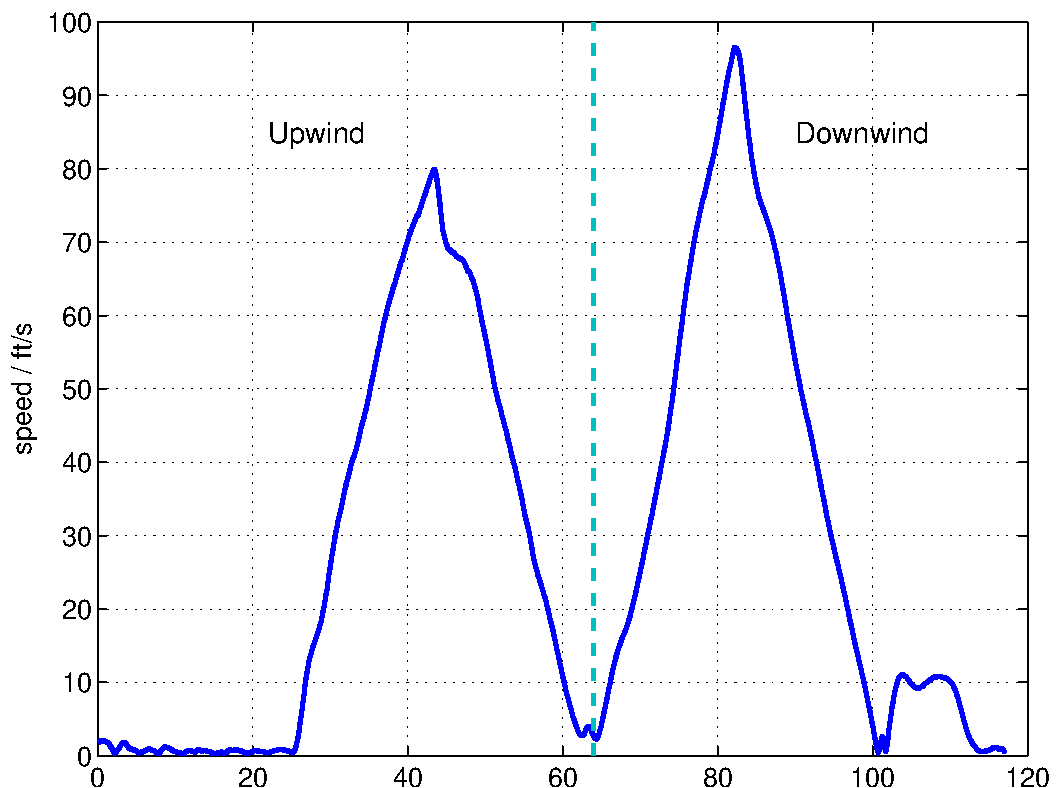
\includegraphics[height=\mytfigheight]{highspeedSpeed}
  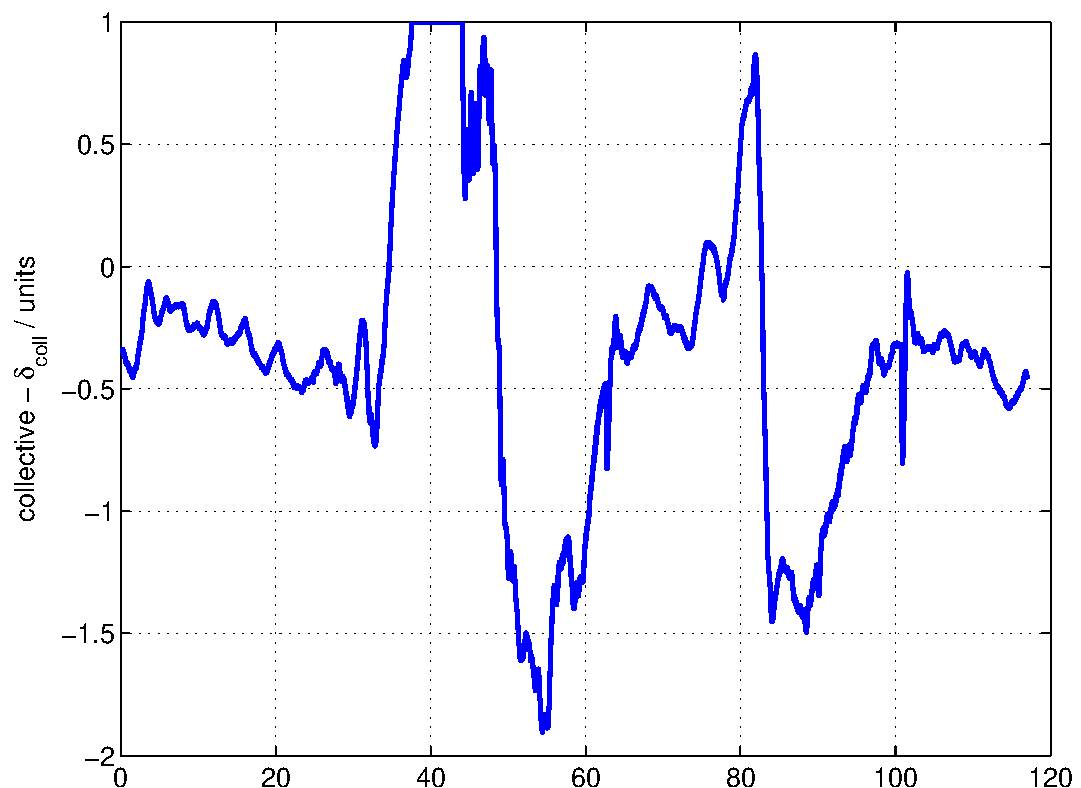
\includegraphics[height=\mytfigheight]{highspeedColl}
  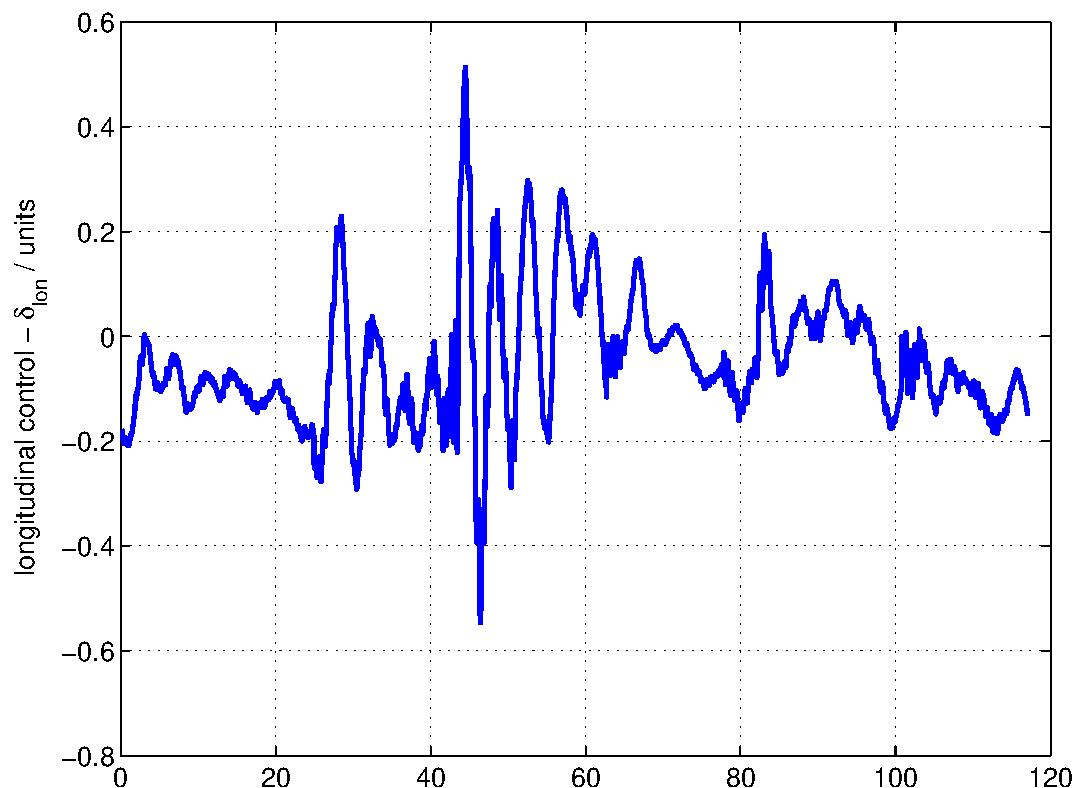
\includegraphics[height=\mytfigheight]{highspeedLong}
  \caption{High speed forward flight up to $97 ft/s$.}
  \label{f:highspeed}
  \end{center}
\end{figure}
\begin{figure}
  \begin{center}
  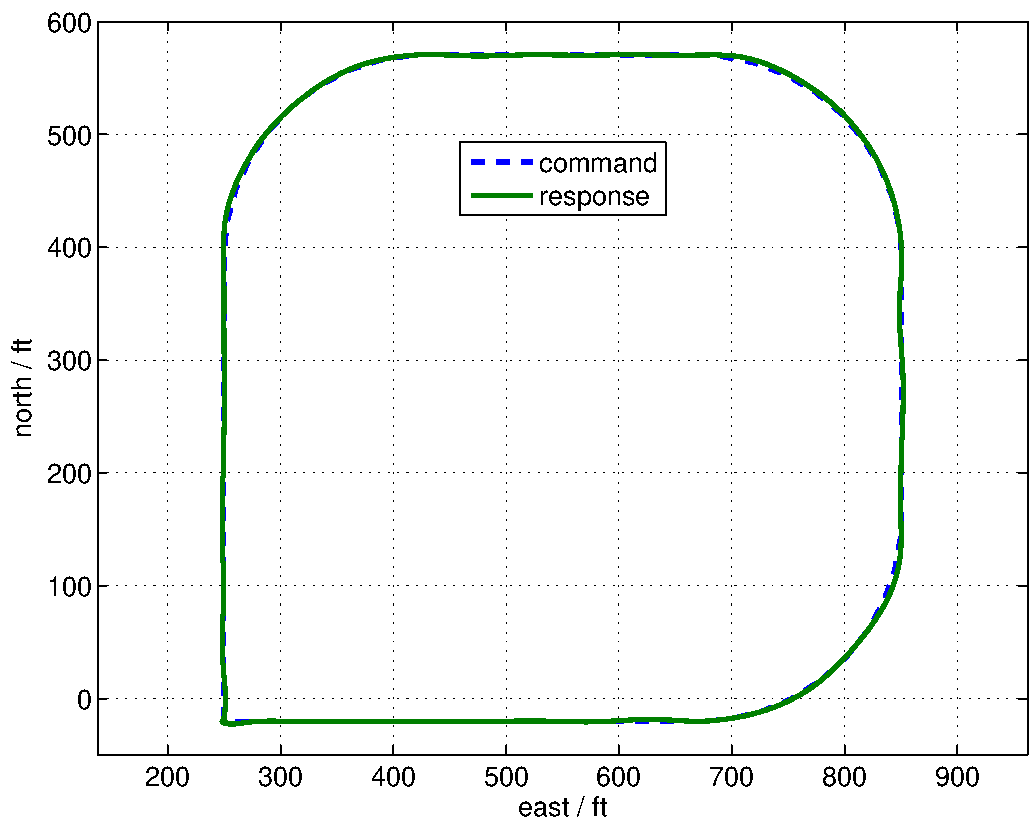
\includegraphics[height=\myfigheight]{squareNorthEast}
  \caption{Flying a square pattern at $30 ft/s$.}
  \label{f:squareNorthEast}
  \end{center}
\end{figure}
\begin{figure}
  \begin{center}
  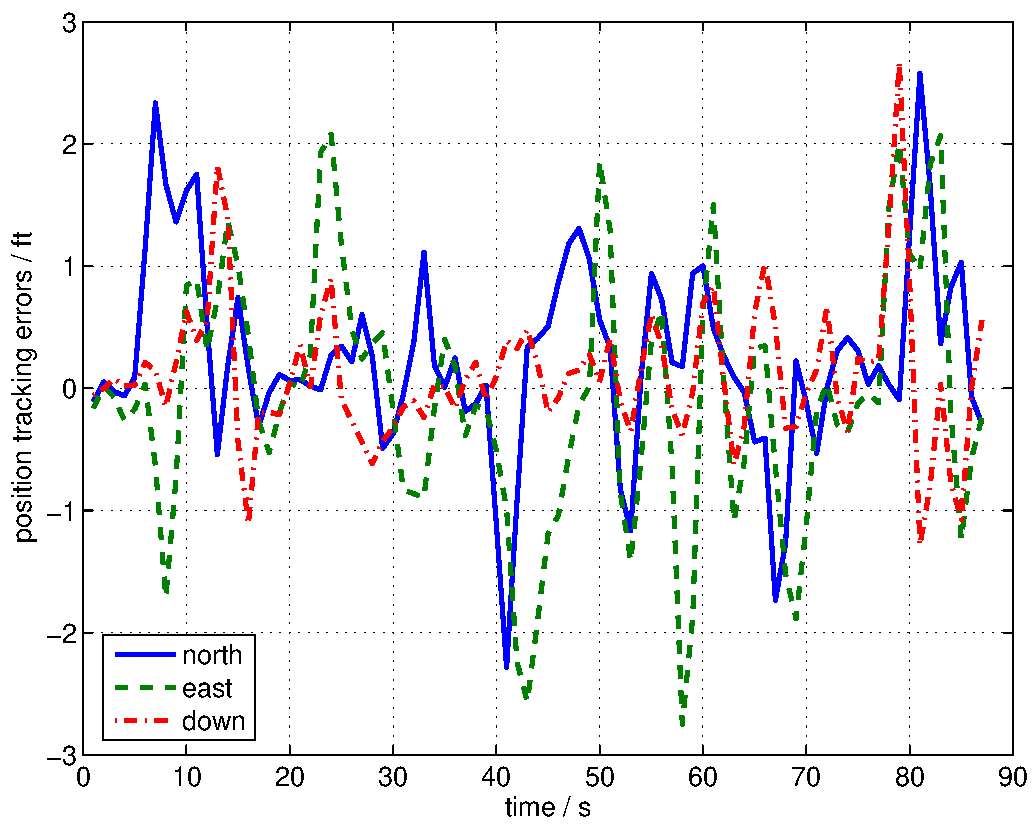
\includegraphics[height=\myfigheight]{squarePosError}
  \caption{Command tracking errors while flying a square pattern at $30 ft/s$.}
  \label{f:squarePosError}
  \end{center}
\end{figure}

The approximate model used to compute the dynamic inverse
(\eq{e:transinverse} and \eq{e:attinverse}) is based on a linear
model of the dynamics in hover. To evaluate controller performance
at different points of the envelope, the vehicle was commanded to
track a trajectory that accelerated up to a speed of $100 ft/s$. To
account for wind, an upwind and downwind leg were flown. In the
upwind leg the vehicle accelerated up to $80 ft/s$ and during the
downwind leg the vehicle accelerated up to a speed of $97 ft/s$ as
shown in \fig{f:highspeed}. Collective and longitudinal control
deflections are also shown. In the upwind leg, the collective is
saturated and the vehicle is unable to accelerate further. The
longitudinal control deflections behave nominally as the vehicle
accelerates and decelerates through a wide range of the envelope.
The NN is able to adapt to rapidly changing flight conditions, from
the baseline inverting design at hover through to the maximum speed
of the aircraft. A conventional proportional-integral-derivative
design would have required scheduling of gains throughout the speed
range. More significantly, classical design would require accurate
models at each point, unlike this design which does not. In addition
to flight at high speeds, tracking performance was evaluated at
moderate speeds, where a square pattern was flown at $30 ft/s$ for
which position tracking is shown in \fig{f:squareNorthEast}.
External command position tracking errors are shown in
\fig{f:squarePosError} with a peak total position error $3.3 ft$ and
standard deviation of $0.8 ft$.

\begin{figure}
  \begin{center}
  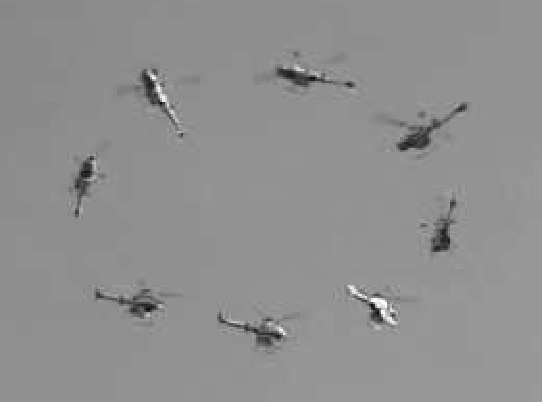
\includegraphics[height=\myfigheight]{pir15m1}
  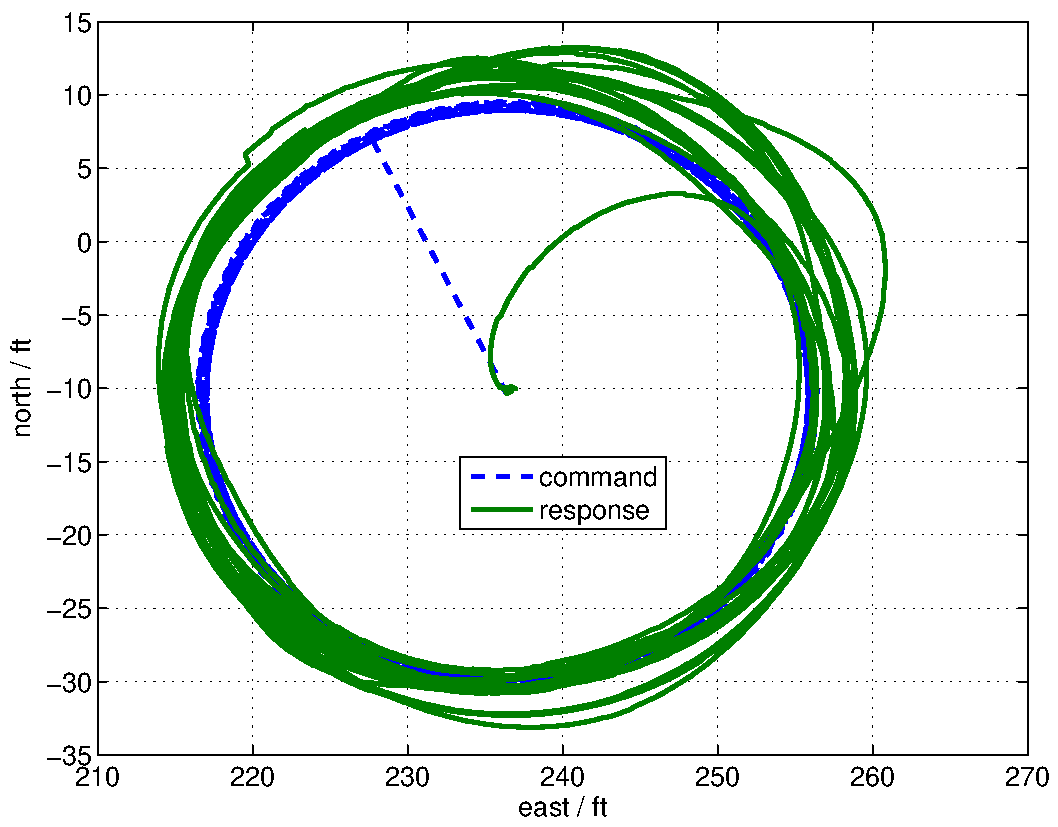
\includegraphics[height=\myfigheight]{pir}
  \caption{Circular maneuver, with 360\textdegree\ heading changes during the circuit.}
  \label{f:pirPosition}
  \end{center}
\end{figure}

\begin{figure}
  \begin{center}
  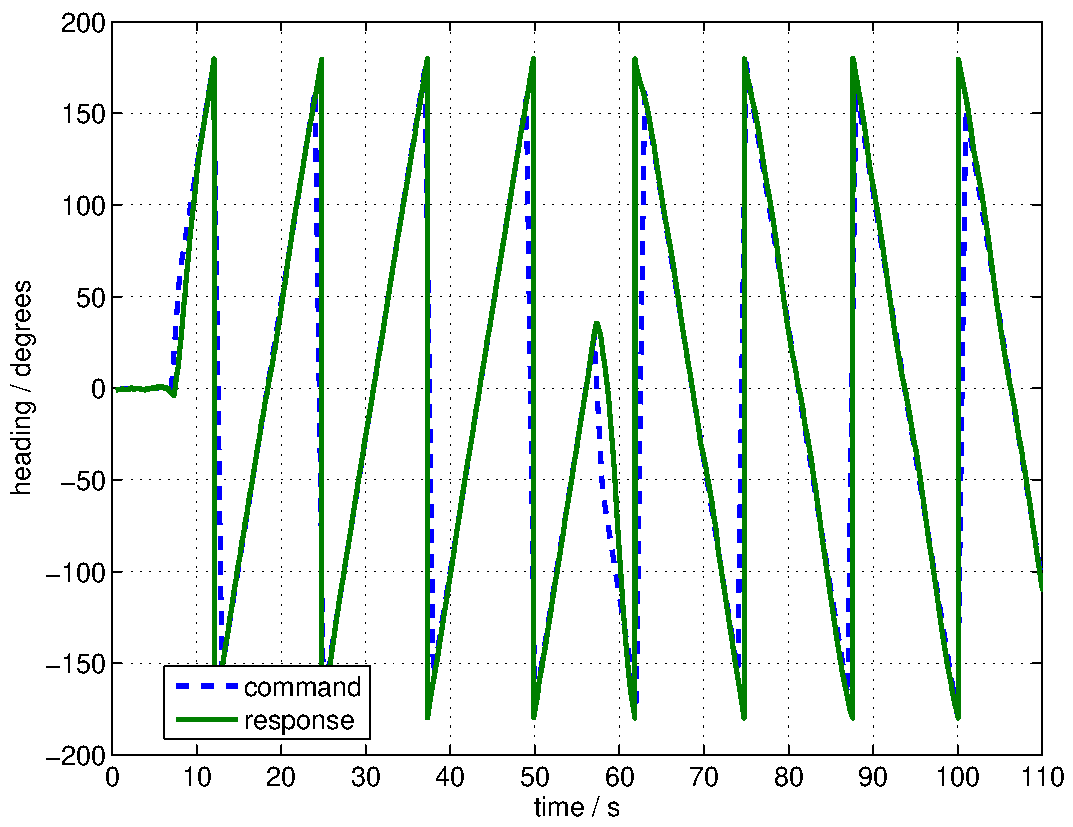
\includegraphics[height=\myfigheight]{pirHeading}
  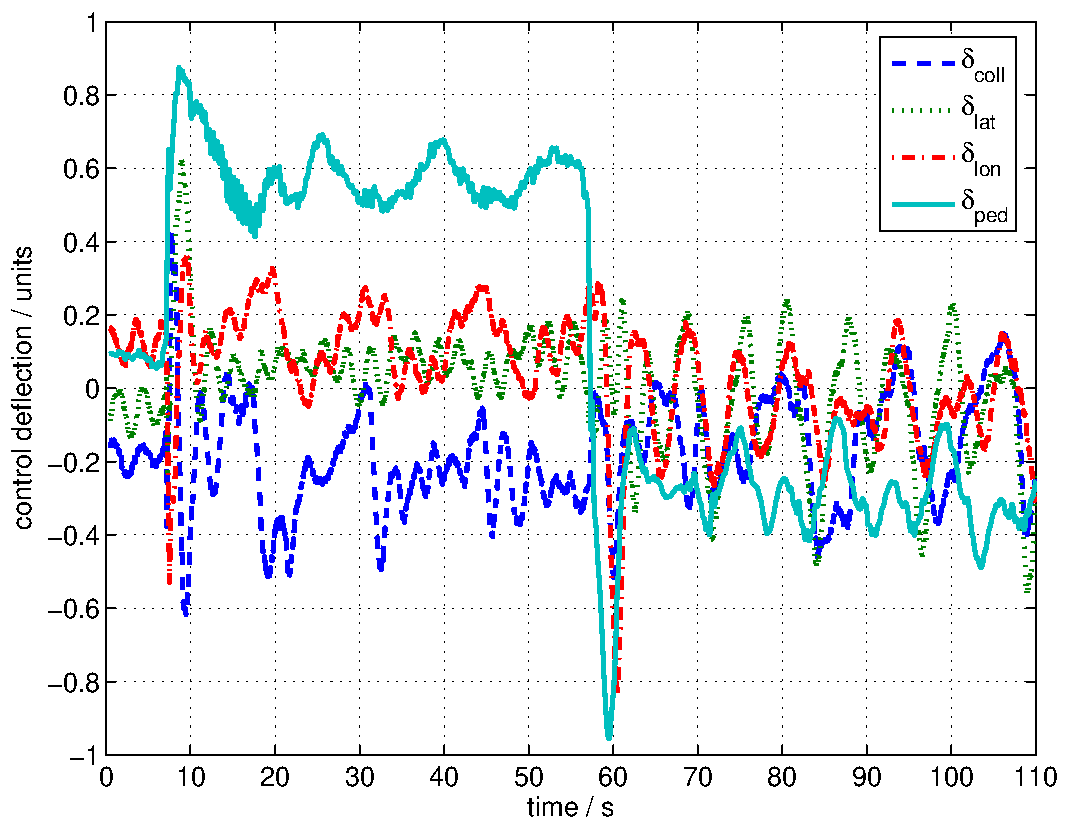
\includegraphics[height=\myfigheight]{pirControls}
  \caption{Heading tracking during circular maneuver and control time history.}
  \label{f:pirHeading}
  \end{center}
\end{figure}

Many maneuvers such as high-speed flight are quasi steady, in the
sense that once in the maneuver, control deflection changes are only
necessary for disturbance rejection. To evaluate performance where
the controls have to vary significantly in order to track the
commanded trajectory, the helicopter was commanded to perform a
circular maneuver in the north-east plane with constant altitude and
a constantly changing heading. The trajectory equations for this
maneuver are given by
\begin{alignat*}{2}
\pc &=
\begin{bmatrix}
\frac{V}{\omega}\cos(\omega t) \\
\frac{V}{\omega}\sin(\omega t) \\
-h
\end{bmatrix},
\qquad \vc &=
\begin{bmatrix}
-V\sin(\omega t) \\
V\cos(\omega t) \\
0
\end{bmatrix}, \nonumber \\
\psi_c &= \omega t f,
\end{alignat*}
where, $t$ is current time and $h$ is a constant altitude command.
$V$ is speed of the maneuver, $\omega$ is angular speed of the
helicopter around the maneuver origin, and $f$ is number of
360\textdegree\ changes in heading to be performed per circuit. If
$\omega=\pi/2 rad/s$, the helicopter will complete the circular
circuit once every 4 seconds. If $f = 1$, the helicopter will rotate
anticlockwise 360\textdegree\ once per circuit. \fig{f:pirPosition}
shows the response to such a trajectory with parameters $\omega =
0.5 rad/s$, $f = 1$, $V = 10 ft/s$. After the initial transition
into the circular maneuver, the tracking is seen to be within 5 ft.
To visualize the maneuver easily, superimposed still images of the
vehicle during the circular maneuver are shown. Both anticlockwise
and clockwise heading changes during the maneuver were tested by
changing the parameter from $f=1$ (anticlockwise) to $f = -1$
(clockwise) at $t = 55s$. \fig{f:pirHeading} shows that heading
tracking is good in both cases. The time history of the pedal input
$\delta_{ped}$ and all other controls during the maneuver is also
shown and illustrates how the vehicle has to exercise all of its
controls during this maneuver.

\begin{figure}
  \begin{center}
  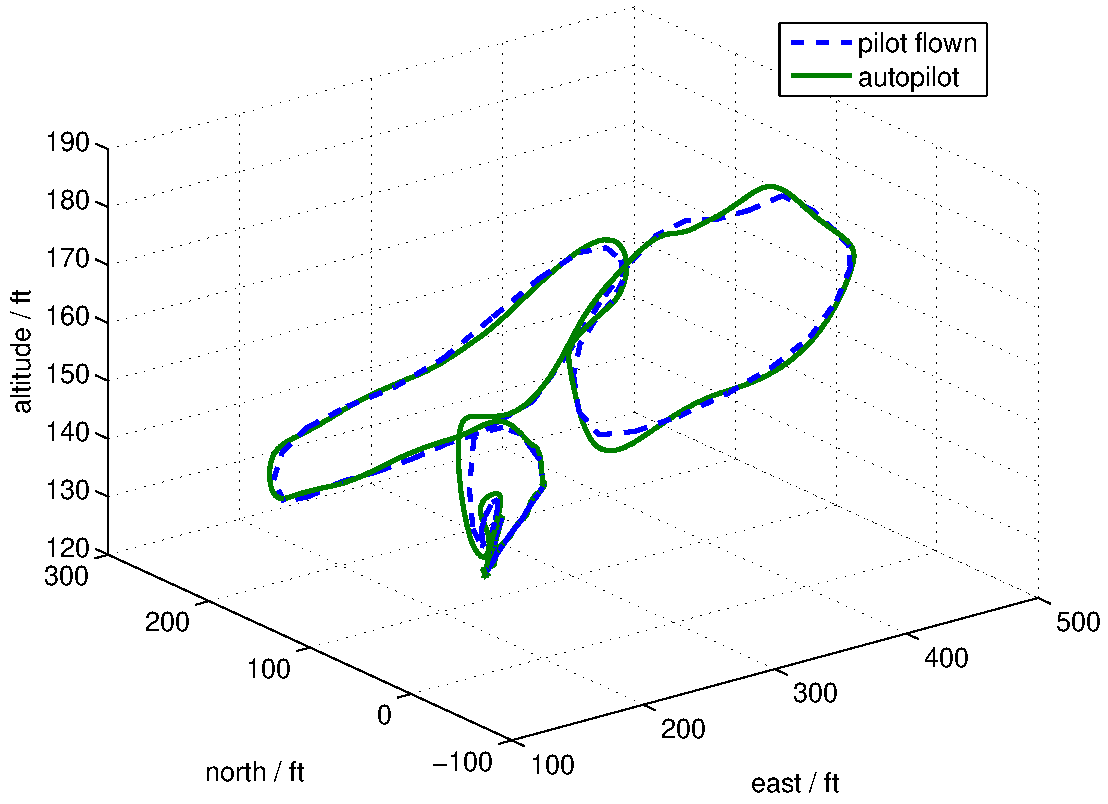
\includegraphics[height=\myfigheight]{pilottrack3d}
  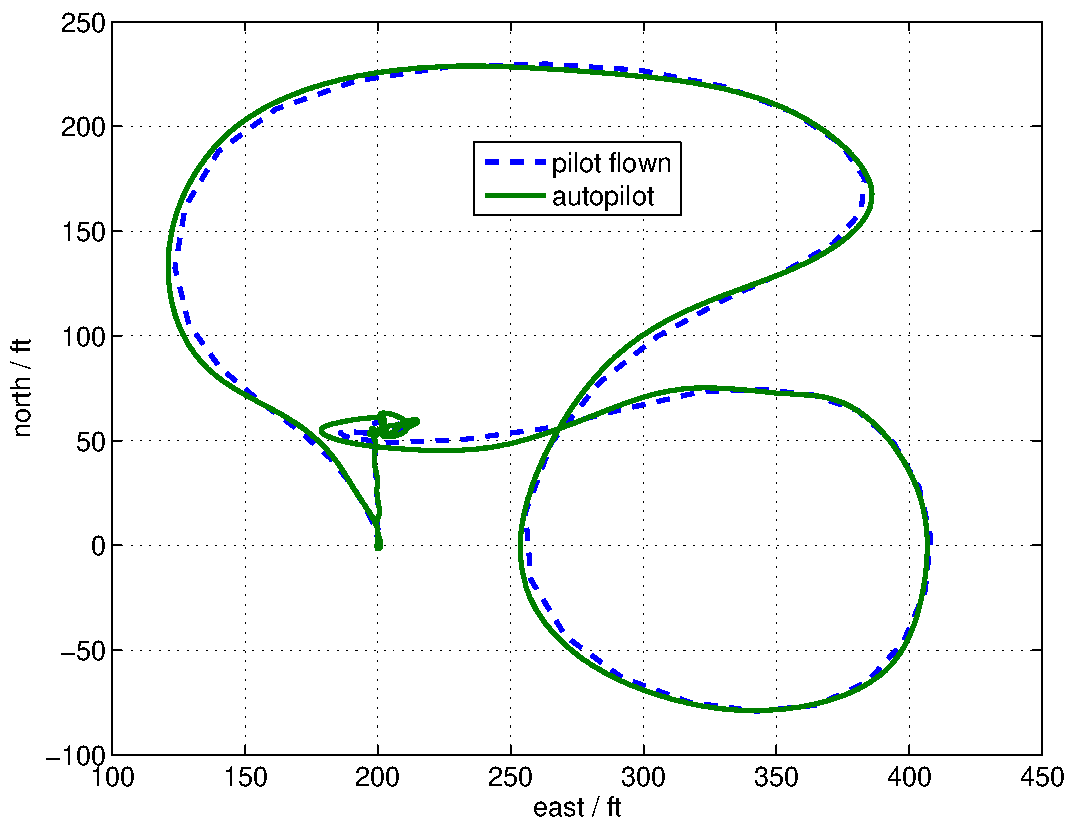
\includegraphics[height=\myfigheight]{pilottrackNorthEast}
  \caption{A 3D view and ground track view, of a trajectory initially flown manually by a pilot and then tracked by the controller.}
  \label{f:pilottrack3d}
  \end{center}
\end{figure}


Next, the ability of the controller to track a previous
manually-flown maneuver was tested. First, a human pilot flew a
figure eight, 3-dimensional pattern with the vehicle. Vehicle state
was recorded and was then played back as commands to the adaptive
controller. A 3D plot of the pilot and controller flown trajectories
are shown in \fig{f:pilottrack3d} along with projected ground track.
Overall, the tracking in position was measured to be within $11.3
ft$ of the desired pilot flown trajectory with a standard deviation
of $4.7 ft$.
%
%  \subfigure[\label{f:eturnNorthAltitude}]{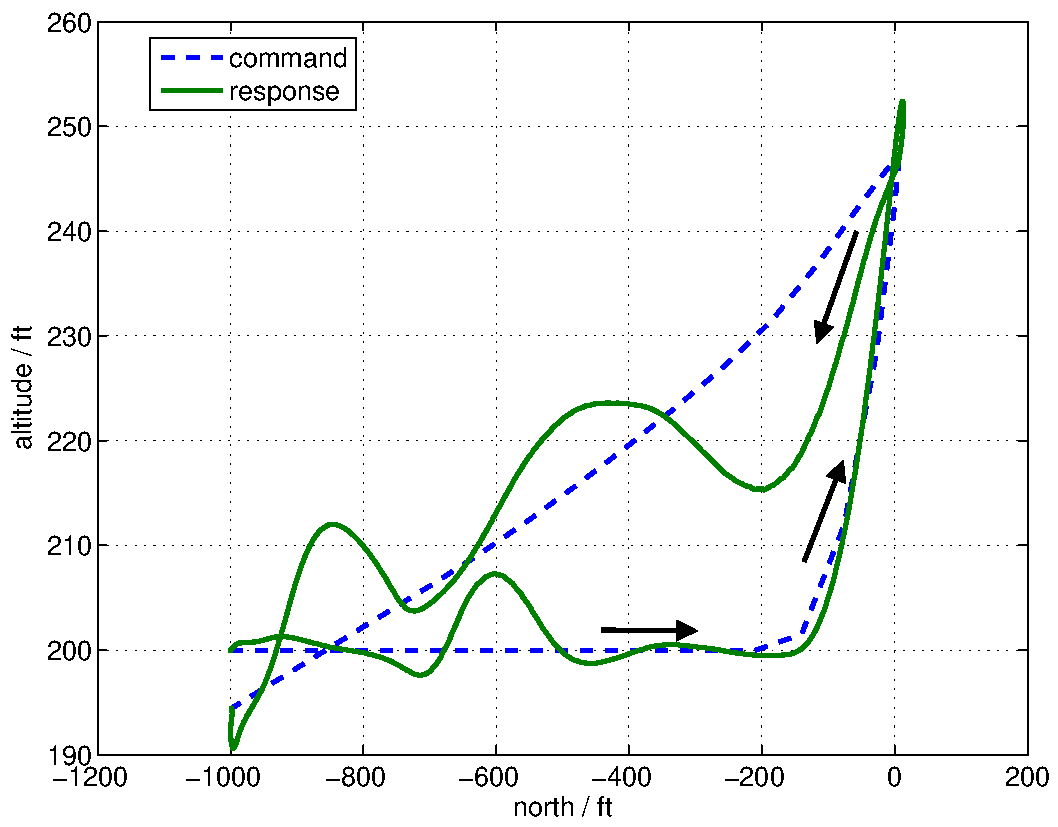
\includegraphics[height=\myfigheight]{eturnNorthAltitude}}
%  \subfigure[\label{f:eturnAlt}]{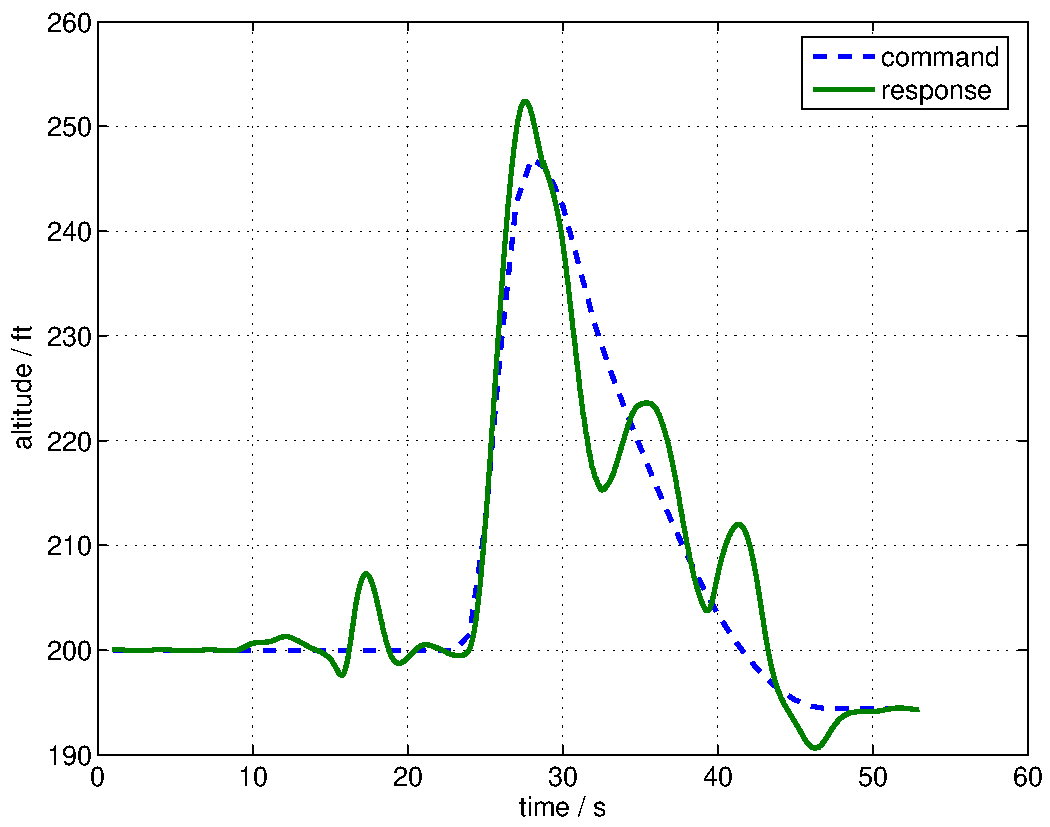
\includegraphics[height=\myfigheight]{eturnAlt}}
%  \subfigure[\label{f:eturnTheta}]{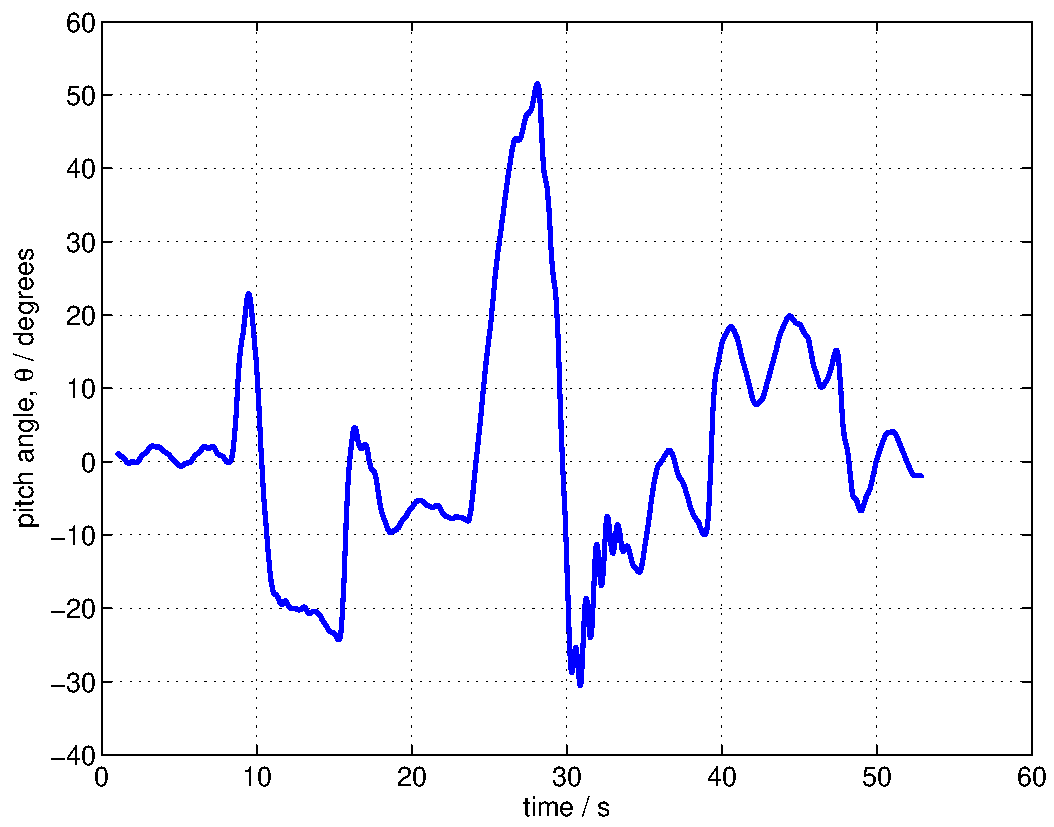
\includegraphics[height=\myfigheight]{eturnTheta}}
%  \subfigure[\label{f:eturnColl}]{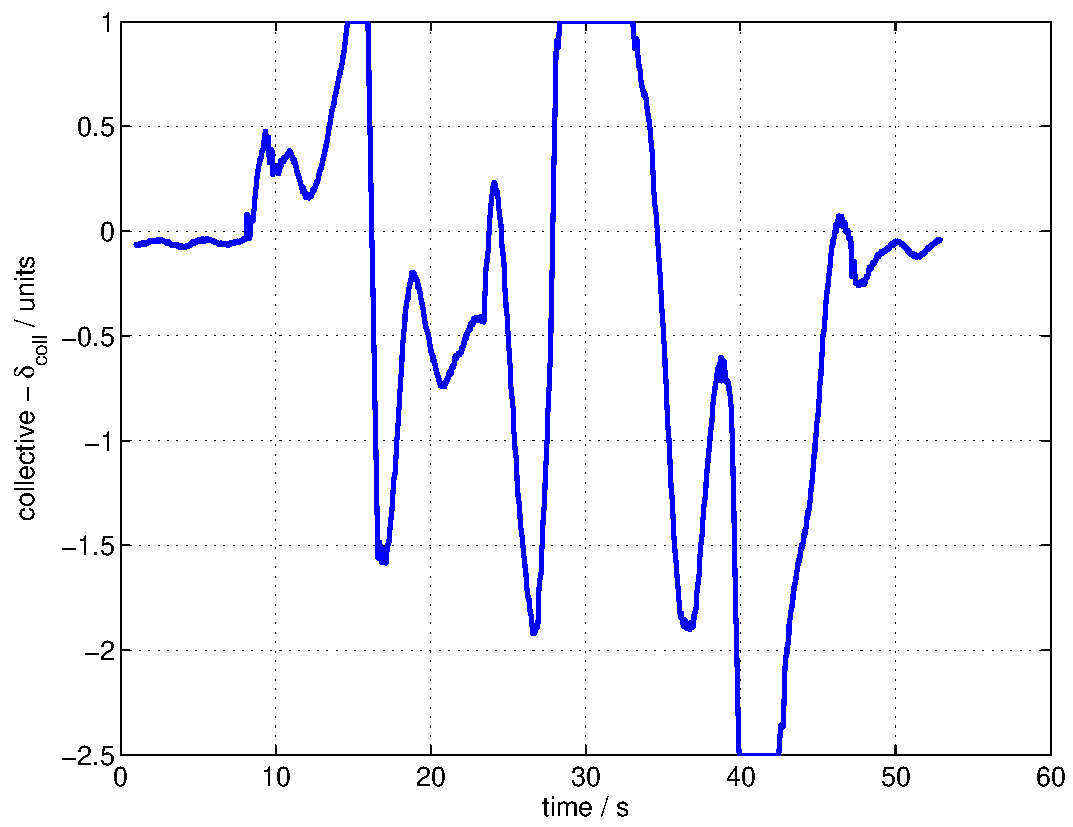
\includegraphics[height=\myfigheight]{eturnColl}}

\begin{figure}
  \begin{center}
  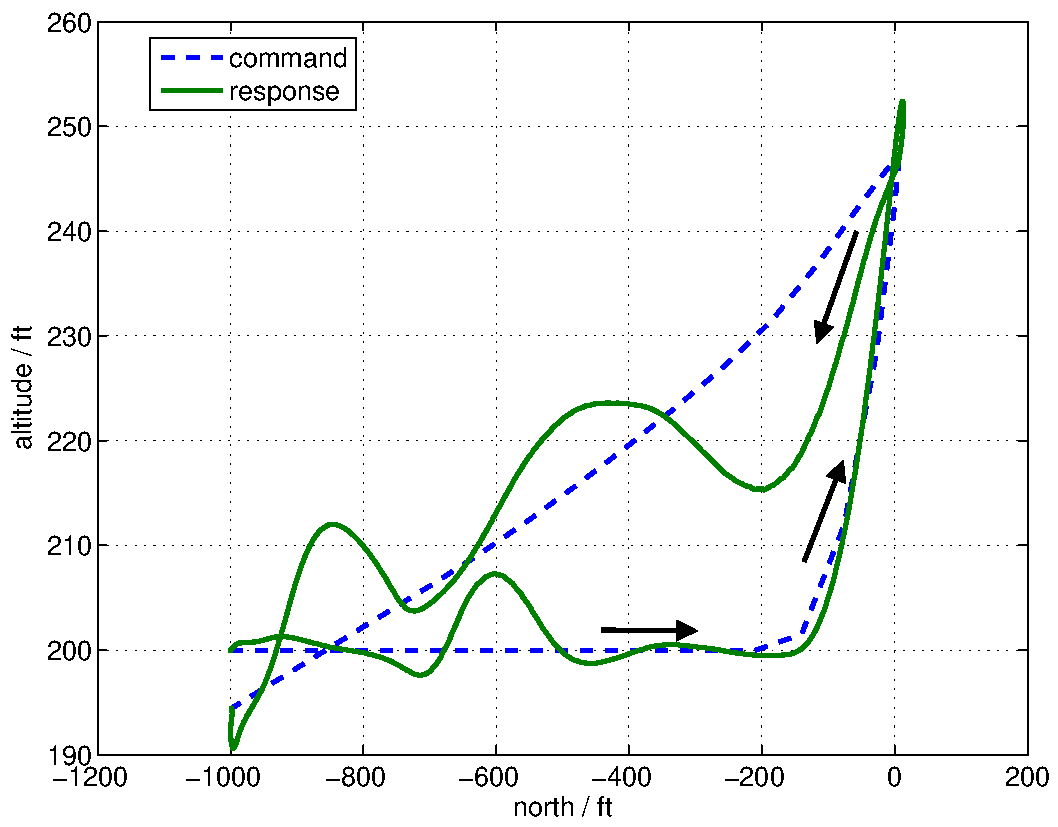
\includegraphics[height=\myfigheight]{eturnNorthAltitude}
  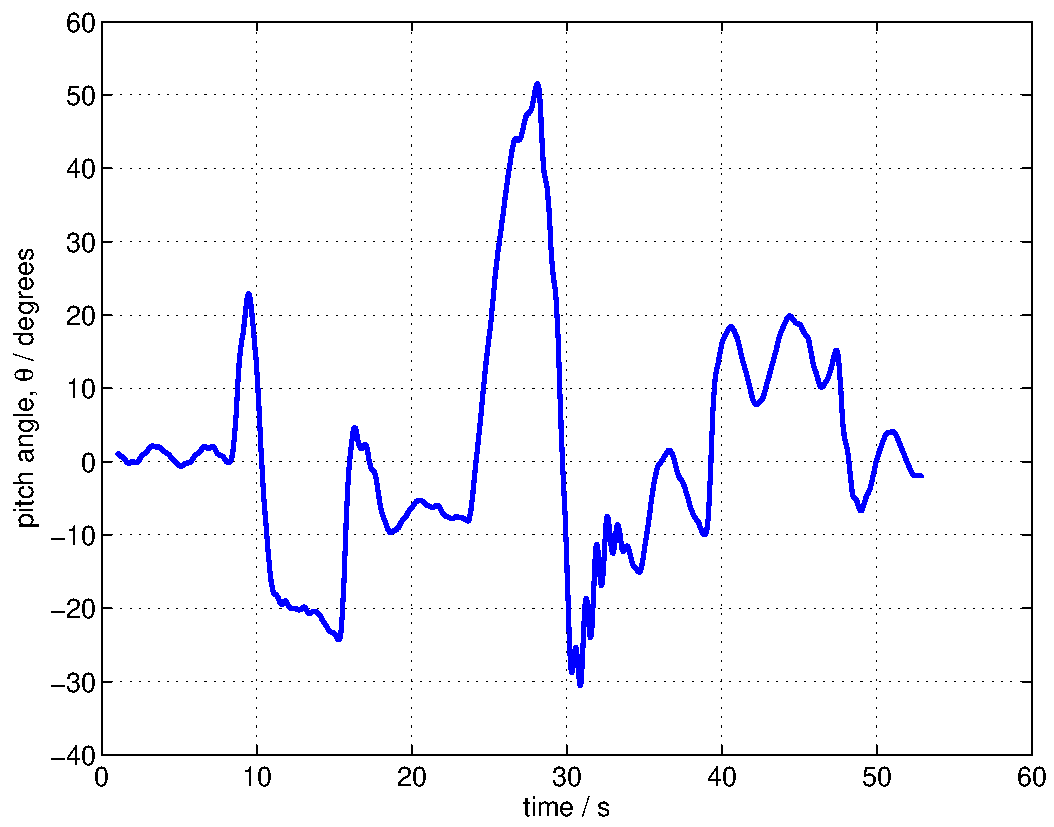
\includegraphics[height=\myfigheight]{eturnTheta}
  \caption{North-Altitude and pitch angle profile during a 180\textdegree\ velocity change maneuver. \emph{Note: North axis and Altitude axis scales are not equal}.}
  \label{f:eturnAltTheta}
  \end{center}
\end{figure}

\begin{figure}
  \begin{center}
  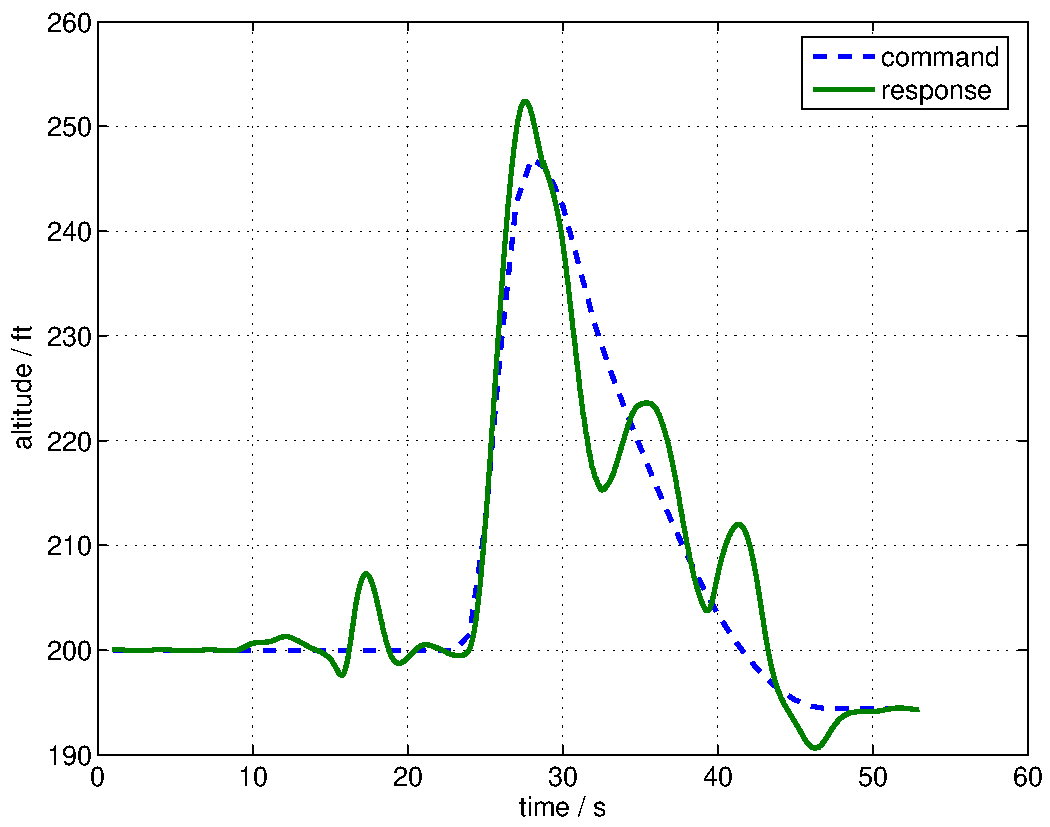
\includegraphics[height=\myfigheight]{eturnAlt}
  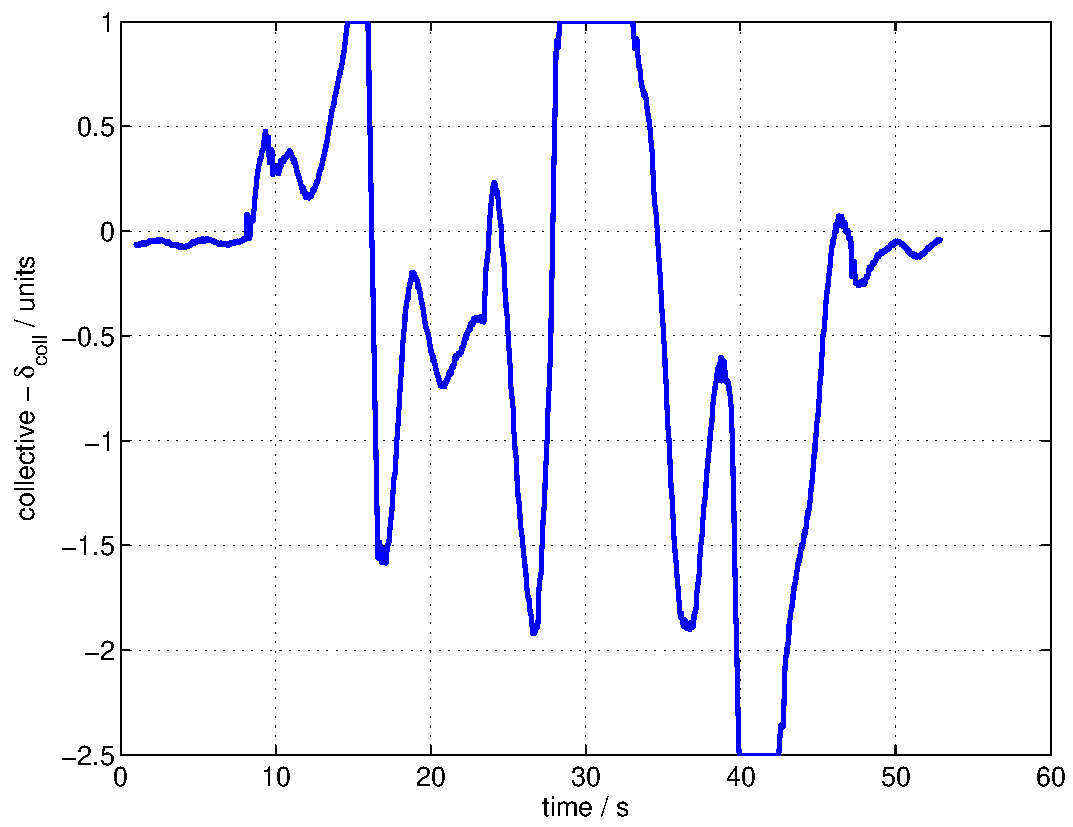
\includegraphics[height=\myfigheight]{eturnColl}
  \caption{Altitude and collective control history during a 180\textdegree\ velocity change maneuver.}
  \label{f:eturnAltColl}
  \end{center}
\end{figure}

Finally, a tactically useful maneuver was flown to test controller
performance at high speeds and pitch attitudes. The objective of the
maneuver is to make a 180-degree velocity change from a forward
flight condition of $70 ft/s$ north to a $70 ft/s$ forward flight
going south. The trajectory command and response in the
north-altitude plane is shown in \fig{f:eturnAltTheta} along with
the pitch angle. A time history of the altitude and the collective
control deflection is shown in \fig{f:eturnAltColl}. During the
maneuver the helicopter is commanded to increase altitude by up to
$50 ft$ in order to minimize saturation of the down collective. In
the deceleration phase the vehicle is able to track the command
trajectory well; however in accelerating to $70 ft/s$ going south,
tracking performance suffers. In both the acceleration and
deceleration phases, poor tracking corresponds with saturation of
the collective control. The oscillations in altitude in
\fig{f:eturnAltColl} are expected and are due to control saturation
which limits the vehicle's descent rate. The large pitch attitudes
experienced are what the outer-loop inversion evaluates as being
required to perform such rapid decelerations and accelerations. This
experiment is an example of maneuvering where the commanded
trajectory is more aggressive than the capability of the vehicle and
is reflected by the extended periods of saturation. It is possible
to operate at the limits of the vehicle primarily due to PCH which
protects the adaptation process.
%
%%%% pirouette
%
%\begin{figure}
%  \begin{center}
%  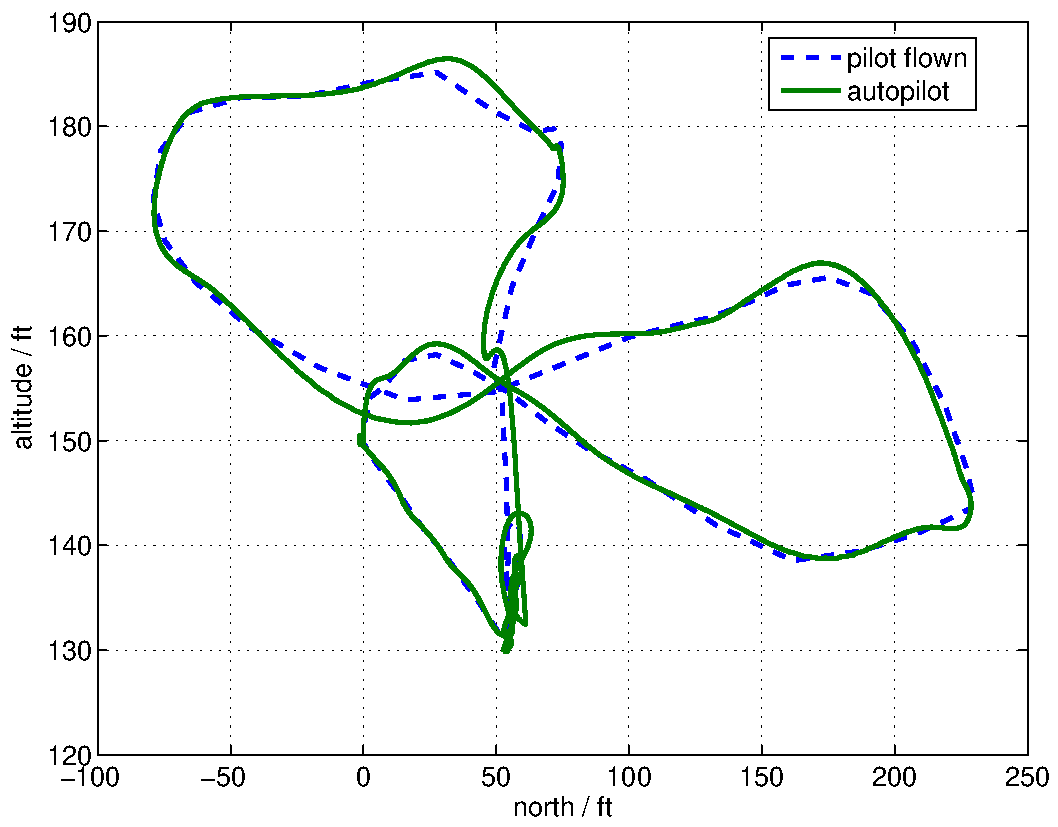
\includegraphics[height=\myfigheight]{pilottrackNorthAltitude}
%  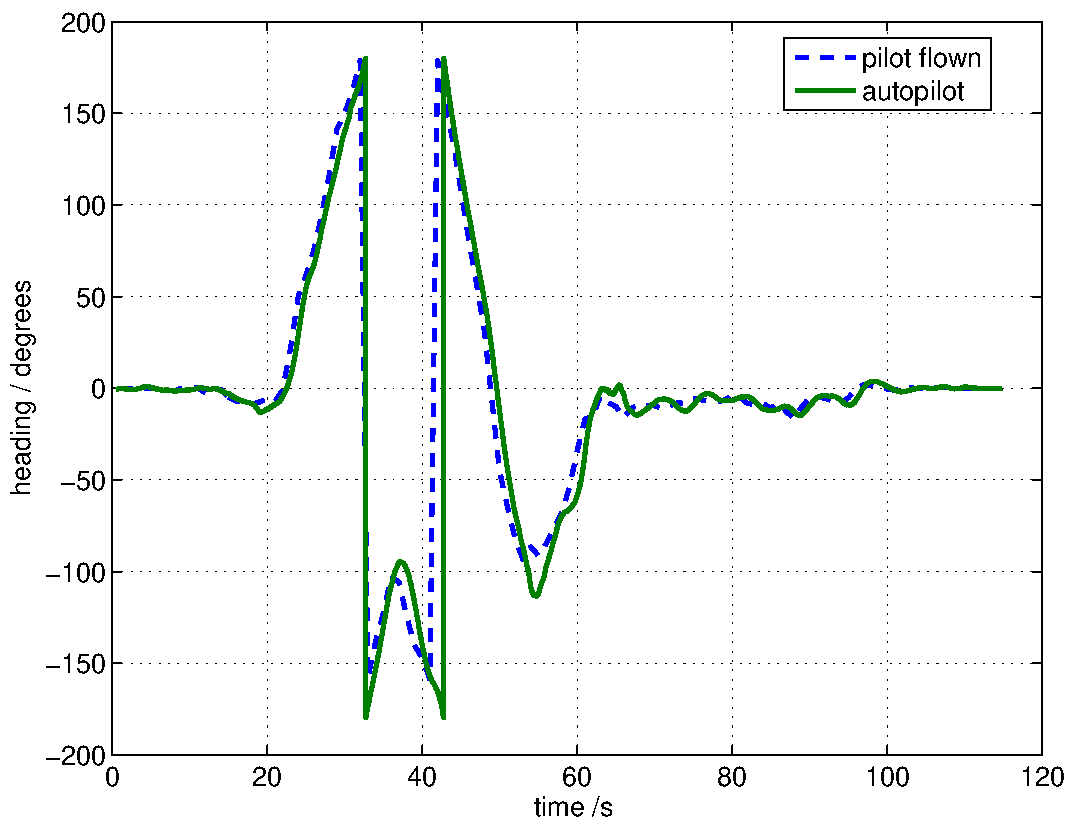
\includegraphics[height=\myfigheight]{pilottrackHeading}
%  \caption{North-Down plane and heading tracking of a trajectory initially flown manually by a pilot and then tracked by the controller.}
%  \label{f:pilottrackAltHead}
%  \end{center}
%\end{figure}
%
\subsection{Application to a Ducted Fan}
\begin{figure}
  \begin{center}
  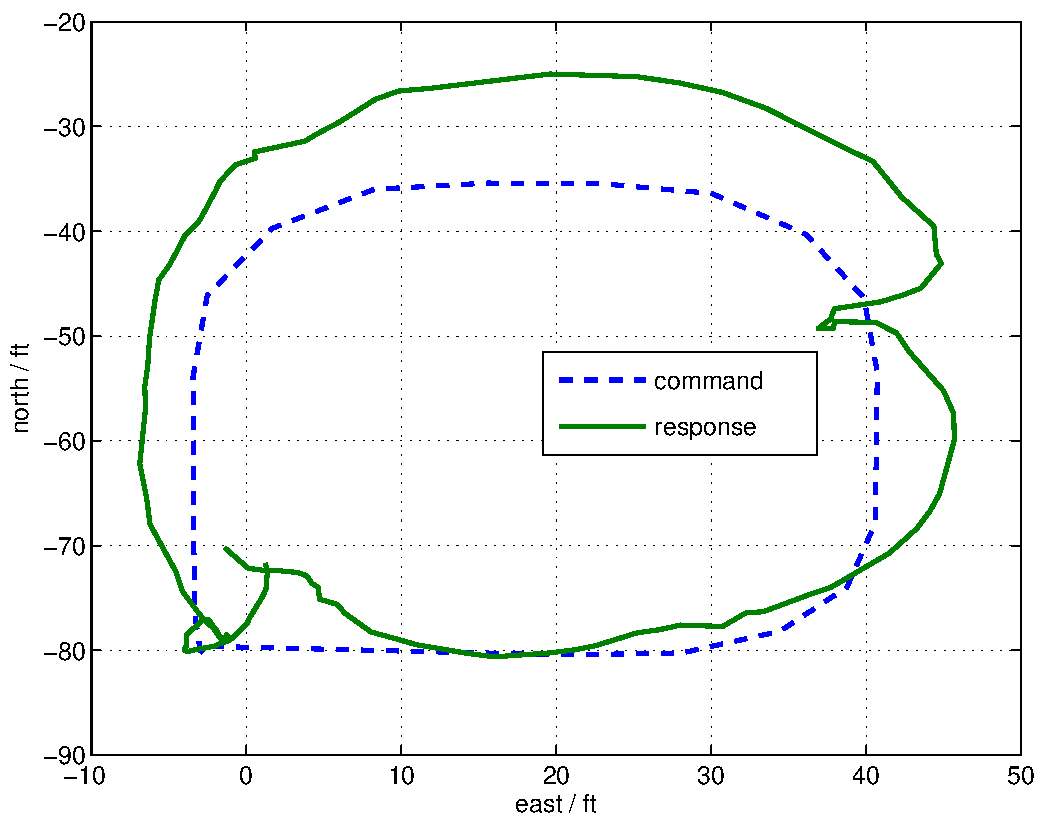
\includegraphics[height=\myfigheight]{gtspyBox2}
  \caption{The GTSpy performing a box maneuver}
  \label{f:gtspyBox}
  \end{center}
\end{figure}
%
\begin{figure}[h]
  \begin{center}
  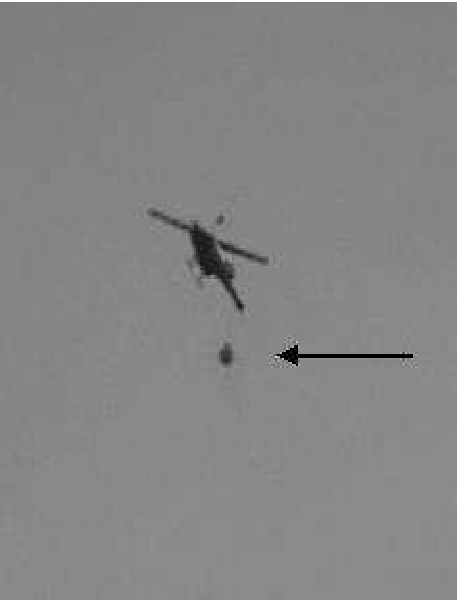
\includegraphics[height=\myfigheight]{gtspyMidAir}
  \caption{Deployment of the GTSpy ducted fan from the GTMax helicopter}
  \label{f:gtspyMidAir}
  \end{center}
\end{figure}
Following tests on the GTMax helicopter, the control method
presented in this chapter was applied to other smaller aircraft. The
algorithms were ported to a custom DSP/FPGA hardware device (the
FCS20) along with a small sensor board that contained gyroscopes and
accelerometers for inertial sensing and a GPS. The avionics package
weighed less than $1 lb$ and fell within the payload capacity of the
11-inch ducted fan (GTSpy). The GTSpy has a maximum take-off weight
of $5.5 lbs$ and is driven by a two-bladed fixed-pitch propeller.
The propeller is enclosed in an annular wing duct with an outer
diameter of $11 inches$. Vanes located directly beneath the
propeller move in order to provide yaw control about the propeller
axis. Two sets of control surfaces located further below the
propeller move in order to provide pitch and roll moments.
Maneuvering is accomplished by tilting the thrust vector with the
control surfaces relying primarily on inflow for dynamic pressure
during hover. Following satisfactory tethered tests, the vehicle was
untethered and allowed to fly simple missions. \fig{f:gtspyBox}
shows a plan view of a small $50\time50 ft$ box maneuver and the
GTSpy's tracking. The large deviation on the eastern side of the box
is most likely due to a wind gust. Another maneuver performed was
the mid-air deployment of the GTSpy. The GTSpy was mounted on the
GTMax helicopter with its engine on and then deployed from a safe
altitude. The GTSpy was able to recover from the initial deployment
transient and maintain attitude and position within 5 seconds of
launch. \fig{f:gtspyMidAir} shows the GTSpy and GTMax during the
deployment transient. Both the GTMax and GTSpy were under computer
control during this maneuver and is the first known deployment of a
rotorcraft from another rotorcraft.
%

%\processdelayedfloats
%
\subsection{Application to a Fixed Wing Aircraft}
The control method presented in this chapter was further applied to a
high-thrust-to-weight ratio fixed wing aircraft with conventional
aircraft controls and a fixed pitch two-bladed propeller. The
dynamic inverse used for control purposes approximated the aircraft
in hover mode where the body axis was defined as
\[
x_{heli} = L_2(-\pi/2)x_{airplane}
\]
where $L_2$ is a rotation matrix around the airplane's body y-axis.
Hence the ailerons control helicopter-yaw, the rudder controls
helicopter-roll and the elevators continue to control pitch. The
external commands provided to the control algorithm contains a
commanded pitch angle as a function of speed. Inner-loop gains were
based on $2.5, 1.5, 2.5 rad/s$ for the (helicopter) roll, pitch and
yaw axis respectively. Outer-loop gains were based on $1.5, 1.0, 0.7
rad/s$ for the x, y and z helicopter-body-axis respectively. The
output-layer learning rates $\Gamma_W$ was set to unity on all
channels and a learning rate of $\Gamma_V$ was set for all inputs.
Reference model parameters were set to $v_{lim} = 10 ft/s$ and
$\omega_{lim} = 1.0 rad/s$. The control effectiveness $B$ was scaled
based on speed in order to reflect the reduced control authority of
the control surfaces in hover. Flight tests were initiated with the
airplane performing circular orbits and gradually lowering airspeed
until hover. The reverse, transition to forward flight was
accomplished by a more aggressive command into forward flight.
\begin{figure}
  \begin{center}
  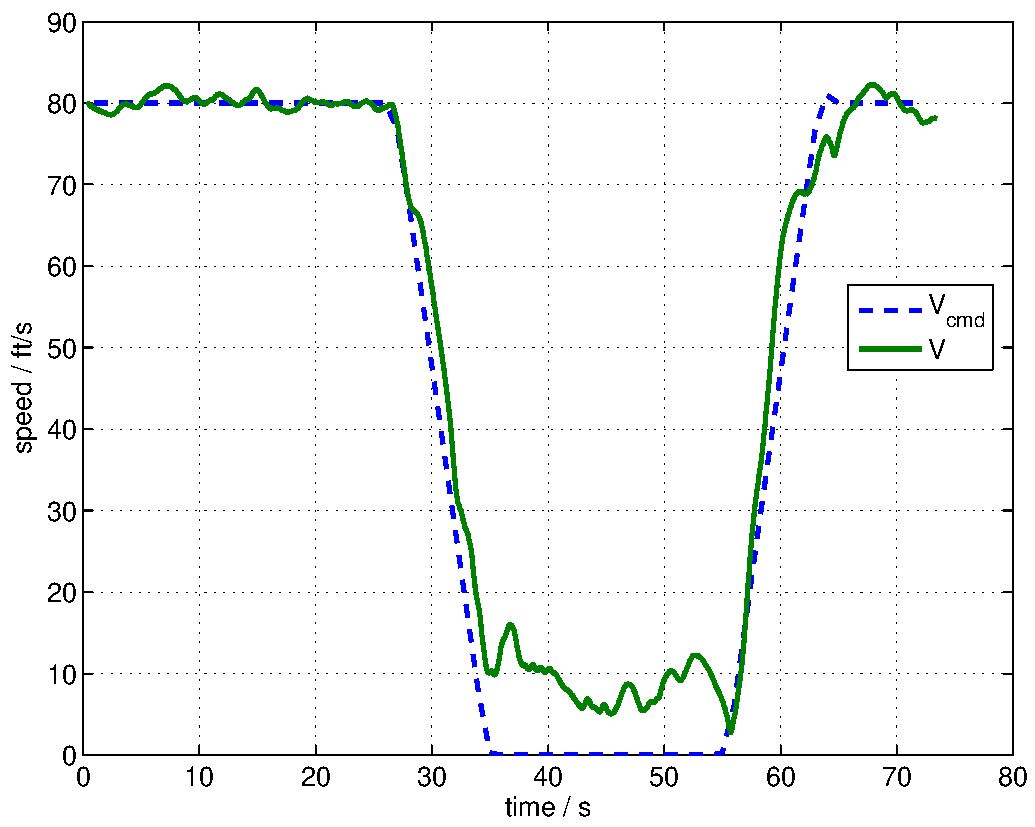
\includegraphics[height=\myfigheight]{edgeTransitionSpeed}
  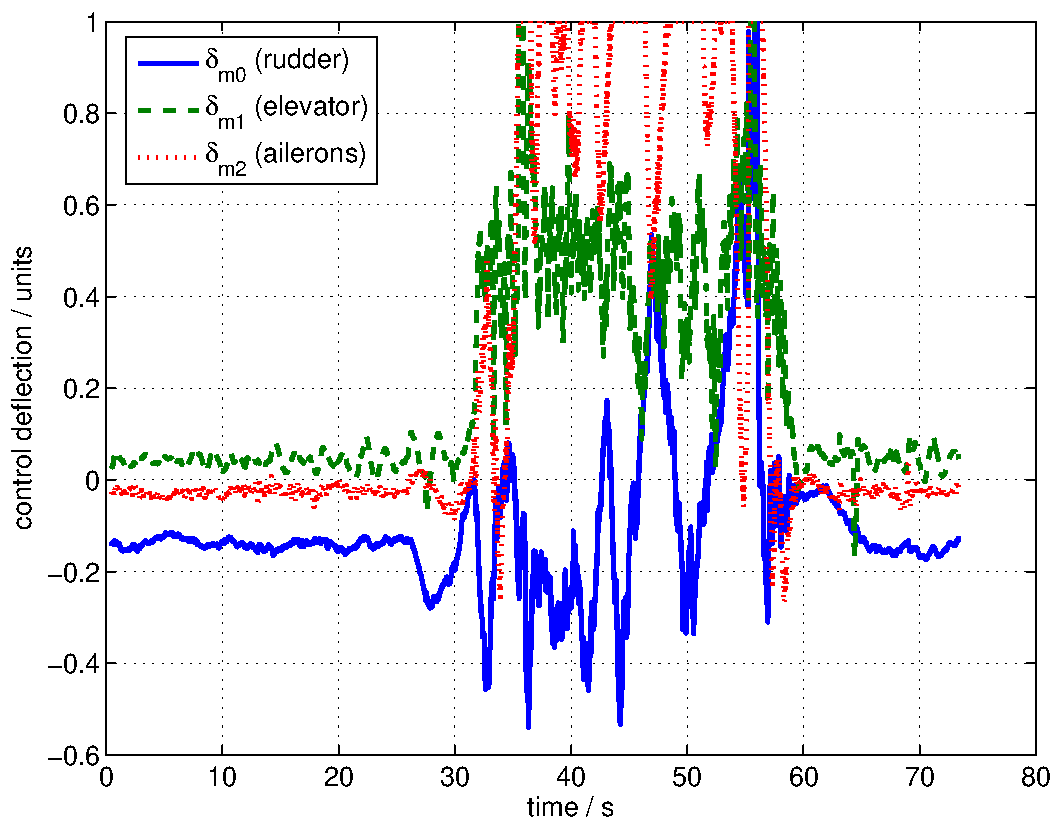
\includegraphics[height=\myfigheight]{edgeTransitionMomentControls}
  \caption{GTEdge speed profile and control deflections during transitions between hover and forward flight}
  \label{f:gtedgeSpeedMomentControls}
  \end{center}
\end{figure}

The following figures illustrate the response of the aircraft during
transitions between hover and forward flight.
\fig{f:gtedgeSpeedMomentControls} shows the vehicle in forward
flight at $80 ft/s$ performing a circular orbit. At $t = 26s$ a
transition to hover is initiated by supplying external trajectory
commands that lower the vehicle's speed. Transition is completed at
$t = 35 s$ with a low residual speed of approximately $5 ft/s$. At
$t = 55 s$ a transition back to forward flight at $80 ft/s$ is
initiated and completed at $t = 65 s$. During hover, $t\in[35,55]$,
the control deflections are seen to be significantly higher due to
the lower effectiveness at lower speeds. The ailerons are saturated
for significant intervals in a particular direction in order to
counteract engine torque.


\fig{f:gtedgePitchThrottle} illustrates the (helicopter) pitch angle
during transitions as well as the throttle control deflections. In
forward flight, the pitch angle is approximately $-75 deg$ and
varies in hover due to reduced control effectiveness and the
presence of a steady wind. Additionally, \fig{f:gtedgeTrajectory}
shows the position trajectory during transitions whereas
\fig{f:gtedgeDuringTransition} is a snapshot of the aircraft during
the maneuver.

\begin{figure}
  \begin{center}
  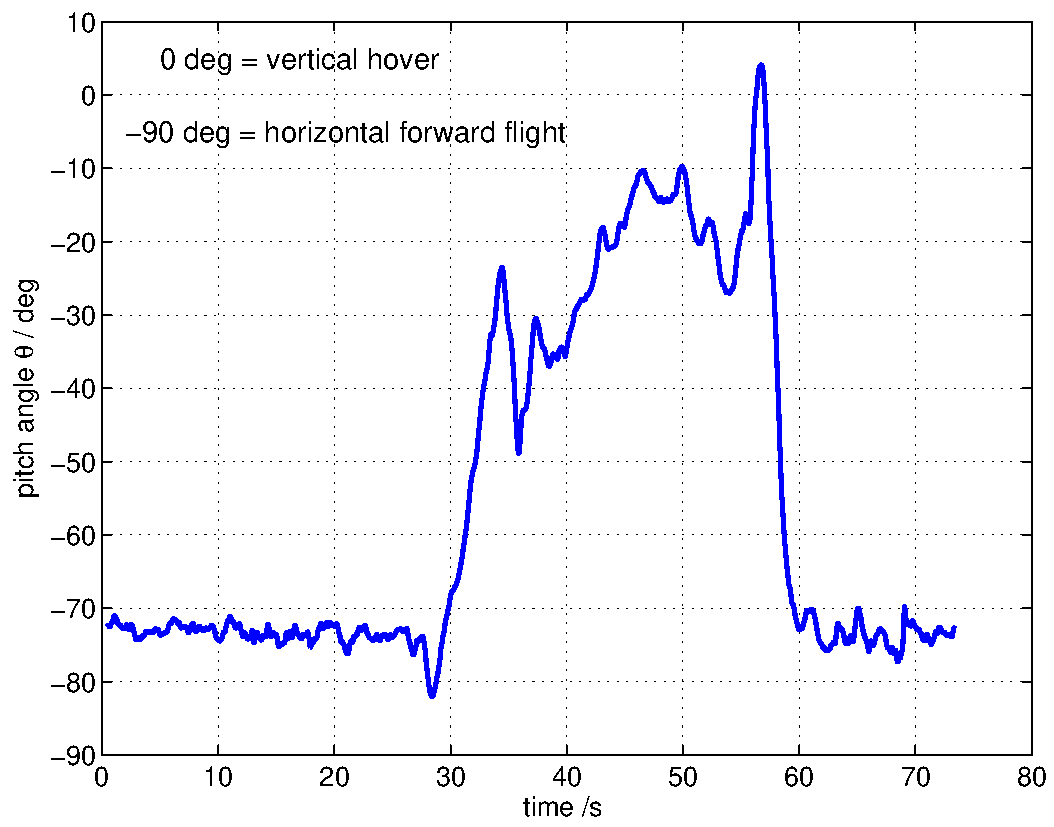
\includegraphics[height=\myfigheight]{edgeTransitionPitchAngle}
  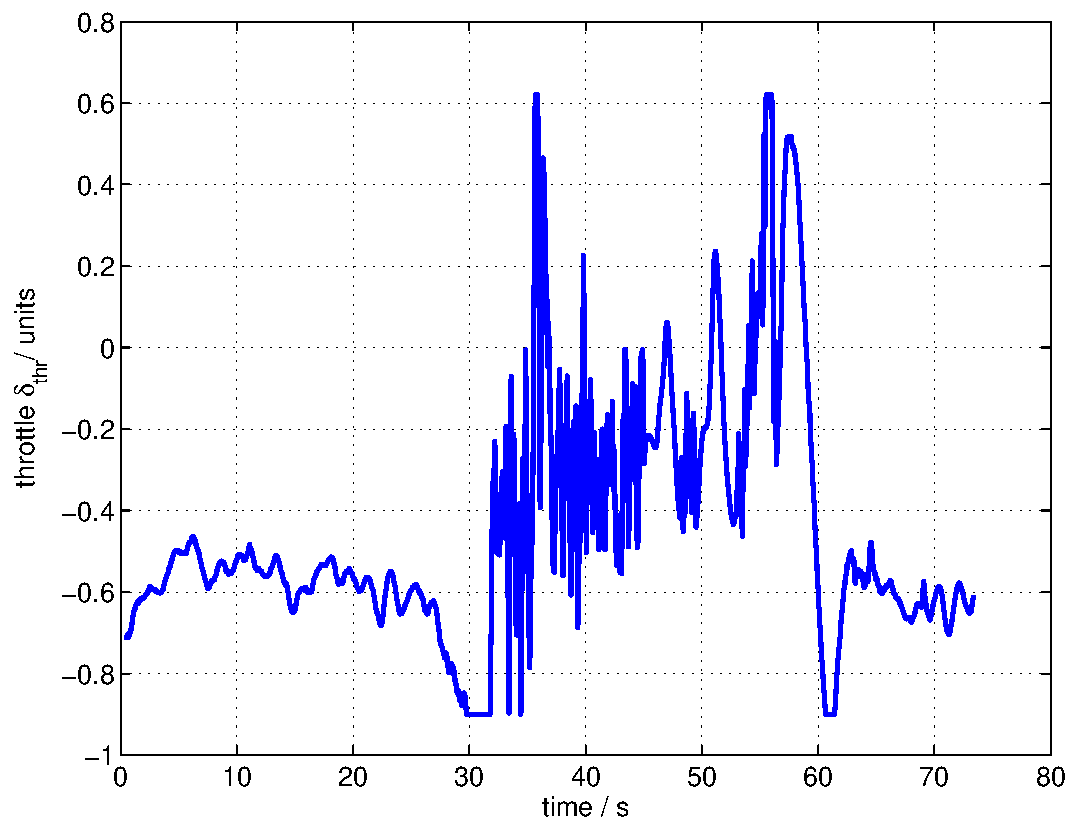
\includegraphics[height=\myfigheight]{edgeTransitionThrottle}
  \caption{GTEdge pitch angle, throttle profile during transitions between hover and forward flight}
  \label{f:gtedgePitchThrottle}
  \end{center}
\end{figure}

\begin{figure}
  \begin{center}
  \includegraphics[height=\myfigheight]{edgeTransitionNorthEastPlanView}
  \caption{GTEdge trajectory during transitions}
  \label{f:gtedgeTrajectory}
  \end{center}
\end{figure}

\begin{figure}
  \begin{center}
  \includegraphics[height=\myfigheight]{edgeDuringTransition}
  \caption{GTEdge during a transition}
  \label{f:gtedgeDuringTransition}
  \end{center}
\end{figure}

\todo{Shorten the subsection titles and perhaps  make subusb section into a subsection}
\subsection{Implementation of Concurrent Learning Adaptive Controller on a VTOL UAV}\label{s:conc_flight_test}
\todo[inline,color=green]{Some of this section is redundant, we should refer back to previous descriptions of the experimental setup, or simply not mention it because it will just flow}
\todo[inline]{A little smoothing will fix disconnect}
Flight-test results of the concurrent learning adaptive law described in Section \ref{s:conc} are presented in this section. The test vehicle is the GTMax rotorcraft UAV. The modification to the adaptive controller described in Section \ref{s:controller} include the concurrent learning adaptive law of Equations \ref{eq:bg_learninglaw} for a nonlinearly parameterized SHL NN. Data points were selected online based on Equation \ref{eq:points_criterion} and were stored in a history stack limited to carrying $20$ points. Once the history stack was full,  a new data point was added by replacing the oldest data point. A fixed point smoother was used to estimate $\dot x_j$ for a recorded data point using both forward and a backward Kalman filter \cite{Chowdhary:JGCD:10,Gelb:74bk}. Typically this induced a selectable time-delay introduced by the time required for the smoother to converge, however, this does not affect the instantaneous tracking error.

\subsubsection{Repeated Forward Step Maneuvers}
\label{sec:bg_steps}
The repeated forward step maneuvers are chosen in order to create a relatively simple situation in which the controller performance can be compared over several similar maneunvers. By using concurrent learning NN improved performance is expected through repeated maneuvers and a faster convergence of weights. Figure \ref{fig:steps_all_states}  shows the body frame states from recorded flight data for a chain of forward step inputs. Figure \ref{fig:steps_errors_il_bg} and Figure \ref{fig:steps_errors_ol_bg} shows the evolution of inner and outer loop errors. These results assert the stability (in the ultimate boundedness sense) of the combined concurrent and online learning approach.

Figure \ref{fig:steps_W_bg} and Figure \ref{fig:steps_V_bg} show the evolution of NN $W$ and $V$ weights as the rotorcraft performs repeated step maneuvers and the NN is trained using the concurrent learning method of Theorem \ref{th:bg_bounded}. The NN $V$ weights (\ref{fig:steps_V_bg}) appear to go to constant values when concurrent learning adaptation is used, this can be contrasted with Figure \ref{fig:steps_V_o} which shows the $V$ weight adaptation for a similar maneuver without concurrent learning. NN $W$ weights for both cases remain bounded, however it is seen that with concurrent learning adaptation the NN $W$ weights seem to separate, this indicates alleviation of the rank-1 condition experienced by the baseline adaptive law relying only on instantaneous data \cite{Chowdhary:JGCD:10}. The flight test results indicate a noticeable improvement in the error profile. In Figure \ref{fig:steps_all_states} it is seen that the UAV tends not to have a smaller component of body lateral velocity ($v$) through each successive step. This is also seen in Figure \ref{fig:steps_errors_ol_bg}  where it is noted that the error in $v$ (body $y$ axis velocity) reduces through successive steps.  These effects in combination indicate that the combined online and concurrent learning system is able to improve performance over the baseline controller through repeated maneuvers, indicating long term learning.  These results are of particular interest, since the maneuvers performed were conservative, and the baseline adaptive MRAC controller had already been extensively tuned.



\begin{figure}[h]
\centering
\includegraphics[scale=0.5]{steps_all_states}
\caption{Recorded Body Frame States for Repeated Forward Steps}
\label{fig:steps_all_states}
\end{figure}

\begin{figure}[h]
\centering
\subfigure[Evolution of inner loop errors with concurrent Adaptation]{\label{fig:steps_errors_il_bg}\includegraphics[scale=0.5]{steps_bg_il_errors}}
\subfigure[Evolution of outer loop errors with concurrent Adaptation]{\label{fig:steps_errors_ol_bg}\includegraphics[scale=0.5]{steps_bg_ol_errors}}
\caption{GTMax Recorded Tracking Errors for Successive Forward Step Inputs with concurrent Learning}
\label{fig:steps_errors}
\end{figure}


\begin{figure}[h]
\centering
\subfigure[Evolution of $V$ matrix weights with Only Online Adaptation]{\label{fig:steps_V_o}\includegraphics[scale=0.5]{sim_online_v}}
\subfigure[Evolution of $V$ matrix weights with concurrent Adaptation]{\label{fig:steps_V_bg}\includegraphics[scale=0.5]{steps_bg_V}}
\subfigure[Evolution of $W$ matrix weights with Only Online Adaptation]{\label{fig:steps_W_o}\includegraphics[scale=0.5]{sim_online_w}}
\subfigure[Evolution of $W$ matrix weights with concurrent Adaptation]{\label{fig:steps_W_bg}\includegraphics[scale=0.5]{steps_bg_W}}
\caption{Comparison of Weight Convergence on GTMax with and without concurrent Learning}
\label{fig:steps_weights}
\end{figure}
%%
\subsubsection{Aggressive Trajectory Tracking Maneuvers}
Flight-test results are presented for concurrent learning adaptive controllers while tracking repeatedly an elliptical trajectory with aggressive velocity ($50 ft/s$) and acceleration ($~20 ft/s^2$) profile. Since these maneuvers involve state commands in more than one system state it is harder to visually inspect the data and see whether an improvement in performance is seen, therefore the Euclidian norm of the error signal at each time step is used as a rudimentary metric. Figure \ref{fig:all_states_agg_ovals} shows the recorded inner and outer loop states as the rotorcraft repeatedly tracks an oval trajectory pattern. In this flight, the first two ovals (until t = 5415 s) are tracked with a commanded acceleration of $30ft/sec^2$, while the rest of the ovals are tracked at $20ft/sec^2$. In the following both these parts of the flight test are discussed separately.

\subsubsection{Aggressive Trajectory Tracking with Saturation in the Collective Channel}
\label{sec:bg_oval}
Due to the aggressive acceleration profile of $30ft/s^2$ the rotorcraft collective channels were observed to saturate while performing high velocity turns. This leads to an interesting challenge for the adaptive controller equipped with pseudo-control hedging. Figure \ref{fig:oval_sat_errors} shows the evolution of the innerloop and outerloop tracking error. It can be clearly seen that the tracking error in the $u$ (body x axis velocity) channel reduces in the second pass through the ellipse indicating long term learning by the combined online and concurrent learning adaptive control system. This result is further characterized by the noticeable reduction in the norm of the tracking error at every time step as shown in Figure \ref{fig:bg_agg_Sat_error_norm} \todo{this should reference something 24 is hardcoded}.



\begin{figure}[h]
\centering
\includegraphics[scale=0.6]{all_states_agg_oval}
\caption{Recorded Body Frame States for Repeated Oval Maneuvers}
\label{fig:all_states_agg_ovals}
\end{figure}

\begin{figure}[h]
\centering
\subfigure[Evolution of inner loop errors with concurrent Adaptation]{\label{fig:bg_agg_sat_il_e}\includegraphics[scale=0.5]{bg_agg_sat_il_e}}
\subfigure[Evolution of outer loop errors with concurrent Adaptation]{\label{fig:bg_agg_sat_ol_e}\includegraphics[scale=0.5]{bg_agg_sat_ol_e}}
\caption{GTMax Recorded Tracking Errors for Aggressive Maneuvers with Saturation in Collective Channels with concurrent Learning}
\label{fig:oval_sat_errors}
\end{figure}

\begin{figure}[h]
\centering
\includegraphics[scale=0.7]{bg_agg_sat_error_norm}
\caption{Plot of the norm of the error at each time step for aggressive trajectory tracking with collective saturation}
\label{fig:bg_agg_Sat_error_norm}
\end{figure}

\subsubsection{Aggressive Trajectory Tracking Maneuver}
For the results presented in this section, the acceleration profile was reduced to $20ft/sec^2$. At this acceleration profile, no saturation in the collective input was noted. Figure \ref{fig:oval_nosat_errors} shows the evolution of tracking error, and Figure \ref{fig:bg_agg_nosat_error_norm} shows the plot of the norm of the tracking error at each time step.
\begin{figure}[h]
\centering
\subfigure[Evolution of inner loop errors with concurrent Adaptation]{\label{fig:bg_agg_nosat_il_e}\includegraphics[scale=0.5]{bg_agg_nosat_il_e}}
\subfigure[Evolution of outer loop errors with concurrent Adaptation]{\label{fig:bg_agg_nosat_ol_e}\includegraphics[scale=0.5]{bg_agg_nosat_ol_e}}
\caption{GTMax Recorded Tracking Errors for Aggressive Maneuvers with concurrent Learning}
\label{fig:oval_nosat_errors}
\end{figure}

\begin{figure}[h]
\centering
\subfigure[Evolution of the norm of the tracking error with concurrent Adaptation]{\label{fig:bg_agg_nosat_error_norm}\includegraphics[scale=0.42]{bg_agg_nosat_error_norm}}
\subfigure[Evolution of the norm of the tracking error with only online Adaptation]{\label{fig:o_agg_nosat_error_norm}\includegraphics[scale=0.5]{online_agg_nosat_error_norm}}
\caption{Comparison of norm of GTMax Recorded Tracking Errors for Aggressive Maneuvers}
\label{fig:oval_comparision_error_norm}
\end{figure}

\subsubsection{Aggressive Trajectory Tracking Maneuvers with Only Online Learning NN}
The performance of the concurrent learning adaptive controller is compared with the traditional instantaneous update based adaptive controllers for the maneuvers described in Section \ref{sec:bg_oval}.

It is instructive to compare Figure \ref{fig:oval_V_bg}, and Figure \ref{fig:oval_W_bg} which show the evolution of the NN weights with only instantaneous learning with Figure \ref{fig:oval_V_o}, and Figure \ref{fig:oval_W_o} which show evolution of the NN weights with concurrent learning. Although absolute convergence of weights is not seen, as expected due to Theorem \ref{th:bg_bounded} it is interesting to see that when concurrent learning is on, the weights tend to be less oscillatory than when only instantaneous learning is used. Also, with combined online and concurrent learning, the weights do not tend to go to zero as the rotorcraft hovers between two successive tracking maneuver. Figure \ref{fig:o_agg_nosat_error_norm} shows the plot of the tracking error norm as a function of time without concurrent learning. Comparing this figure with Figure \ref{fig:bg_agg_nosat_error_norm} it can be clearly seen that the norm of the error vector is much higher when only online learning is used. This indicates that the combined online and concurrent learning adaptive controller has improved trajectory tracking performance.
\begin{figure}[h]
\centering
\subfigure[Evolution of $V$ matrix weights with Only Online Adaptation]{\label{fig:oval_V_o}\includegraphics[scale=0.5]{online_agg_nosat_V}}
\subfigure[Evolution of $V$ matrix weights with concurrent Adaptation]{\label{fig:oval_V_bg}\includegraphics[scale=0.5]{bg_agg_nosat_V}}
\subfigure[Evolution of $W$ matrix weights with Only Online Adaptation]{\label{fig:oval_W_o}\includegraphics[scale=0.5]{online_agg_nosat_W}}
\subfigure[Evolution of $W$ matrix weights with concurrent Adaptation]{\label{fig:oval_W_bg}\includegraphics[scale=0.5]{bg_agg_nosat_W}}
\caption{Comparison of Weight Convergence as GTMax tracks aggressive trajectory with and without concurrent Learning }
\label{fig:oval_weights}
\end{figure}
In summary, the flight test results ascertain an expected improvement in tracking performance.  Furthermore, the evolution of the neural network W and V matrix weights were observed to have different characteristics when concurrent learning was employed, including, weight separation, a tendency towards weight convergence in some cases, and different numerical values of the adaptive weights. This difference in neural network weight behavior demonstrates the effect of overcoming the rank-1 condition.



\section{Summary}
The objective in this chapter has been to provide an affordable control design solution that uses minimal prior knowledge of the vehicle dynamics. This is accomplished by relying on adaptation to cover the flight envelope of the helicopter under nominal conditions. Under mission specific variations in the environment and system dynamics due to payload changes or damage, adaptation allows little or no human intervention after deployment. This approach is also in agreement with the DoD UAS Roadmap which subscribes to the following view on UAV's \emph{...affordability will be treated as a key performance parameter (KPP) equal to, if not more important than, schedule and technical performance...}.

\appendix
\section{Adaptive Element}
\label{s:network}
Single hidden layer (SHL) perceptron NNs are
universal approximators\cite{hornik_89,spooner,lewis:ajc:99}. Hence,
given a sufficient number of hidden layer neurons and appropriate
inputs, it is possible to train the network online to cancel model
error.
%
\begin{figure}[h]
  \centering\includegraphics[width=.7\columnwidth]{nn}
%  \centering\includegraphics{nn}
  \caption{Neural Network with one hidden layer.}
  \label{f:nn}
\end{figure}
%
\fig{f:nn} shows the structure of a generic single hidden layer
network whose input-output map may be expressed as
\begin{equation}
\nu_{ad_k} = b_w\theta_{w_k} + \sum_{j=1}^{n_2}w_{jk}\sigma_j(z_j),
\end{equation}
where, $k=1,...,n_3$, $b_w$ is the outer layer bias,
$\theta_{w_k}$ is the $k^{th}$ threshold. $w_{jk}$ represents the
outer layer weights, $z_j$ is the input to the neurons, and the scalar $\sigma_j$ is a sigmoidal
activation function
\begin{equation}
\label{e:activation} \sigma_j(z_j) = \frac{1}{1 + e^{-az_j}},
\end{equation}
where, $a$ is the so called \emph{activation potential} and may
have a distinct value for each neuron. $z_j$ is the input to the
$j^{th}$ hidden layer neuron, and is given by
\begin{equation}
z_j = b_v\theta_{v_j} + \sum_{i=1}^{n_1}v_{ij}x_{in_i},
\end{equation}
where, $b_v$ is the inner layer bias and $\theta_{v_j}$ is the
$j^{th}$ threshold. Here, $n_1,n_2$ and $n_3$ are the number of
inputs, hidden layer neurons and outputs respectively. $x_{in_i},
i=1,...,n_1$, denotes the inputs to the NN. For convenience, define
the following weight matrices:
\begin{align}
V &\triangleq
\begin{bmatrix}
\theta_{v,1}    &     \cdots   & \theta_{v,n_2} \\
v_{1,1}         &     \cdots   & v_{1,n_2} \\
\vdots          &     \ddots   & \vdots \\
v_{n_1,1}       &     \cdots   & v_{n_1,n_2}
\end{bmatrix},  \\
W &\triangleq
\begin{bmatrix}
\theta_{w,1}    &     \cdots   & \theta_{w,n_3} \\
w_{1,1}         &     \cdots   & w_{1,n_3} \\
\vdots          &     \ddots   & \vdots \\
w_{n_2,1}       &     \cdots   & w_{n_2,n_3}
\end{bmatrix},  \\
\label{e:Z} Z &\triangleq
\begin{bmatrix}
V   &   0  \\
0   &   W
\end{bmatrix}.
\end{align}
%
Additionally, define the $\bfsigma(\bfz)$ vector as
\begin{equation}
\bfsigma^T(\bfz) \triangleq
\begin{bmatrix}
b_w    &    \sigma(z_1)  &  \cdots &  \sigma(z_{n_2}),
\end{bmatrix}
\end{equation}
where $b_w > 0$ allows for the thresholds, $\bftheta_w$, to be
included in the weight matrix $W$. Also, $\bfz = V^T\bar{\bfx}$,
where,
\begin{equation}
\bar{\bfx}^T =
\begin{bmatrix} b_v   & \bfx_{in}^T
\end{bmatrix},
\end{equation}
where, $b_v > 0$, is an input bias that allows for thresholds
$\bftheta_v$ to be included in the weight matrix $V$.
%
The input-output map of the SHL network may now be written in
concise form as
\begin{equation}
\label{e:nuad} \nuad = W^T\bfsigma(V^T\xbar).
\end{equation}
%
The NN may be used to approximate a nonlinear function, such as
$\Del(.)$. The universal approximation property\cite{hornik_89} of
NN's ensures that given an $\bar{\epsilon} > 0$, then $\forall$
$\xbar \in \domd$, where $\domd$ is a compact set, $\exists$ an
$\bar{n}_2$ and an ideal set of weights $(V^*,W^*)$, that brings the
output of the NN to within an $\epsilon$-neighborhood of the
function approximation error. This $\epsilon$ is bounded by
$\bar{\epsilon}$ which is defined by
\begin{equation}
\bar{\epsilon} = \sup_{\xbar \in \domd} \left\|
W^T\bfsigma(V^T\xbar) - \Del(\xbar) \right\|.
\end{equation}
The weights, $(V^*,W^*)$ may be viewed as optimal values of $(V,W)$
in the sense that they minimize $\bar{\epsilon}$ on $\domd$. These
values are not necessarily unique. The universal approximation
property thus implies that if the NN inputs $\bfx_{in}$ are chosen
to reflect the functional dependency of $\Del(\cdot)$, then
$\bar{\epsilon}$ may be made arbitrarily small given a sufficient
number of hidden layer neurons, $n_2$.

\begin{comment}
\subsubsection{Instantaneous update laws}
 Define $r=e^TPB$, where $P$ is the positive definite solution to the Lyapunov equation as defined in \ref{eq:Lyap}
    \begin{eqnarray}
    \label{eq:backprop_shl}
    \dot{W}=-(\sigma(\bar x)-\sigma'(V^T\bar{x})V^T\bar{x}) r^T \Gamma_W,\\
    \label{eq:backprop_shl_V}
    \dot{V} =  - \Gamma _V \bar xr^TW^T \sigma'(V^T\bar{x}),
    \end{eqnarray}
    where $\Gamma_W,\Gamma_V$ are positive definite matrices that define the learning rate of the NN. This update law closely resembles the backpropagation method of tuning NN weights \cite{Rumelhart:86Nature,Suykens:96bk,Haykin:98bk,Kim:98bk}. However, it is important to note that the training signal $r$ is different from that of the backpropagation based learning laws \cite{Kim:98bk}.
    \end{comment}


%\section{Model Reference Adaptive Control}
\label{c:background} Consider the following nonlinear system in first
order form
\begin{equation}
\label{e:simple:fxu}
\begin{split}
\dot{x}_i &= x_{i+1} \qquad i = 1,2,\cdots,n-1 \\
\dot{x}_n &= f(x,\delta)\\
\delta &= g(x,\deldes),
\end{split}
\end{equation}
where $x \in \dom{x} \subset \real{n}$, is the state of the system,
$\delta \in \real{}$ is the control. The function $f$ represents the
plant dynamics and $g$ represents a state-dependent actuation
nonlinearity. Here, $\deldes \in \real{}$ is the desired actuator
(control) deflection while $\delta$ is the actual deflection.
Typically, $g$ represents actuator magnitude saturation.

The control objective is to synthesize a control law to track a
bounded external command $x_c \in \real{n}$ when $f, g$ are only
approximately known. It is assumed that the full state vector $x$ is
available for feedback. First, the conventional model reference
adaptive control framework is presented for a single input nonlinear
system. The pseudocontrol hedging method is described and used to
protect the adaptive element from incorrect adaptation to input
nonlinearities.

\subsection{Control Design}
Taking the approach of model reference adaptive control
\cite{calise:jgcd:2000}, an approximate model for the plant
dynamics $f(x,\delta)$ may be introduced as
\begin{equation}
\label{e:simple:approx} \nu = \fhat(x,\deldes),
\end{equation}
where $\nu$ is the desired pseudocontrol. For example, in the case
of second order position control of mechanical systems, $\nu$
represents desired acceleration. The function $\fhat(x,\deldes)$ can
be any available approximation of $f(x,\delta)$ with the restriction
that it should invertible with respect to $\deldes$, allowing one to
formulate the dynamic inverse as
\begin{equation}\label{e:simple:inverse}
\deldes = \inv{\fhat}(x,\nu).
\end{equation}
The actuator deflection $\deldes$ is what is expected will achieve
the desired pseudocontrol $\nu$. In introducing these approximate
models and formulation of the controller, it is assumed that the
full state, $x$, is available for feedback. Output feedback
formulations of this architecture are also available
\cite{calise:automatica:2001}. A sufficient condition for
\eq{e:simple:approx} to be invertible is that
$\partial\fhat(x,\delta)/\partial\delta$ is continuous and non-zero
for $(x,\delta) \in \dom{x}\times\real{}$. It is this requirement
that precludes including input saturation nonlinearities as a part
of the inverse.

Substituting the inverse dynamics \eq{e:simple:inverse} into
\eq{e:simple:fxu} results in the following approximately linearized
$n$-integrator system %%
\begin{equation}\label{e:simple:xdot}
\begin{split}
\dot{x}_{i} &= x_{i+1}\qquad i = 1,2,\cdots,n-1\\
 \dot{x}_n &= \nu + \Delbar(x,\delta,\delh) - \nuh,
\end{split}
\end{equation}
where $\delh$ is the an estimate of the actuator position. An
estimate needs to be used when actuator position is not readily
available. If actuator position is measurable then $\delh = \delta$.
The model error is a static nonlinear function and is given by
\[
\Delbar(x,\delta,\delh) = f(x,\delta) - \fhat(x,\delh).
\]
The signal $\nuh$ represents the pseudocontrol that cannot be
achieved due to actuator input characteristics such as saturation and
is given by
\[
\begin{split}
\nuh &= \fhat(x,\deldes) - \fhat(x,\delh) \\
&= \nu - \fhat(x,\delh).
\end{split}
\]
$\nuh$ is also called the pseudocontrol-hedging signal or PCH
signal. This leaves $\nu$, the desired pseudocontrol that may now be
designed to stabilize the linearized system and deal with canceling
the model error $\Delbar$.  The PCH signal, $\nuh$, is a disturbance
and will be dealt with subsequently. Design, $\nu$ to be of the form
\begin{equation}\label{e:simple:nu}
\nu = \nucr + \nulc - \nuhad,
\end{equation}
where $\nucr$ is the output of a reference model, $\nulc$ is the
output of a compensator that stabilizes the linearized dynamics and
$\nuhad$, the output of an adaptive element such as a neural network
that is designed to cancel the effects of model error $\Delbar$.
This architecture is illustrated in \fig{f:mracWithPCH}.
\begin{figure}
  \centering\includegraphics[width=1.0\columnwidth]{arch}
  \caption{Model Reference Adaptive Control Architecture with PCH}
  \label{f:mracWithPCH}
\end{figure}
%
\subsection{Reference Model and Tracking Error} For a system in first order form, the
reference model dynamics may be designed as
\begin{equation}
\begin{split}\label{e:simple:oldrm}
\dot{x}_{r_i} &= x_{r_{i+1}} \qquad i = 1,2,\cdots,n-1\\
\dot{x}_{r_n} &= \nucr(\xr, \xc),
\end{split}
\end{equation}
where $\xr \in \real{n}$ are the states of the reference model and
$\xc \in \real{n}$ is a bounded external command signal. The
reference model tracking error may be defined as
\begin{equation} \label{e:simple:e}
e \triangleq \xr - x.
\end{equation}
When the tracking error dynamics are developed, the form of
\eq{e:simple:oldrm} will result in the $\nuh$ signal appearing as a
part of the error dynamics. Various methods such as anti-windup
synthesis \cite{zaccarian:auto:02} and robustifying terms
\cite{khalil92} may be used to deal with the potentially unbounded
disturbance signal $\nuh$. However, a more critical problem is that
any adaptive element (including a simple integrator) introduced to
cancel the uncertainty $\Delta(\cdot)$ will be trained using the
tracking error signal $e$, and  will attempt to adapt to actuator
nonlinearities due to the presence of $\nuh$ in the tracking error
dynamics. Methods such as anti-windup synthesis and robustifying
terms will leave some element of the input nonlinearity in the
dynamics, thus leading to some amount of incorrect adaptation.

Ultimately, the tracking error dynamics should contain no element of
the saturation nonlinearity, i.e., the signal $\nuh$ must be
completely removed from $\dot{e}$. The PCH method
\cite{ejohnson:phd} is used to protect the adaptive element
from such input characteristics. This may be achieved by augmenting
\eq{e:simple:oldrm} with the hedging signal resulting in the removal
of the actuator characteristic from the tracking error dynamics. The
reference model dynamics are now given by
\begin{equation}
\label{e:simple:rm}
\begin{split}
\dot{x}_{r_i} &= x_{r_{i+1}} \qquad i = 1,2,\cdots,n-1\\
\dot{x}_{r_n} &= \nucr(\xr, \xc) - \nuh.
\end{split}
\end{equation}
If the actuators are saturated then the reference model will
continue to demand tracking as though full authority were still
available resulting in incorrect adaptation. However, the reference
reference model is now "moved" in the opposite direction (hedge) by
an estimate of the amount the plant did not move due to system
characteristics the control designer does not want the adaptive
element to see \cite{ejohnson:phd}.

Note that the PCH signal affects the reference model output, $\nucr$,
only through changes in reference model dynamics and that the
instantaneous pseudocontrol output of the reference model in not
changed. The tracking error dynamics may be found by directly
differentiating \eq{e:simple:e}
\begin{equation*}
\dot{e} =
\begin{bmatrix}
x_{r_2} - x_2 \\
\vdots \\
\dot{x}_{r_n} - \dot{x}_{n}
\end{bmatrix}.
\end{equation*}
%
Considering $\dot{e}_n$,
\begin{equation*}
\begin{split}
\dot{e}_n &= \dot{x}_{r_n} - \dot{x}_{n}\\
          &= \nucr - \nuh - f(x,\delta) \\
          &= \nucr - \nu + \fhat(x,\delh) - f(x,\delta) \\
          &= -\nulc + \nuhad + \fhat(x,\delh) - f(x,\delta)\\
          &= -\nulc - (\Delbar(x,\delta,\delh) - \nuhad).
\end{split}
\end{equation*}
Note that the PCH term, $\nuh$, in \eq{e:simple:rm} cancels the PCH
term in \eq{e:simple:xdot} thus removing it from the tracking error
dynamics. If $\nulc$ is chosen to be a linear compensator of the form
\begin{equation*}
\nulc = \begin{bmatrix}K_1 & K_2 & \cdots & K_n\end{bmatrix}e,
\end{equation*}
%
the overall tracking error dynamics may now be expressed as
\begin{equation}
\label{e:simple:edot} \dot{e} = Ae + B\left[ \nuhad -
\Delbar(x,\delta,\delh)\right],
\end{equation}
where,
\begin{equation*}
A =
\begin{bmatrix}
0      &    1     &    0    &   \cdots    &   0 \\
0      &    0     &    1    &             &   0 \\
\vdots &  \vdots  &         &      \ddots &     \\
0      &    0     &         &             &   1 \\
-K_1   & -K_2     &  -K_3   &     \cdots  &   -K_n
\end{bmatrix},
B =
\begin{bmatrix}
0\\
0\\
\vdots\\
0\\
1
\end{bmatrix},
\end{equation*}
where the compensator gains $K_i$, $i=1,\cdots,n$ are chosen such
that $A$ is Hurwitz. It now remains for $\nuhad$ to be designed to
cancel the model error $\Delbar(x,\delta,\delh)$ and minimize the
forcing term in \eq{e:simple:edot}. Hence the functional form $\nuhad
= \nuhad(x,\delta,\delh)$ is necessary to effectively cancel
$\Delbar$. However $\delta$, the actuator position may not be
measurable leading to the following assumption
\begin{assumption}
\label{ass:simple:ImplicitActuator} The actual actuator position can
be expressed as
\[
\delta = \delta(x,\delh).
\]
For weaker assumptions with regard to the form of the actuator
dynamics see \cite{kannan:phd}.
\end{assumption}
The tracking error dynamics may be represented as
\begin{equation}
\label{e:simple:Trackedot} \dot{e} = Ae + B\left[ \nuhad(x,\delh) -
\Delbar(x,\delh)\right],
\end{equation}
where $\nuhad$ is now only required to be dependent on available
information.

%\section{Adaptive Element}
\label{s:network}
Single hidden layer (SHL) perceptron NNs are
universal approximators\cite{hornik_89,spooner,lewis:ajc:99}. Hence,
given a sufficient number of hidden layer neurons and appropriate
inputs, it is possible to train the network online to cancel model
error.
%
\begin{figure}[h]
  \centering\includegraphics[width=.7\columnwidth]{nn}
%  \centering\includegraphics{nn}
  \caption{Neural Network with one hidden layer.}
  \label{f:nn}
\end{figure}
%
\fig{f:nn} shows the structure of a generic single hidden layer
network whose input-output map may be expressed as
\begin{equation}
\nu_{ad_k} = b_w\theta_{w_k} + \sum_{j=1}^{n_2}w_{jk}\sigma_j(z_j),
\end{equation}
where, $k=1,...,n_3$, $b_w$ is the outer layer bias,
$\theta_{w_k}$ is the $k^{th}$ threshold. $w_{jk}$ represents the
outer layer weights, $z_j$ is the input to the neurons, and the scalar $\sigma_j$ is a sigmoidal
activation function
\begin{equation}
\label{e:activation} \sigma_j(z_j) = \frac{1}{1 + e^{-az_j}},
\end{equation}
where, $a$ is the so called \emph{activation potential} and may
have a distinct value for each neuron. $z_j$ is the input to the
$j^{th}$ hidden layer neuron, and is given by
\begin{equation}
z_j = b_v\theta_{v_j} + \sum_{i=1}^{n_1}v_{ij}x_{in_i},
\end{equation}
where, $b_v$ is the inner layer bias and $\theta_{v_j}$ is the
$j^{th}$ threshold. Here, $n_1,n_2$ and $n_3$ are the number of
inputs, hidden layer neurons and outputs respectively. $x_{in_i},
i=1,...,n_1$, denotes the inputs to the NN. For convenience, define
the following weight matrices:
\begin{align}
V &\triangleq
\begin{bmatrix}
\theta_{v,1}    &     \cdots   & \theta_{v,n_2} \\
v_{1,1}         &     \cdots   & v_{1,n_2} \\
\vdots          &     \ddots   & \vdots \\
v_{n_1,1}       &     \cdots   & v_{n_1,n_2}
\end{bmatrix},  \\
W &\triangleq
\begin{bmatrix}
\theta_{w,1}    &     \cdots   & \theta_{w,n_3} \\
w_{1,1}         &     \cdots   & w_{1,n_3} \\
\vdots          &     \ddots   & \vdots \\
w_{n_2,1}       &     \cdots   & w_{n_2,n_3}
\end{bmatrix},  \\
\label{e:Z} Z &\triangleq
\begin{bmatrix}
V   &   0  \\
0   &   W
\end{bmatrix}.
\end{align}
%
Additionally, define the $\bfsigma(\bfz)$ vector as
\begin{equation}
\bfsigma^T(\bfz) \triangleq
\begin{bmatrix}
b_w    &    \sigma(z_1)  &  \cdots &  \sigma(z_{n_2}),
\end{bmatrix}
\end{equation}
where $b_w > 0$ allows for the thresholds, $\bftheta_w$, to be
included in the weight matrix $W$. Also, $\bfz = V^T\bar{\bfx}$,
where,
\begin{equation}
\bar{\bfx}^T =
\begin{bmatrix} b_v   & \bfx_{in}^T
\end{bmatrix},
\end{equation}
where, $b_v > 0$, is an input bias that allows for thresholds
$\bftheta_v$ to be included in the weight matrix $V$.
%
The input-output map of the SHL network may now be written in
concise form as
\begin{equation}
\label{e:nuad} \nuad = W^T\bfsigma(V^T\xbar).
\end{equation}
%
The NN may be used to approximate a nonlinear function, such as
$\Del(.)$. The universal approximation property\cite{hornik_89} of
NN's ensures that given an $\bar{\epsilon} > 0$, then $\forall$
$\xbar \in \domd$, where $\domd$ is a compact set, $\exists$ an
$\bar{n}_2$ and an ideal set of weights $(V^*,W^*)$, that brings the
output of the NN to within an $\epsilon$-neighborhood of the
function approximation error. This $\epsilon$ is bounded by
$\bar{\epsilon}$ which is defined by
\begin{equation}
\bar{\epsilon} = \sup_{\xbar \in \domd} \left\|
W^T\bfsigma(V^T\xbar) - \Del(\xbar) \right\|.
\end{equation}
The weights, $(V^*,W^*)$ may be viewed as optimal values of $(V,W)$
in the sense that they minimize $\bar{\epsilon}$ on $\domd$. These
values are not necessarily unique. The universal approximation
property thus implies that if the NN inputs $\bfx_{in}$ are chosen
to reflect the functional dependency of $\Del(\cdot)$, then
$\bar{\epsilon}$ may be made arbitrarily small given a sufficient
number of hidden layer neurons, $n_2$.

\begin{comment}
\subsubsection{Instantaneous update laws}
 Define $r=e^TPB$, where $P$ is the positive definite solution to the Lyapunov equation as defined in \ref{eq:Lyap}
    \begin{eqnarray}
    \label{eq:backprop_shl}
    \dot{W}=-(\sigma(\bar x)-\sigma'(V^T\bar{x})V^T\bar{x}) r^T \Gamma_W,\\
    \label{eq:backprop_shl_V}
    \dot{V} =  - \Gamma _V \bar xr^TW^T \sigma'(V^T\bar{x}),
    \end{eqnarray}
    where $\Gamma_W,\Gamma_V$ are positive definite matrices that define the learning rate of the NN. This update law closely resembles the backpropagation method of tuning NN weights \cite{Rumelhart:86Nature,Suykens:96bk,Haykin:98bk,Kim:98bk}. However, it is important to note that the training signal $r$ is different from that of the backpropagation based learning laws \cite{Kim:98bk}.
    \end{comment}


The adaptive signal $\nuhad$ actually contains two terms
\begin{equation*}
\nuhad = \nuad + \nur
\end{equation*}
where $\nuad$ is the output of the SHL NN and $\nur$ is a
robustifying signal that arises in the proof of boundedness. The NN
weight matrices may be grouped as
\begin{equation*}
Z \defined \begin{bmatrix}V & 0 \\ 0 & W\end{bmatrix},
\end{equation*} and the weight error is defined as
\begin{equation*}
\tilde{W}\defined W^*-W,\qquad \tilde{V}\defined V^*-V,
\end{equation*}
and correspondingly
\begin{equation*}
\tilde{Z}\defined Z^*-Z.
\end{equation*}
%
%\begin{comment}%
\begin{theorem}[\cite{johnson:phdthesis}]
\label{thm:simple:ebounded} Consider the system given by
\sys{e:simple:fxu} together with the inverse law
\sys{e:simple:inverse} and the following assumptions

\begin{itemize}
\item external command $x_c$ is bounded.
\end{itemize} (
\ref{ass:kcascade:CommandBounded},
\ref{ass:kcascade:NetworkApproxHolds},
\ref{ass:kcascade:IdealWeightsBounded},
\ref{ass:kcascade:FixedPoint}, \ref{ass:kcascade:RefModelBounded}),
with $\bfr, \nuhad, \nuad, \nur$ given by equations
\ref{e:kcascade:r}, \ref{e:kcascade:nuhad},
 \ref{e:kcascade:nuad}, \ref{e:kcascade:nur} respectively. If
$K_r > 0 \in \real{}$ with lower-limit state in the proof, and where
the adaptive laws $\dot{W},\dot{V}$, satisfy
\ref{e:kcascade:Wupdate}, \ref{e:kcascade:Vupdate} with
$\Gamma_W,\Gamma_V > 0$ and scalar $\kappa > 0$ with lower-limit
state in the proof, then, the reference model tracking error,
$\bfe$, and NN weights ($\Wt,\Vt$) are uniformly ultimately bounded.
Further, the plant states, $x$, are uniformly bounded.
\begin{proof}
This theorem is a special case of
\thm{thm:kcascade:simpleBoundedness} with one subsystem. Hence, the
proof given in \secti{s:mainproof} applies and shows boundedness of
$e,\Wt,\Vt$. The external command and command tracking error $e_r$
are bounded by assumption; this implies that all other states are
uniformly bounded. Additionally, see \cite{johnson:phdthesis}.
\end{proof}
\end{theorem}
%\end{comment} 

\bibliographystyle{abbrv}
\bibliography{kannan,controls,external,bibtex_database_Chowdhary}

\end{document}
